\graphicspath{{Chapters/ObjEventSelection/Figures/}}
\chapter{Object and Event Selection}
\label{chap:ObjEventSelection}

In this chaper the electron, muon, and event-level selection requirements are described. 
The requirements are
slightly different for the analysis of 7~\tev\ data (collected in 2011) and for
the analysis of 8~\tev\ data (collected in 2012),
reflecting the different experimental conditions, such as higher pile-up in
2012, as well as optimisations made for the analysis of the 2012 data. After
describing the selection requirements. the efficiency and acceptance of the
selection are discussed, and expected event yields are given. Finaly, systematic
uncertainties associated with the reconstruction acceptance are considered.

\section{Electron Selection}
\label{sec:objsel-el}

Electron reconstruction and identification was described in~\sec{reco-el}. Both
central electrons 
(with \modetalt{2.47}) 
and forward electrons are used for the 7~\tev\ anlysis; for the 8~\tev\
analysis,
measurements of the forward electron reconstruction efficiency in data were
not available, and so the forward electrons are not used. In
addition to the identification requirements described in~\sec{reco-el},
additional selection requirements are imposed to select electrons likely to have
originated from \Z\ boson decays and to reject backgrounds. 
The electron selection requirements
are summarised in~\tab{objsel-el} are described in more detail below. 

\begin{table}[]
  \centering
%   \vspace*{-1cm}
%\small
  \begin{tabular}{ l  l l }
    \hline\hline 
      Requirement        & 7 \tev\ & 8 \tev\ \\ 
      \hline
      \bf{Central Electron Selection} & \\
      Algorithm             & Standard (with GSF refit)     & Standard \\
      Quality               & Good Data Quality & \it{Same} \\
      ID Selection                & \loosePP & \it{Same}       \\
      $\eta$                & \modetaclusterlt{2.47} & \it{Same} \\
      $E_T$                 & $E_T > 7$ GeV & \it{Same} \\
      \zzero                & $|\zzero| < 2$ mm & $|\zzero\sin(\theta)| < 0.5$ mm \\
      \dzerosig             & $|\dzerosig| < 6 $ & \it{Same} \\
      Track isolation       & \ptconetwentylt{0.15} & \it{Same}   \\
      Calorimeter isolation & \etconetwentylt{0.3}          & \it{Not Applied} \\
      Overlap removal       & \multicolumn{1}{p{6cm}}{a) Remove $e$ if $\Delta R < 0.1$ from $\mu$} & \it{Same} \\
                            & \multicolumn{1}{p{6cm}}{b) Remove lowest $E_T$ $e$ in \deltaRlt{0.1} from another $e$} & \it{Same} \\ 
      \hline
      \bf{Forward Electron Selection:} & \\
      Algorithm             & Forward & \it{Not Used} \\
      Quality               & Good Data Quality &  \\
      ID Selection                & Tight & \\
      $\eta$                & \modetaclusterbetween{2.5}{3.16}{2.47} &  \\
      $E_T$                 & $E_T > 20$ GeV & \\
      Overlap removal       & \multicolumn{1}{p{6cm}}{Remove if overlaps with central electron or any muon in \deltaRlt{0.1}} & \\

    \hline \hline
  \end{tabular}
   \caption{Electron selection requirements.}
   \label{table:objsel-el}
\end{table}

\subsection{Central Electron Selection}

Central electrons, with \modetaclusterlt{2.47}, are reconstructed using the
`standard' electron algorithm as described in~\sec{reco-el-reco}.  For the 7~\tev\
data, the algorithm used was slightly different to the `standard' ATLAS electron
reconstruction as tracks were refitted using a Gaussian-sum filter (GSF) to
account to account for the effect of bremsstrahlung in the inner detector. For
the 8~\tev\ data, this became the default reconstruction algorithm. Central electrons
are required to pass the \loosePP\ identification requirements.
%Electrons in the calorimeter ``crack" region $1.37 < |\eta_{cluster}| < 1.52$
%are included, although the efficiency and energy resolution is expected

For electron candidates with 4 or more silicon (SCT and Pixel) hits, the energy
of the electron is taken from the cluster measurement, and the $\eta$ and $\phi$
are taken from the track measurement (this requirement is automatically
satisfied for electrons passing the \loosePP\ identification requirements). For
electron candidates with fewer than 4 silicon hits, all electron parameters are
taken directly from the cluster. In both cases, the cluster $\eta$ and $\phi$
are used for the $\eta$ requirement and for overlap removal. Using the energy
and direction defined in this way, the electron candidates are required to have
\etgt{7}, where \et\ is defined as $E\sin(\theta)=E/\cosh(\eta)$. 

A small number of the Front-End Boards (FEBs) of the LAr calorimeter were
inactive for the 7~\tev\ data taking in 2011; the exact number varied with time as some were
repaired whilst other developed faults. Additionally, for both 7 and 8~\tev\ data taking, a number of individual
cells were masked in the readout (i.e. had their energy set to zero) due to
consistently producing high noise or failing to give a readout. There were also
regions where the High-Voltage supply to the LAr was faulty. Electrons are
rejected if they fall into a region of $\eta, \phi$ space consistent with the
presence of a dead FEB in the first or second sampling layer, the
presence of a dead HV region affecting all three samplings, or the presence of a
masked cell in the core of the cluster.

To ensure that the candidates come from the primary vertex (defined as the
vertex that has the highest $\sum{\pt^2}$ of associated tracks), requirements
are applied to the the
longitudinal impact parameter \zzero\ of the electron track with respect to the
primary vertex. For 7~\tev\ data, the requirement is $|\zzero\|<2$ mm must be
less than 2 mm; for 8~\tev\ data,
the requirement is \zzerosintheta $<$ 0.5 mm. The \intro{unbiased} impact
parameter is used; obtained by refitting the vertex without the track in
question, then calculating the impact parameter with respect to this refitted
vertex, thus removing the pull of the track from the vertex fit.  The transverse
impact parameter \dzero\ must have a significance (\dzero\ divided by the error
on its measurement, \dzerosig) of magnitude less than 6. This helps reduce backgrounds,
particularly from decays of pions and kaons in jets to electrons, since these
decays will occur further from the interaction point giving larger impact
parameters.

Isolation requirements are applied to reduce the backgrounds from jets 
misidentified as electrons, or from electrons from decays in jets. The tracks of
such objects will
typically be surrounded by many other tracks, and they will be
surrounded by large energy deposits in the calorimeter from other particles in
the jet. \intro{Track Isolation} requirements are imposed, requiring that the
sum of the \pt\ of tracks surrounding the electron's track in a cone of
\deltaRlt{0.2} be less than 15\% of the electron's \pt, i.e.
\ptconetwentylt{0.15}. Tracks included in the calculation are required to have
\ptgt{0.4}, have impact parameters consistent with the same vertex as the
electron and have at least 9 silicon hits, thus ensuring good track quality and
purity. The impact parameter requirement means that this variable is insensitive
to pileup as most tracks from other (pileup) vertices are excluded.

Additionally, for the 7~\tev\ data, a calorimeter isolation requirement is imposed.
This is defined as the sum of calorimeter cell energies in a cone of
\deltaRlt{0.2} around the barycentre of the electron cluster, excluding a 5x7
grid of cells in the centre of the cone (which are assumed to be due to the
electron). Cells from both the EM and hadronic calorimeters are included. The
requirement is that the sum of such energies be less than 30\% of electron \et,
i.e. \etconetwentylt{0.3}.  This variable is particularly sensitive to pileup,
as pileup events tend to deposit additional energy isotropically throughout the
detector, thus increasing the energy in the isolation cone. A correction,
parameterised by the number of vertices reconstructed in the event, is applied to
correct the isolation variable for extra energy due to pileup.  Additional
corrections are applied to correct for leakage of the electron's energy out of
the core cells of the cone, which tends to increase with \pt. Calorimeter
isolation requirements were not applied to the 8~\tev\ data.

Electrons closer than \deltaRlt{0.1} to a muon which passes all of the muon selection
requirements (see~\sec{objsel-mu}) are rejected. If two selected electrons
overlap within \deltaRlt{0.1}, the lower-\et\ electron is removed, although in
the case of a central electron overlapping with a forward electron, which could
occur near the edge of the tracker, the central electron takes precedence.

\begin{table}[htbp]
\centering
\small
\begin{tabular}{lcccc}
\hline\hline
& \multicolumn{2}{c}{7 TeV} & \multicolumn{2}{c}{8 TeV}   \\
Reuirement    & \cutEff\ &  \cutEffNmOne & \cutEff   &  \cutEffNmOne \\
\hline
               Object Quality &   $99.2 \pm 0.1$\% &  $99.2 \pm 0.1$\% &   $99.7 \pm 0.0$\% &  $99.7 \pm 0.1$\% \\
                $E_{T}>7$ GeV &   $98.7 \pm 0.1$\% &  $99.5 \pm 0.1$\% &   $99.4 \pm 0.0$\% &  $99.7 \pm 0.1$\% \\
              Overlap Removal &   $98.6 \pm 0.1$\% &  $99.9 \pm 0.1$\% &   $99.3 \pm 0.0$\% &  $99.8 \pm 0.1$\% \\
                     \loosePP &   $91.7 \pm 0.1$\% &  $93.0 \pm 0.1$\% &   $94.5 \pm 0.1$\% &  $95.2 \pm 0.1$\% \\
                \zzero\       &   $91.4 \pm 0.1$\% &  $99.7 \pm 0.1$\% &   $94.2 \pm 0.1$\% &  $99.7 \pm 0.1$\% \\
\dzero\ Significance           &   $90.8 \pm 0.1$\% &  $99.3 \pm 0.1$\% &   $93.3 \pm 0.1$\% &  $99.1 \pm 0.1$\% \\
              Track Isolation &   $90.4 \pm 0.1$\% &  $99.6 \pm 0.1$\% &   $92.2 \pm 0.1$\% &  $98.8 \pm 0.1$\% \\
        Calorimeter Isolation &   $90.1 \pm 0.1$\% &  $99.6 \pm 0.1$\% &    \multicolumn{2}{c}{\it Not Applied}  \\
\hline\hline
\end{tabular}
\caption{\small Efficiency of the central electron selection requirements. The
efficiencies are estimated from \mc\ after applying correction factors to
correct the efficiencies to those observed in data. The efficiencies shown are
for single electrons, matched to a generator-level electron with \deltaRlt{0.2},
  in events which fall in the \ZZ\ fiducial volume at generator level. The first
  and third columns show cummulative efficiencies with respect to the number of
  reconstructed electrons within the $\eta$ acceptance (\modetalt{2.46}), for
  the 7~\tev\ and 8~\tev\ efficiencies respectively. The second and fourth
  columns show the efficiency with respect to the previous requirement.}
\end{table}

\subsection{Forward Electron Selection}

Electrons reconstructed using the forward electron reconstruction algorithm are
used to to extend the pseudo-rapidity coverage beyond the limit of the tracker,
\modetalt{2.5}. Only electrons falling in the EMEC region are used, with
pseudo-rapidity \modetaclusterbetween{2.5}{3.16}.  Since the lack of tracking makes it
harder to reject hadronic and photon fakes, these electrons are required to
pass tighter identification requirements: ``Forward Tight''. Since forward
electrons lack a track measurement, it is impossible to determine their charge,
and of course impossible to apply track isolation and track parameter cuts.
Forward electrons are required to have \etgt{20}; this higher energy requirement
is motivated by the difficulty of measuring reconstruction and identification
efficiencies in data below this energy and by the higher hadronic and photonic
backgrounds at low energy.
Forward electrons are not used in the 8~\tev\ analysis.
%For this reason a tighter calorimeter isolation requirement is applied: the sum
%of the calorimeter transverse energy in a cone of $\Delta R = 0.3$ around the
%electron, removing the electron energy, must be less than 10\% of the electron
%energy.

\begin{table}[htbp]
\centering
\begin{tabular}{l|c|c}
\hline\hline
Cut & 7 TeV &  \\
\hline
      Object Quality &   $99.9 \pm 0.1$\% &   $99.9 \pm 0.1$\% \\
      $E_{T}>20$ GeV &   $80.0 \pm 0.5$\% &   $80.1 \pm 0.5$\% \\
        Overlap Removal &   $80.0 \pm 0.5$\% &  $100.0 \pm 0.0$\% \\
               Tight &   $46.8 \pm 0.7$\% &   $58.5 \pm 0.7$\% \\
\hline\hline
\end{tabular}
\caption{Forward Electrons}
\end{table}

\subsection{Electron distributions}

To motivate the isolation, \dzerosig\ and \zzero\ requirements described
above, \fig{objsel-el} shows the distribution of these variables for additional
electrons in events with an \ossf\ \dilepton\ pair in the 7~\tev\ data. 
The leptons forming the \dilepton\ pair are required to pass all of
the selection requirements described above, one must match to the triggering
object and have \ptgt{25}, and they must have invariant mass satisfying \sstooos. Any additional electrons in the event are required to pass
the kinematic (\pt, $\eta$) requirements and the \loosePP\ identification
requirements; the distributions of the isolation, \dzerosig\ and \zzero\
variables for these additional electrons are shown in the plots. 

The dominant
physics processes contributing to this selection are \Zll\ produced in
association with jets or photons, \ttbar\ and diboson \WW, \WZ\ and \ZZ. In the
\WZ\ and \ZZ\ processes, the additional electrons entering the plot are mainly
prompt isolated leptons from \W\ or \Z\ decays. In the \Zll, \ttbar\ and \WW\
processes, the additional electrons are mainly `background' electrons, either
arising from jets faking leptons, electrons from hadronic decays in jets, or
photon conversions. The `background' electrons tend to be less isolated, and
have broader \dzerosig\ and \zzero\ distributions.

\begin{figure}[h]
\centering
	\subfigure[]{
            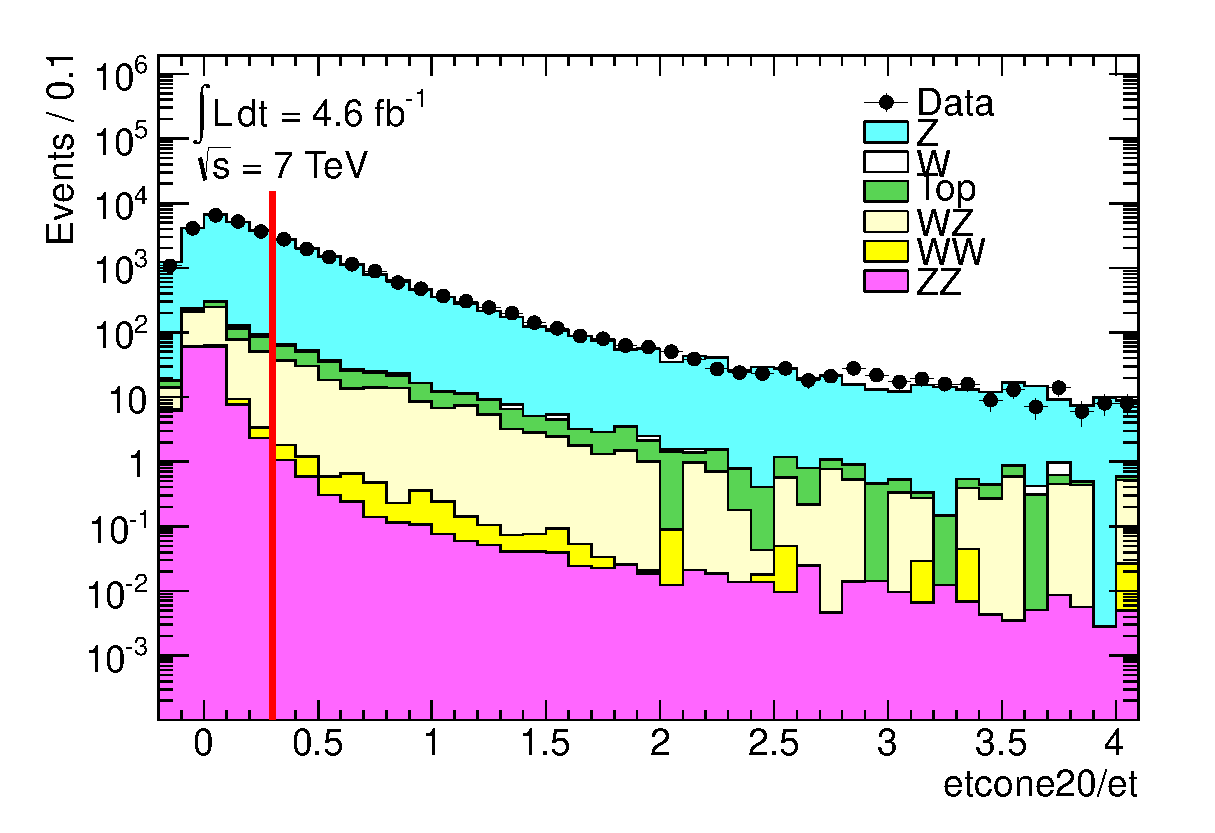
\includegraphics[width=0.47\textwidth]{ZplusX_log/CentralEl_etcone20rel}
        }
	\subfigure[]{
            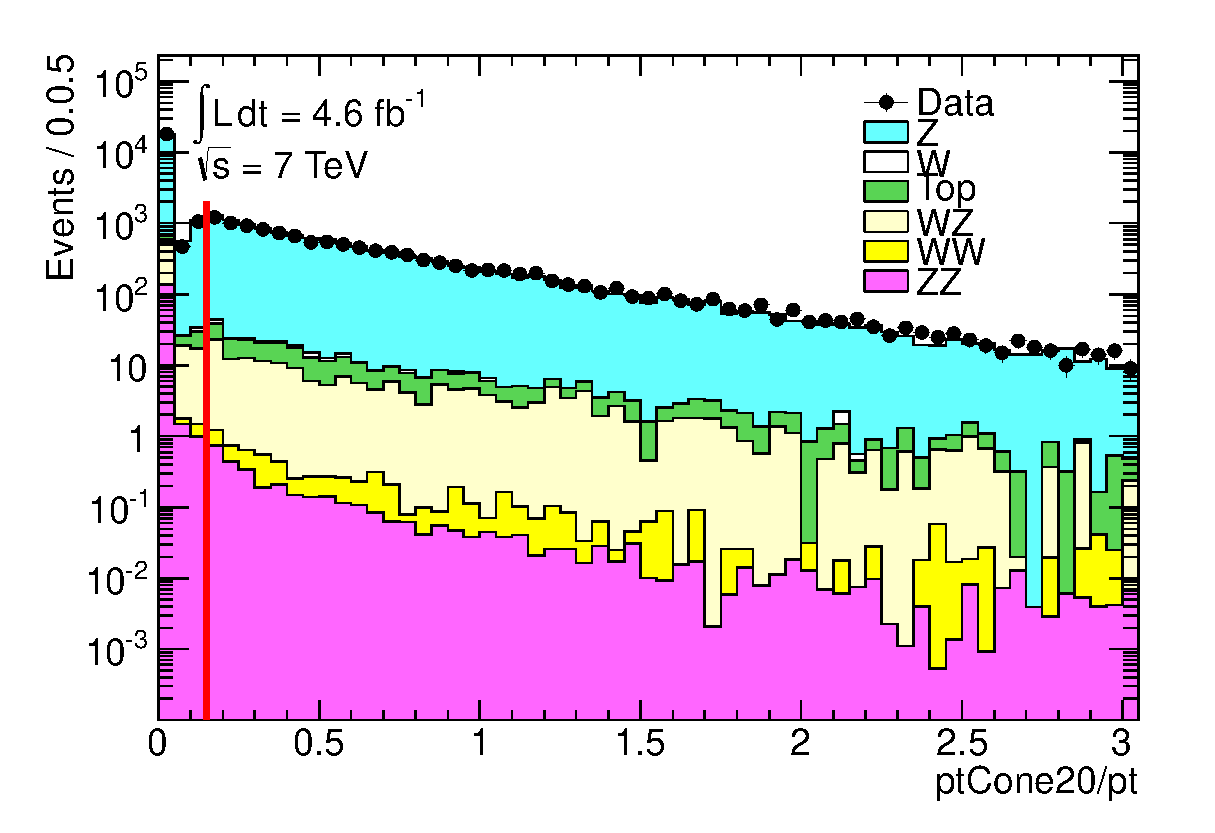
\includegraphics[width=0.47\textwidth]{ZplusX_log/CentralEl_ptcone20rel}
        }
	\subfigure[]{
            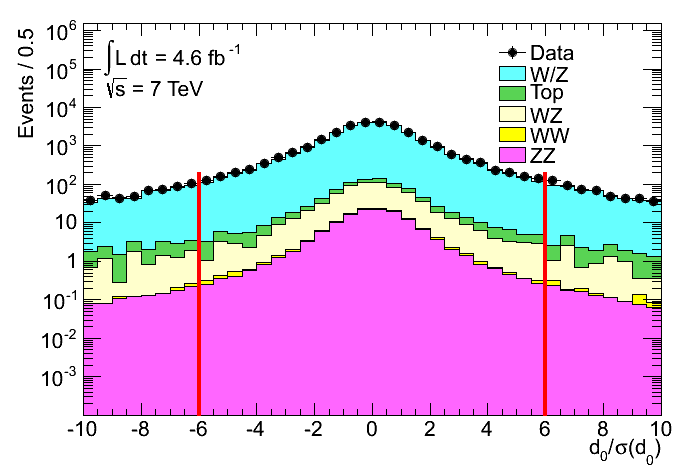
\includegraphics[width=0.47\textwidth]{ZplusX_log/CentralEl_d0Sig}
        }
	\subfigure[]{
            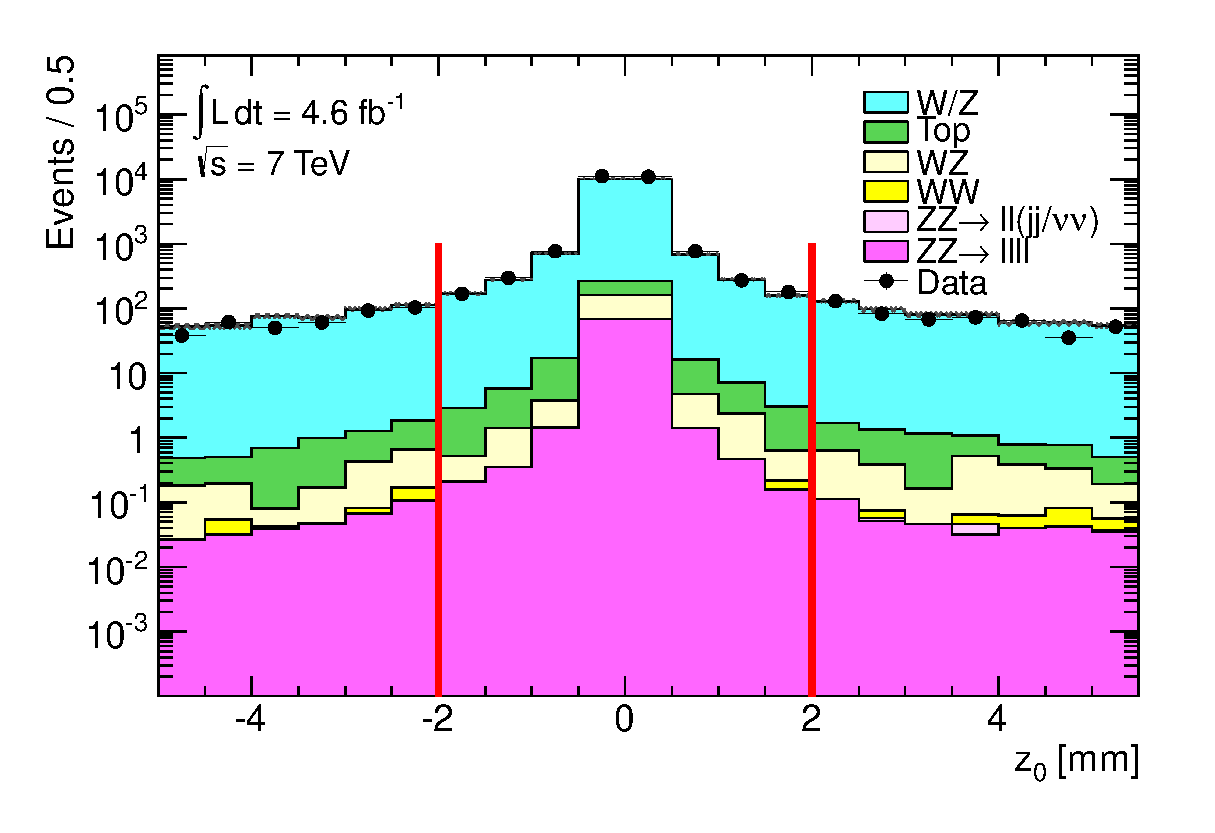
\includegraphics[width=0.47\textwidth]{ZplusX_log/CentralEl_z0}
        }
\caption[ Distributions of relative track and calorimeter isolation, \dzerosig\
and \zzero\ for additional electrons in events containing a dilepton pair with
mass \sstooos\ in 7~\tev\ data.]{Distributions of (a) relative calorimeter isolation, (b)
relative track isolation, (c) impact parameter significance \dzerosig,
and (d) longitudinal impact parameter \zzero\ for additional electrons in events
containing an \ossf\ \dilepton\ pair with
invariant mass \sstooos\ in 7~\tev\ data. The leptons forming the \dilepton\ pair are required to pass all of
the selection requirements described above, and one must match to the triggering
object and have \ptgt{25}. Additional electrons other than those forming the
\dilepton\ pair are required to pass
the kinematic selection requirements and the \loosePP\ identification
requirements; only these additional electrons are included in the plots.}
\label{fig:objsel-el}
\end{figure}

%\begin{figure}[h]
%\centering
%	\subfigure[]{
%            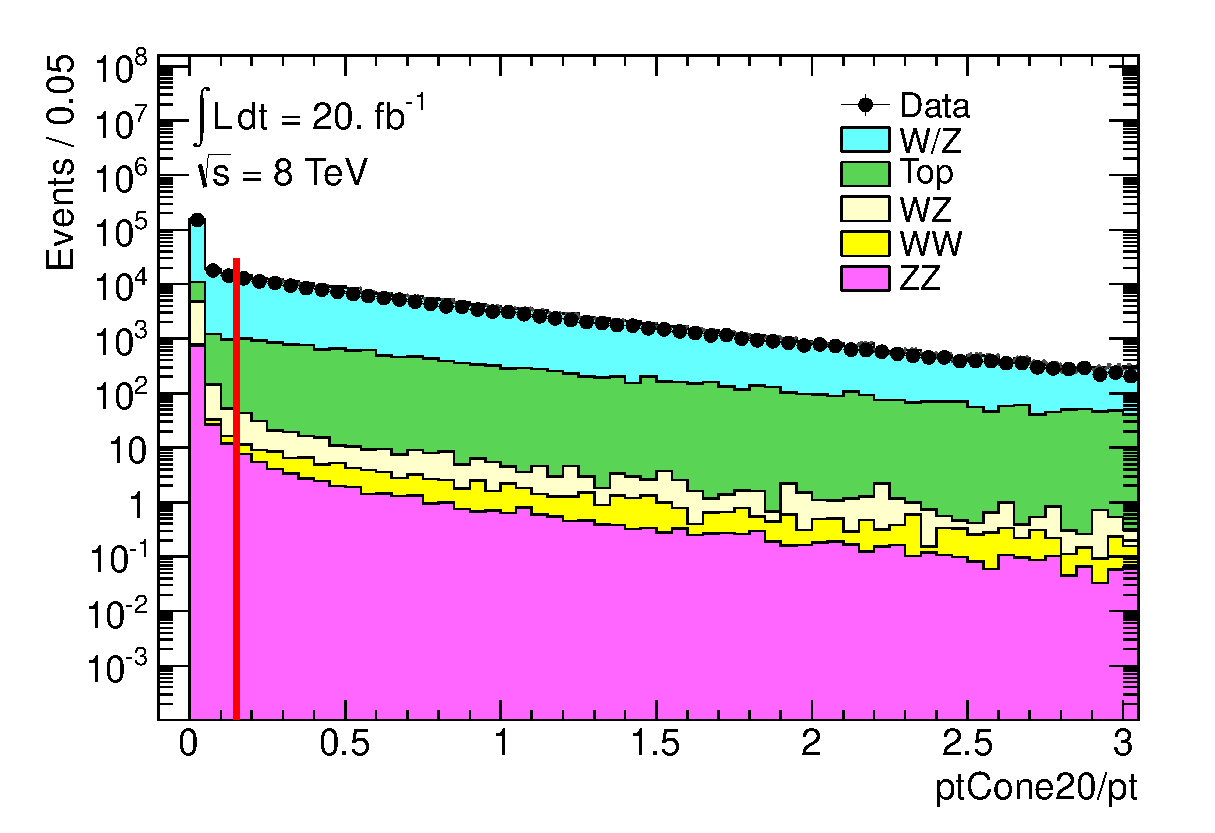
\includegraphics[width=0.47\textwidth]{ZplusX8TeV_log/CentralEl_ptcone20rel}
%        }
%	\subfigure[]{
%            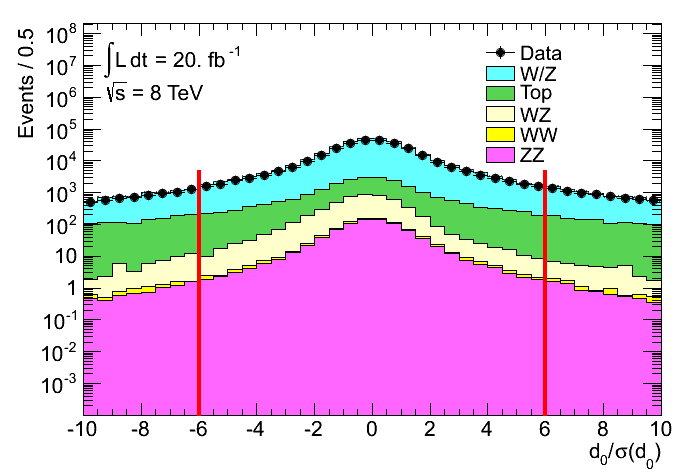
\includegraphics[width=0.47\textwidth]{ZplusX8TeV_log/CentralEl_d0Sig}
%        }
%	\subfigure[]{
%            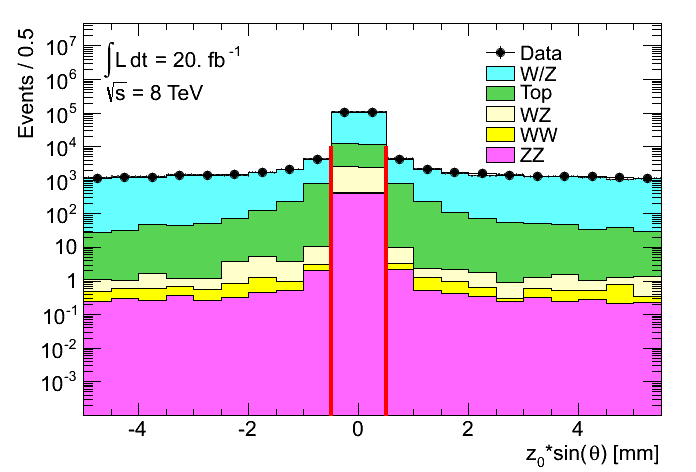
\includegraphics[width=0.47\textwidth]{ZplusX8TeV_log/CentralEl_z0sinTheta}
%        }
%\caption[ Distributions of relative track and calorimeter isolation, \dzerosig\
%and \zzero\ for additional electrons in events containing a dilepton pair with
%mass \sstooos\ in 7~\tev\ data.]{Distributions of (a) relative calorimeter isolation, (b)
%relative track isolation, (c) impact parameter significance \dzerosig,
%and (d) longitudinal impact parameter \zzero\ for additional electrons in events
%containing an \ossf\ \dilepton\ pair with
%invariant mass \sstooos\ in 7~\tev\ data. The leptons forming the \dilepton\ pair are required to pass all of
%the selection requirements described above, and one must match to the triggering
%object and have \ptgt{25}. Additional electrons other than those forming the
%\dilepton\ pair are required to pass
%the kinematic selection requirements and the \loosePP\ identification
%requirements; only these additional electrons are included in the plots.}
%\label{fig:objsel-el-eight}
%\end{figure}

%\begin{figure}[h]
%\centering
%	\subfigure[]{
%            \includegraphics[width=0.47\textwidth]{ObjSel/h_4l_ElEtCone20_log}
%        }
%	\subfigure[]{
%            \includegraphics[width=0.47\textwidth]{ObjSel/h_4l_ElPtCone20_log}
%        }
%	\subfigure[]{
%            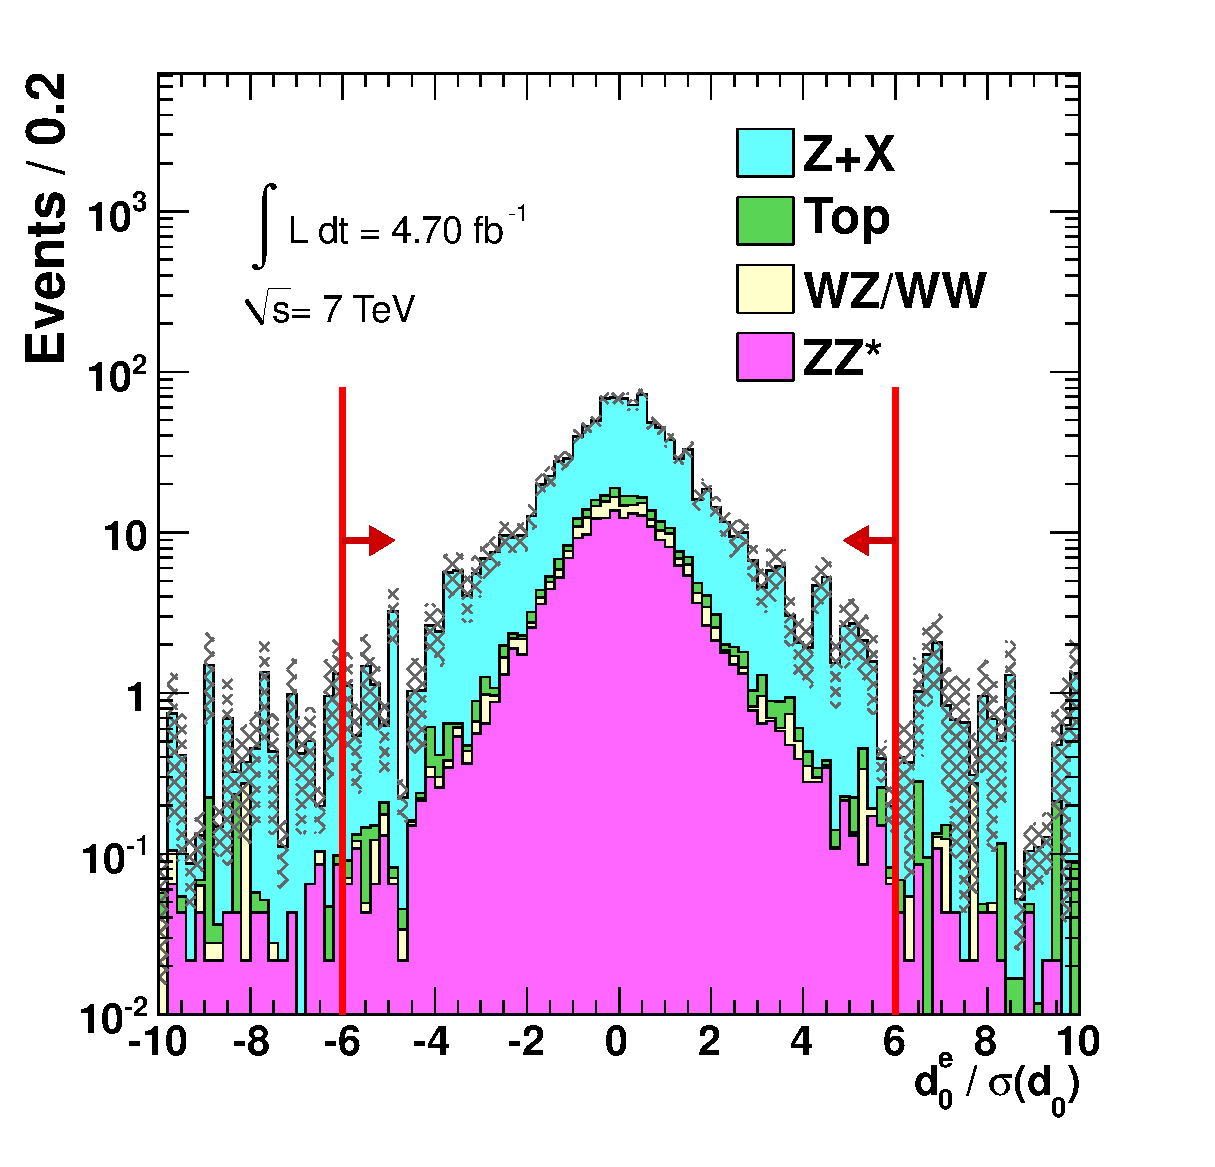
\includegraphics[width=0.47\textwidth]{ObjSel/h_4l_Electron_d0Sig_log}
%        }
%\caption[ ]{}
%\label{fig:objsel-el}
%\end{figure}
%
%\section{Muon Selection}
%\label{sec:objsel-mu}

\section{Muon Selection}
\label{sec:objsel-mu}

\begin{table}[]
  \centering
%   \vspace*{-1cm}
\small
  \begin{tabular}{ l  l l }
    \hline\hline 
      Requirement        & 7 \tev\ & 8 \tev\ \\ 
      \hline
      \bf{Central Muons} & \\
      Algorithm             & \staco                        & \same \\
      Type                  & \combined\ or Segment Tagged    & \same \\
      $\eta$                & $|\eta|<2.5$                  & \same \\
      $p_T$                 & $p_T > 7$ GeV                 & \same \\
      ID Track Quality      & & \\
       - B Layer Hits       & $\geq 1$                      & \same \\
       - Pixel Hits         & $\geq 2$                      &  $\geq 1$\\
       - SCT Hits           & $\geq 6$                      &  $\geq 5$\\
       - Silicon `Holes'    & $<3$                          & \same \\
       - TRT                & \multicolumn{1}{p{5cm}}{\raggedright
                                {\bf If \modetalt{1.9}:} 
                                Require $n_{hits}+n_{outliers}>5$ 
                                and $n_{outliers}/(n_{hits}+n_{outliers})<0.9$}
                                                            & \multicolumn{1}{p{5cm}}{\raggedright
                                                                {\bf If \modetabetween{0.1}{1.9}:} 
                                                                Require $n_{hits}+n_{outliers}>5$ 
                                                                and $n_{outliers}/(n_{hits}+n_{outliers})<0.9$} \\
                            & \multicolumn{1}{p{5cm}}{\raggedright
                                {\bf If \modetagt{1.9}:} 
                                If $n_{hits}+n_{outliers}>5$ 
                                require $n_{outliers}/(n_{hits}+n_{outliers})<0.9$} 
                                                            & \multicolumn{1}{p{5cm}}{\raggedright
                                                                {\bf If \modetagt{1.9} or \modetalt{0.1}:} 
                                                                If $n_{hits}+n_{outliers}>5$ 
                                                                require $n_{outliers}/(n_{hits}+n_{outliers})<0.9$} \\
      \zzero                & $|\zzero| < 2$ mm             & $|\zzero\sin(\theta)| < 0.5$ mm \\
      \dzerosig             & $|\dzerosig| < 3.5 $            & $|\dzerosig| < 3$ \\
      Track isolation       & \ptconetwentylt{0.15}         & \same   \\
      Calorimeter isolation & \etconetwentylt{0.3}          & \it{Not Applied} \\
      \hline
      \bf{Forward Muons} & \\
      Algorithm             & \staco                        & \same \\
      Type                  & \combined\ or Stand-Alone       & \same \\
      $\eta$                & \modetabetween{2.5}{2.7}      & \same \\
      $p_T$                 & $p_T > 10$ GeV                & \same \\
      Calorimeter isolation & \etconetwentylt{0.15}         & \same \\
      % This is a cut that is automatically satisfied by combined
      %MS Track Quality      & Hits in all 3 stations       & \same \\
       \multicolumn{3}{c}{\it \underline{Additional requirements for \combined\ Muons}} \\
      ID Track Quality      &                               &  \\
       - B Layer Hits       & $\geq 1$                      & \same \\
       - Pixel Hits         & $\geq 2$                      & $\geq 1$\\
       - SCT Hits           & $\geq 4$                      & $\geq 3$\\
       - Silicon `Holes'    & $<3$                          & \same \\
      \zzero                & $|\zzero| < 2$ mm             & $|\zzero\sin(\theta)| < 0.5$ mm \\
      \dzerosig             & $|\dzerosig| < 3.5 $          & $|\dzerosig| < 3$ \\
      \hline
      \multicolumn{2}{l}{\bf Calorimeter Tagged Muons} & \\
      Type                  & Calorimeter Tagged            & \same \\
      $\eta$                & \modetalt{0.1}                  & \same \\
      $p_T$                 & $p_T > 20$ GeV                & \same \\
      Quality               & Calorimeter Muon ID Cuts      & \same \\
      % This is a cut that is automatically satisfied by combined
      %MS Track Quality      & Hits in all 3 stations       & \same \\
      Overlap removal       & \multicolumn{1}{p{5cm}}{Remove 
                              if overlaps with a central 
                              muon in \deltaRlt{0.1}}  & \it{Same}\\
      \multicolumn{3}{c}{\it ID Track Quality, Track Isolation, Calorimeter
                                Isolation, \zzero, \dzerosig\ as central muons} \\
      %ID Track Quality      & As Central Muons              &  \\
      %Calorimeter isolation & \etconetwentylt{0.3}         & \same \\
      %Track isolation       & \ptconetwentylt{0.15}         & \same   \\
      %$z_0$                 & $|z_0| < 2$ mm                & $|z_0\sin(\theta)| < 0.5$ mm \\
      %$d_0$                 & $|d_0|/\sigma(d_0) < 3.5 $    & \same \\
                                                            
%
      %\bf{Central Electron Selection} & \\
      %Algorthim             & Standard (with GSF refit)     & Standard \\
      %Quality               & \multicolumn{2}{c}{\texttt{(OQ  AND 1446 == 0})} \\
      %ID cut                & \multicolumn{2}{c}{\loosePP}       \\
      %$\eta$                & \multicolumn{2}{c}{$|\eta|<2.47$} \\
      %$E_T$                 & \multicolumn{2}{c}{$E_T > 7$ GeV} \\
      %$z_0$                 & \multicolumn{2}{c}{$z_0 < 2$ mm} \\
      %$d_0$                 & \multicolumn{2}{c}{$|d_0|/\sigma(d_0) < 6 $} \\
      %Track isolation       & \multicolumn{2}{c}{\ptconetwentylt{0.15}}   \\
      %Calorimeter isolation & \etconetwentylt{0.3}          & \it{Not Applied} \\
      %Overlap removal       & \multicolumn{2}{c}{a) Remove $e$ if $\Delta R < 0.1$ from $\mu$} \\
      %                      & \multicolumn{2}{c}{b) Remove lowest $E_T$ $e$ in \deltaRlt{0.1} from another $e$} \\ 
      %\hline
      %\bf{Forward Electron Selection:} & \\
      %Alogirthm             & \multicolumn{2}{c}{Forward} \\
      %Quality               & \multicolumn{2}{c}{\texttt{(OQ  AND 1446 == 0)}}  \\
      %ID cut                & \multicolumn{2}{c}{Tight} \\
      %$\eta$                & \multicolumn{2}{c}{$2.50<|\eta|<3.16$} \\
      %$E_T$                 & \multicolumn{2}{c}{$E_T > 20$ GeV} \\
      %Overlap removal       & \multicolumn{2}{p{8cm}}{\centering Remove if overlaps with central electron or any muon in \deltaRlt{0.1}} \\
    \hline \hline
  \end{tabular}
   \caption{Muon selection requirements.}
   \label{table:objsel-mu}
\end{table}

Muon reconstruction was described in~\sec{reco-mu}. Three distinct categories of
muons are used in this analysis: `central' muons with \modetalt{2.5} and
`forward' muons with \modetabetween{2.5}{2.7}, both reconstructed with the
\staco\ algorithm, and calorimeter tagged muons with \modetalt{0.1},
reconstructed without using the muon spectrometer. As for electrons, additional
selection requirements are applied to select muons likely to have originated from
\Z\ boson decays and to reject backgrounds. The muon selection requirements are
summarised in~\tab{objsel-mu} are described in more detail below. 

\subsection{Central Muon Selection}

Central muons may be either \combined\ (with a full MS and ID track) or
\segmentTagged\ (with a full ID track but only an MS track segment), and have $\pt>7$ GeV
and \modetalt{2.47}.

As for electrons, track and calorimeter isolation requirements are imposed to
reject backgrounds. In the case of muons this is mainly from heavy flavour
decays in jets and `punch-through' of hadrons into the muon spectrometer.  The
track isolation is defined in the same way as for electrons, and as for
electrons the requirement
is \ptconetwentylt{0.15}.  The calorimeter isolation variable is defined in a
similar way as for electrons, however the size of the `core' deposit of energy
attributed to the muon is smaller than in the case of electron isolation, and
varies by calorimeter component depending on the expected muon energy deposition
pattern (e.g. a single cell in the EM pre-sampler, but a 3x3 grid of cells in the second
layer of the EM calorimeter). The calorimeter isolation requirement is
\etconetwentylt{0.3}, and as for electrons is only applied to the 7~\tev\ data.

To ensure that the candidates come from the primary vertex, the magnitude of the
longitudinal impact parameter with respect to the primary vertex, $|z_0|$ must
be less than 2 mm for the 7~\tev\ data. For the 8~\tev\ data, the requirement is
$|z_0\sin(\theta)|<0.5$ mm. The magnitude of the transverse impact parameter
significance, $|\dzerosig|$ is required to be less than 3.5(3) in the 7(8)~\tev\
analysis. The selection for muons is tighter than for electrons, since because
muons do not emit \brem\ to the same extent as electrons, the track fit and thus
the resolution of the impact parameter is improved, so tighter requirements can
be made whilst maintaining high signal efficiency.

The inner detector tracks associated with central muons must have a minimum
number of hits in each silicon sub-detector to ensure good track quality. For
7~\tev\ data the requirements are: at least 1 hit in the b-layer, $2$ hits in all Pixel
layers, $6$ hits in the SCT, and less than 3 holes (no hit in a layer crossed by the
track) in all silicon layers. For all silicon hit conditions, dead sensors count
as hits observed, not as holes.  Finally, a pseudo-rapidity dependent condition
on TRT hits and outliers is applied to ensure that the TRT extension of the
track is successful within the $\eta$ acceptance of the TRT (TRT hits can be
associated as outliers when the extension is not successful): for $|\eta| <
1.9$, require $\mathrm{hits}+\mathrm{outliers} > 6$ and $\mathrm{outliers} < 0.9
\times (\mathrm{outliers}+\mathrm{hits})$; for $|\eta| > 1.9$, if
$\mathrm{hits}+\mathrm{outliers} > 6$, require $\mathrm{outliers} < 0.9 \times
(\mathrm{outliers}+\mathrm{hits})$. For 8~\tev\ data, the
requirements are slightly loosened in order to recover efficiency losses arising
from higher pileup in 2012; this was not found to increase the misidentification rate significantly;
see~\tab{objsel-mu} for details of the changes.


\begin{table}
\begin{tabular}{l|c|c|c|c}
\hline\hline
Cut & 7 TeV &  & 8 TeV &  \\
\hline
                          All &  $100.0 \pm 0.0$\% &          $ \pm $\% &  $100.0 \pm 0.0$\% &         $ \pm $\% \\
                $p_{T}>7$ GeV &   $99.9 \pm 0.0$\% &   $99.9 \pm 0.0$\% &   $99.9 \pm 0.0$\% &  $99.9 \pm 0.0$\% \\
                   Track Hits &   $98.6 \pm 0.0$\% &   $98.8 \pm 0.0$\% &   $99.2 \pm 0.0$\% &  $99.2 \pm 0.0$\% \\
                $|z0| < 2$ mm &   $98.6 \pm 0.0$\% &  $100.0 \pm 0.0$\% &   $99.1 \pm 0.0$\% &  $99.9 \pm 0.0$\% \\
$|d_{0}/\sigma(d_{0})| < 3.5$ &   $98.3 \pm 0.0$\% &   $99.7 \pm 0.0$\% &   $98.5 \pm 0.0$\% &  $99.4 \pm 0.0$\% \\
              Track Isolation &   $97.6 \pm 0.1$\% &   $99.3 \pm 0.0$\% &   $97.3 \pm 0.0$\% &  $98.8 \pm 0.0$\% \\
         Calorimter Isolation &   $97.0 \pm 0.1$\% &   $99.5 \pm 0.0$\% &    $0.0 \pm 0.0$\% &         $ \pm $\% \\
\hline\hline
\end{tabular}
\caption{Central Muons}
\end{table}

\subsection{Forward Muon Selection}

Muons in the region \modetabetween{2.5}{2.7} are required to have a full muon
spectrometer track with hits in each station of the spectrometer and must have
\ptgt{10}. Although the
inner detector only extends to \modetaeq{2.5}, the complicated nature of the
magnetic field makes it possible for some muons up to \modetalt{2.6} to be
combined with an ID track, forming \combined\ muons; those that do not have an
ID track are termed Stand Alone.~\fig{fwdmu-frac-combined} shows the fraction
of forward muons which are \combined\ as a function of $\eta$. In data reconstructed in 2012 muons without a
full ID track may be combined with pixel detector `tracklets' up to
\modetalt{2.65}. Such `Silicon Associated' muons benefit from improved vertex
parameter estimation, but are otherwise treated as Stand Alone. 

\begin{figure}[h]
\centering
	\subfigure{
            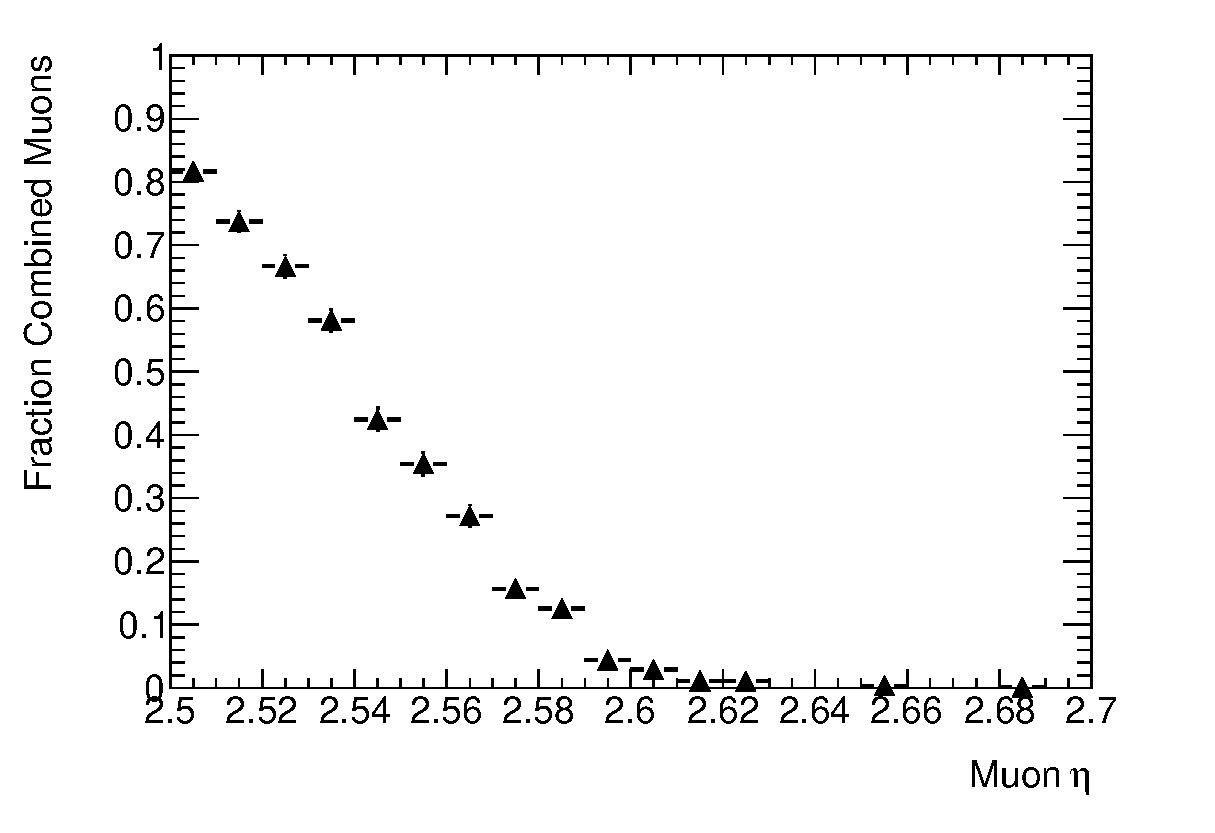
\includegraphics[width=0.65\textwidth]{ObjSel/fwdmu_frac_combined_mc11}
        }
\caption[Fraction of forward muons which are \combined\ muons as a function of
$\eta$]{Fraction of forward
muons which are have an ID track and are \combined\ muons, as a function of
$\eta$. The fractions are estimated from \mc\ simulation; the error bars show
statistical uncertainties.}
\label{fig:fwdmu-frac-combined}
\end{figure}

Since not all forward muons
have tracks, a track isolation requirement is not applied; instead a tighter calorimeter isolation
requirement is applied to forward muons: \etconetwentylt{0.15}. This is applied
to both the 7~\tev\ and the 8~\tev\ data.

For forward muons with an ID track, a set of quality
cuts are applied to the number of hits in the silicon detectors, similar to the
cuts for central muons but slightly looser. For 7~\tev\ data,
the requirements are: at least 1 hit in the b-layer, $2$ in all Pixel layers,
$4$ in the SCT, and less than 3 holes 
in all silicon layers. No cut is applied to the number of TRT hits, as forward
muon tracks are generall outside of the acceptance of the TRT. As for
central muons, the requirements were relaxed slightly for 2012 data.
Forward muons with an ID track are required to satisfy the same
\zzero\ and \dzerosig\ requirements as central muons.

\begin{table}[htbp]
\centering
\begin{tabular}{l|c|c|c|c}
\hline\hline
Cut & 7 TeV &  & 8 TeV &  \\
\hline
                          All &  $100.0 \pm 0.0$\% &          $ \pm $\% &  $100.0 \pm 0.0$\% &         $ \pm $\% \\
                $p_{T}>7$ GeV &   $93.1 \pm 0.6$\% &   $93.1 \pm 0.6$\% &   $94.5 \pm 0.5$\% &  $94.5 \pm 0.5$\% \\
                      Quality &   $92.7 \pm 0.7$\% &   $99.6 \pm 0.2$\% &   $94.0 \pm 0.5$\% &  $99.4 \pm 0.2$\% \\
                   Track Hits &   $87.6 \pm 0.9$\% &   $94.5 \pm 0.6$\% &   $89.6 \pm 0.6$\% &  $95.4 \pm 0.4$\% \\
                $|z0| < 2$ mm &   $87.6 \pm 0.9$\% &  $100.0 \pm 0.0$\% &   $89.1 \pm 0.6$\% &  $99.4 \pm 0.1$\% \\
$|d_{0}/\sigma(d_{0})| < 3.5$ &   $86.8 \pm 0.9$\% &   $99.1 \pm 0.3$\% &   $88.2 \pm 0.6$\% &  $98.9 \pm 0.2$\% \\
              Track Isolation &   $86.1 \pm 0.9$\% &   $99.2 \pm 0.2$\% &   $87.1 \pm 0.7$\% &  $98.8 \pm 0.2$\% \\
         Calorimter Isolation &   $85.6 \pm 0.9$\% &   $99.5 \pm 0.2$\% &    $0.0 \pm 0.0$\% &         $ \pm $\% \\
\hline\hline
\end{tabular}
\caption{Forward Muons}
\end{table}

\subsection{Calorimeter Tagged Muon Selection}

Calorimeter tagged muons are used to recover efficiency at \modetalt{0.1} where
there is a gap in the muon-spectrometer. Due to the higher level of fakes from jets and
electrons at low \pt, and the difficulty of measuring the identification
efficiency at low \pt, the \pt\ requirement for calorimeter tagged muons is
\ptgt{20}. They are required to pass either the cut or
the likelihood based calorimeter tagged muon identification requirements described
in~\sec{reco-mu-reco}, and are not selected if they overlap with a selected
central muon within \deltaRlt{0.1}. Calorimeter tagged muons must satisfy the
same track and calorimeter isolation, ID track quality, \zzero\ and \dzerosig\
requirements as central muons.

\begin{table}[htbp]
\centering
\begin{tabular}{l|c|c|c|c}
\hline\hline
Cut & 7 TeV &  & 8 TeV &  \\
\hline
                          All &  $100.0 \pm 0.0$\% &         $ \pm $\% &  $100.0 \pm 0.0$\% &         $ \pm $\% \\
               $p_{T}>10$ GeV &   $97.1 \pm 0.7$\% &  $97.1 \pm 0.7$\% &   $97.6 \pm 0.5$\% &  $97.6 \pm 0.5$\% \\
                   Track Hits &   $91.8 \pm 1.1$\% &  $94.6 \pm 1.0$\% &   $94.1 \pm 0.8$\% &  $96.4 \pm 0.6$\% \\
                $|z0| < 2$ mm &   $91.8 \pm 1.1$\% &  $99.9 \pm 0.1$\% &   $93.8 \pm 0.8$\% &  $99.7 \pm 0.2$\% \\
$|d_{0}/\sigma(d_{0})| < 3.5$ &   $91.4 \pm 1.1$\% &  $99.6 \pm 0.2$\% &   $92.8 \pm 0.9$\% &  $98.9 \pm 0.5$\% \\
         Calorimter Isolation &   $90.0 \pm 1.2$\% &  $98.5 \pm 0.5$\% &   $90.9 \pm 1.0$\% &  $98.0 \pm 0.5$\% \\
\hline\hline
\end{tabular}
\caption{Forward Muons}
\end{table}

%\begin{figure}[h]
%\centering
%	\subfigure[]{
%            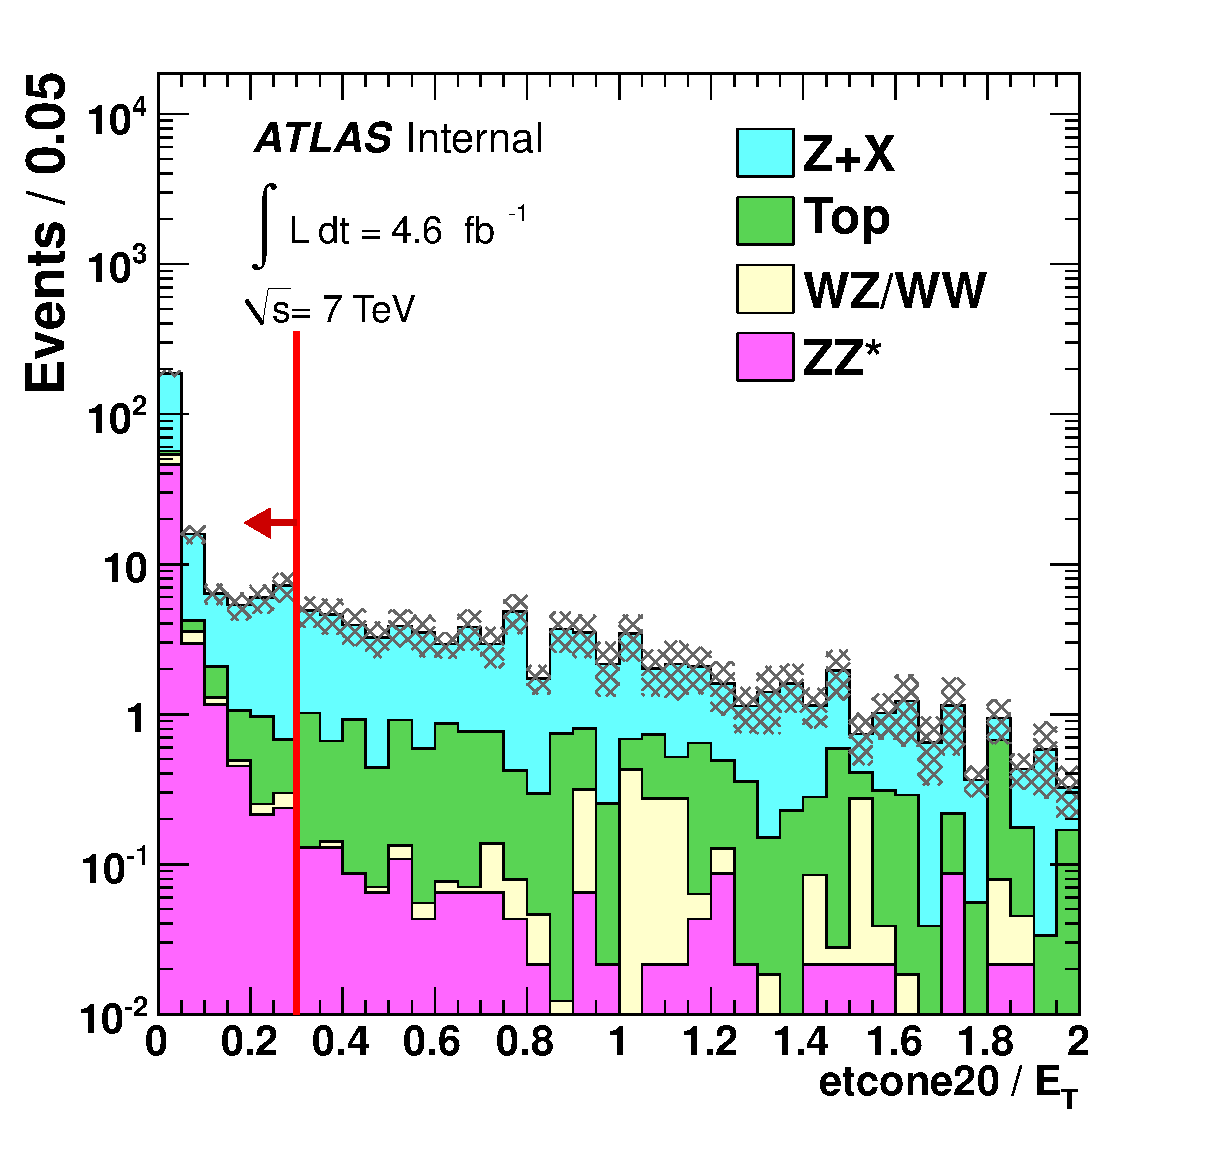
\includegraphics[width=0.47\textwidth]{ObjSel/h_4l_MuEtCone20_log}
%        }
%	\subfigure[]{
%            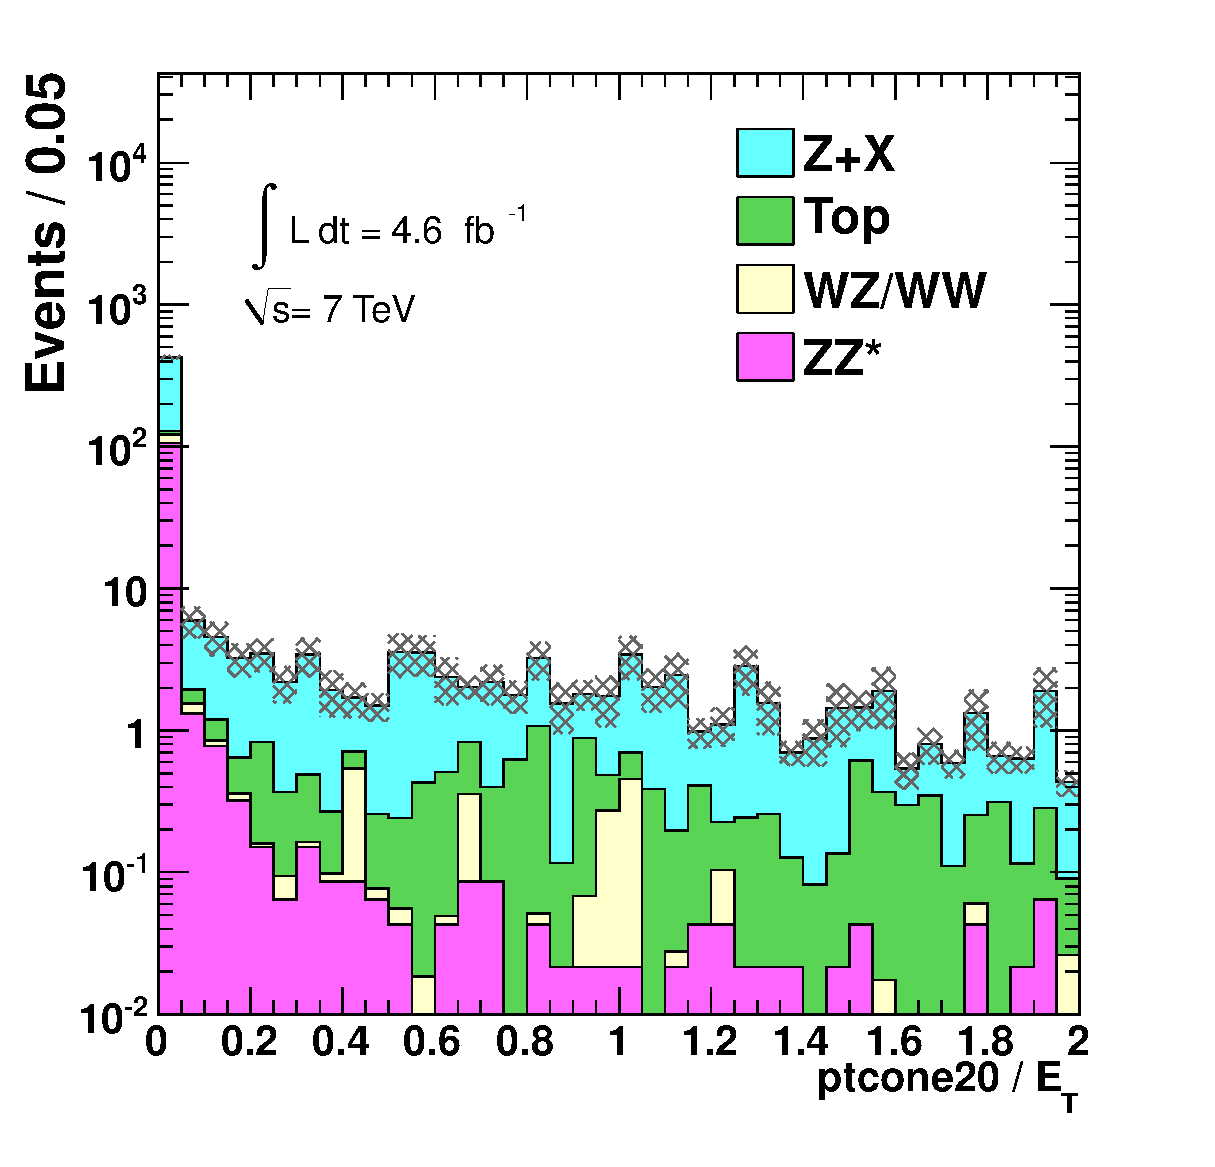
\includegraphics[width=0.47\textwidth]{ObjSel/h_4l_MuPtCone20_log}
%        }
%	\subfigure[]{
%            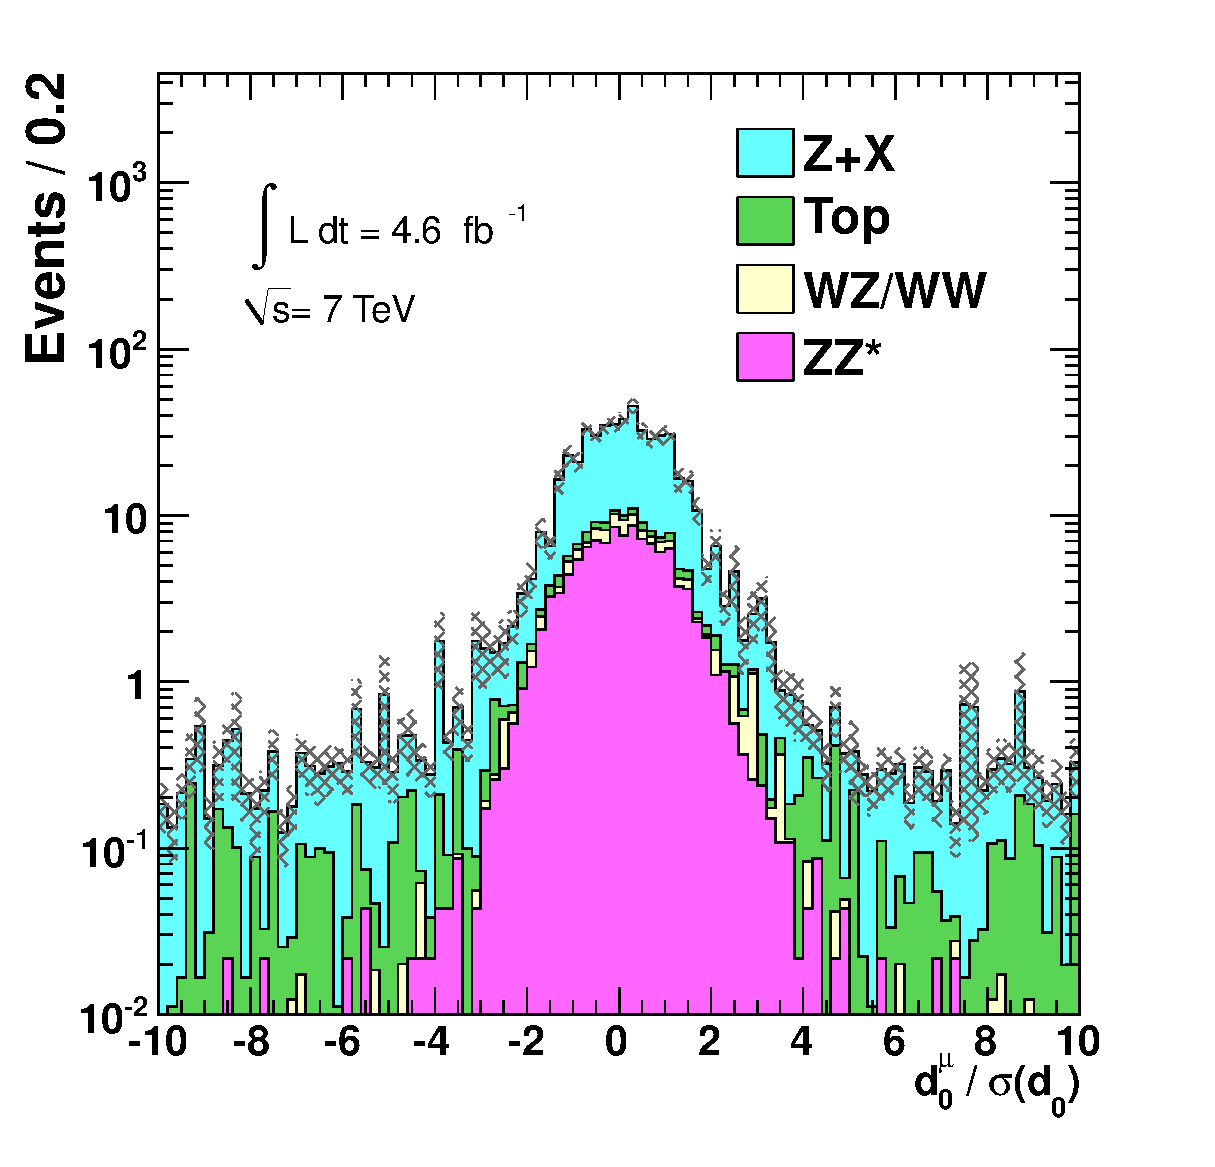
\includegraphics[width=0.47\textwidth]{ObjSel/h_4l_Muon_d0Sig_log}
%        }
%\caption[ ]{}
%\label{fig:objsel-mu}
%\end{figure}

\subsection{Muon distributions}

To motivate the muon isolation, \dzerosig\ and \zzero\ requirements described
above, \fig{objsel-mu} shows the distribution of these variables in 7~\tev\ data for additional
muons in events with an \ossf\ \dilepton\ pair with invariant mass \sstooos.
Similarly to the electron distributions, the leptons forming the \dilepton\ pair are required to pass all of
the selection requirements described above, and one must match to the triggering
object and have \ptgt{25}. Any additional muons in the event are required to pass
the kinematic (\pt,$\eta$) selection requirements, and the distributions of the isolation, \dzerosig\ and \zzero\
variables for these additional muons are shown in the plots. 

As for electrons, in the \WZ\ and \ZZ\ processes the additional muons 
are mainly prompt isolated leptons from \W\ or \Z\ decays. In the \Zll,
\ttbar\ and \WW\ processes, the additional muons mainly arise from muons from
hadronic decays in jets or `punch-through' of hadrons to the muon spectrometer.
These `background' muons tend to be less isolated, and have broader \dzerosig\
and \zzero\ distributions. Whilst the \mc\ models the shape of the distribution
fairly well, the number of additional muons observed in date is much higher than
predicted by the simulation.

\begin{figure}[h]
\centering
	\subfigure[]{
            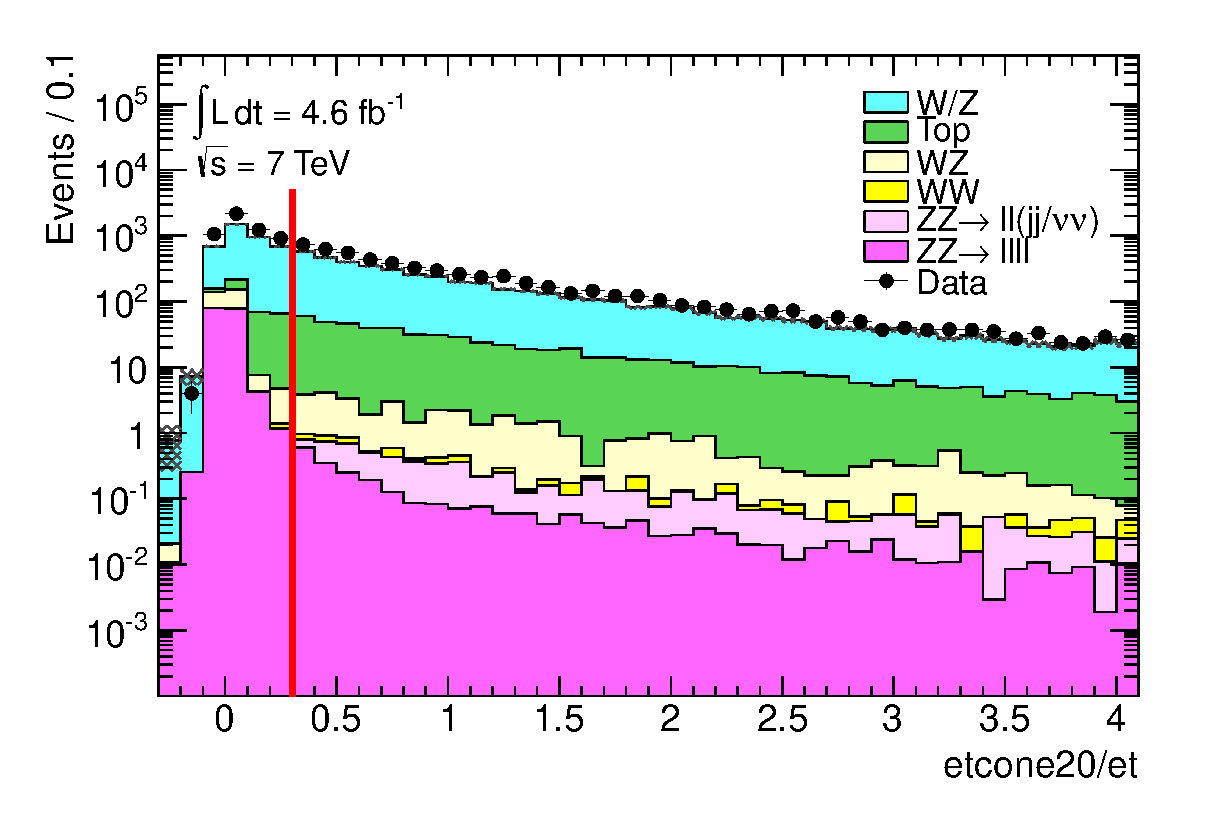
\includegraphics[width=0.47\textwidth]{ZplusX_log/CentralMu_etcone20rel}
        }
	\subfigure[]{
            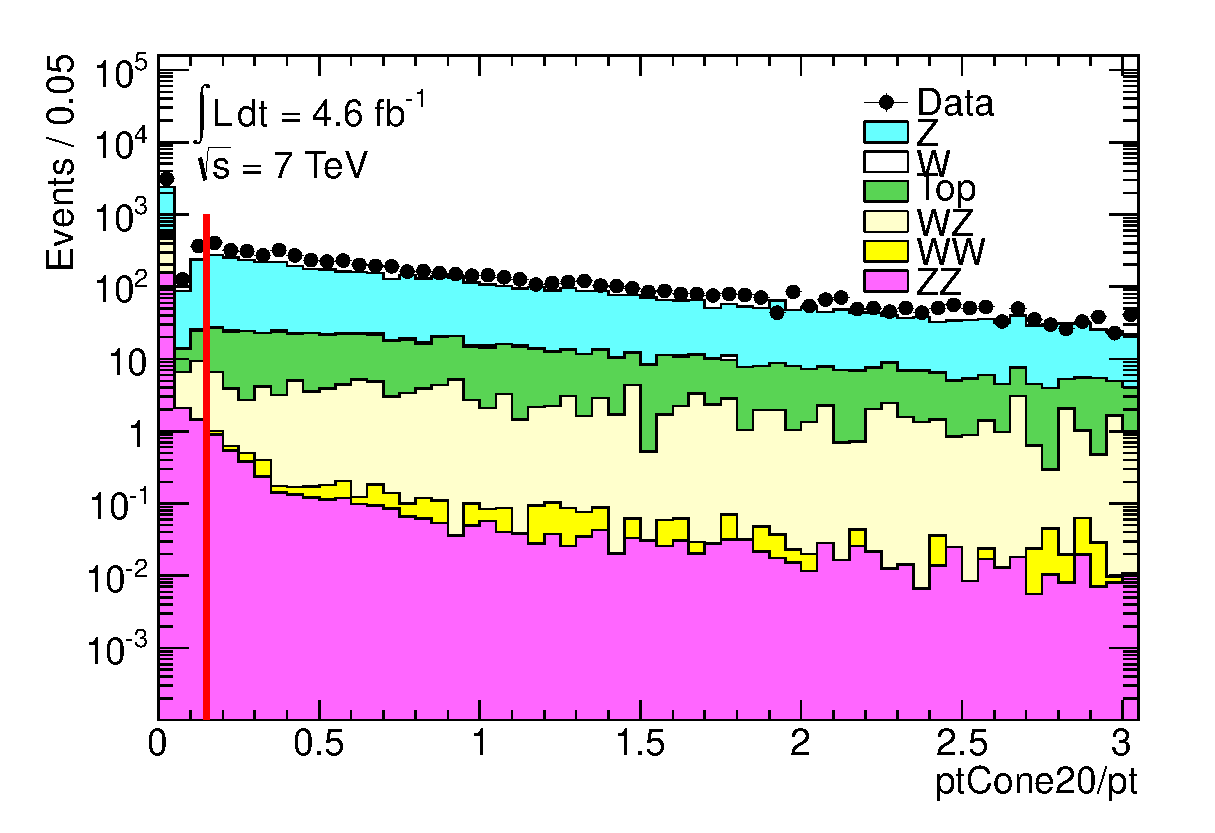
\includegraphics[width=0.47\textwidth]{ZplusX_log/CentralMu_ptcone20rel}
        }
	\subfigure[]{
            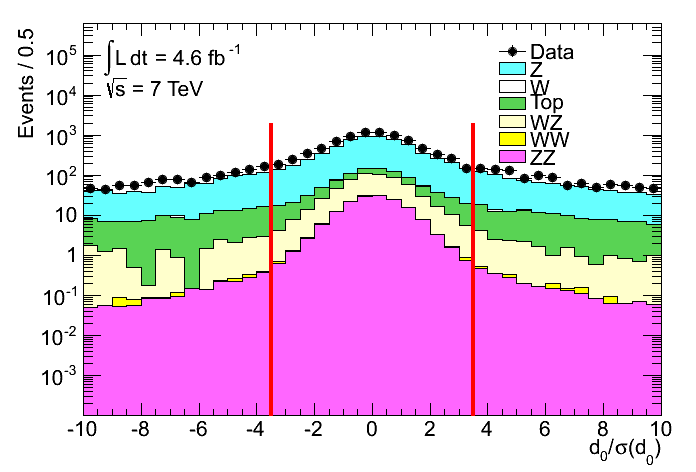
\includegraphics[width=0.47\textwidth]{ZplusX_log/CentralMu_d0Sig}
        }
	\subfigure[]{
            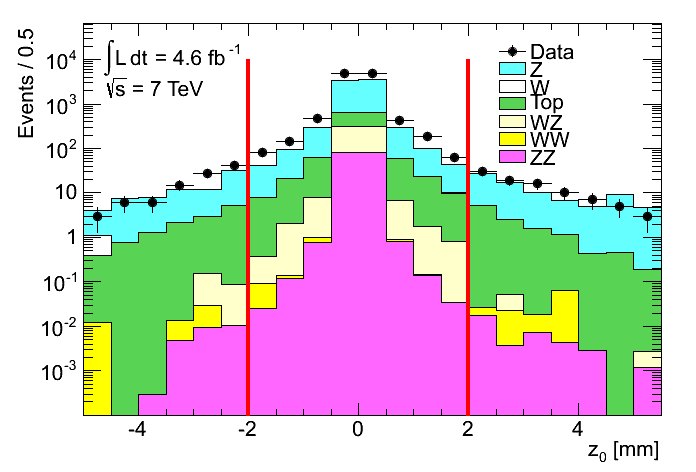
\includegraphics[width=0.47\textwidth]{ZplusX_log/CentralMu_z0}
        }
    \caption[ Distributions of relative track and calorimeter isolation, \dzerosig\
    and \zzero\ for additional muons in events containing a dilepton pair with mass
    \sstooos\ in 7~\tev\ data.]
    {Distributions of (a) relative calorimeter isolation,
    (b) relative track isolation, (c) impact parameter significance \dzerosig\ and
    (d) longitudinal impact parameter \zzero\ for additional muons
    in events containing an \ossf\ \dilepton\ pair with invariant mass \sstooos\
    in the 7~\tev\ data.
    The leptons forming the \dilepton\ pair are required to pass all of the
    selection requirements described above, and one must match to the triggering
    object with \ptgt{25}. Any additional muons, other than those forming the
    \dilepton\ pair, are required to pass the kinematic selection requirements; only
    these additional muons are included in the plots.}
\label{fig:objsel-mu}
\end{figure}
%\section{Jet Selection}

\section{Triggers}
\label{sec:triggers}

Candidate \ZZ\ events in are triggered on using the lowest threshold un-prescaled single-electron or
single-muon triggers, as descried in Section~\ref{sec:reco-el-triggers}
and~\ref{sec:reco-mu-triggers}. For the \eemm\ final state, the event may be selected using either
the electron or the muon trigger. The triggers used in the
different data taking periods and the
associated integrated luminosities are shown in~\tab{objSel-trigger-el} for the electron
triggers and~\tab{objSel-trigger-mu} for the muon triggers.

\begin{table}[htbp]
\begin{center}
%\small
\begin{tabular}{lccc p{5cm}}
\hline \hline
Period & Trigger & \pt\ Threshold (GeV) & Int. Luminosity (\ifb) \\
\hline
\multicolumn{3}{l}{ \bf 2011 (7~\tev\ data) } \\
B - I & \texttt{e20\_medium} & 20 &  1.65 \\
J - K & \texttt{e22\_medium} & 22 & 0.91 \\
L - M & \texttt{e22vh\_medium1} & 22 & 2.76 \\ \hline
%L - M & \texttt{e22vh\_medium1} & 22 & 2.76 & Variable L1 thresholds; hadronic leakage requirement \\ \hline
\hline
\multicolumn{3}{l}{ \bf 2012 (8~\tev\ data) } \\
A - M & \multicolumn{1}{p{4cm}}{\centering \texttt{e24vhi\_medium1} $||$ \texttt{e60\_medium1}} & 24 & \LumiTotalReadyTwentyTwelve \\
\hline\hline
\end{tabular}
\end{center}
\caption{Electron triggers used in the different data taking periods.}
\label{table:objSel-trigger-el}
\end{table}

\begin{table}[htbp]
\begin{center}
%\small
\begin{tabular}{lccc p{5cm}}
\hline \hline
Period & Trigger & \pt\ Threshold (GeV) & Int. Luminosity (\ifb) \\
\hline
\multicolumn{3}{l}{ \bf 2011 (7~\tev\ data) } \\
B - I & \texttt{mu18\_MG} & 18 &  1.65 \\
J - M & \texttt{mu18\_MG\_medium} & 18 & 3.67 \\
%L - M & \texttt{e22vh\_medium1} & 22 & 2.76 & Variable L1 thresholds; hadronic leakage requirement \\ \hline
\hline
\multicolumn{3}{l}{ \bf 2012 (8~\tev\ data) } \\
A - M & \multicolumn{1}{p{4cm}}{\centering \texttt{mu24i\_tight} $||$ \texttt{mu36\_tight}} & 24 & \LumiTotalReadyTwentyTwelve \\
\hline\hline
\end{tabular}
\end{center}
\caption{Muon triggers used in the different data taking periods.}
\label{table:objSel-trigger-mu}
\end{table}

At least one of the selected leptons in triggered events must match to the
object that caused the trigger to fire. Such leptons are referred to as 
\intro{trigger-matched} leptons. To reduce uncertainties associated with the
trigger efficiency measurement, to be considered trigger matched,
a lepton must have a \pt\ such that it is on the efficiency plateau of the
trigger, and must also satisfy the same identification requirements as
used in the trigger. Trigger-matched electrons in both the 7~\tev\ and the
8~\tev data
are required to have \ptgt{25}, cluster \modetalt{2.47} and to pass the \mediumPP\
requirements. Trigger matched muons are required to be \combined\ muons, have
\modetalt{2.4} and have $\pt > 20 (25)$ \gev\ in the 7(8)~\tev\ data.

\subsection{Trigger Efficiencies}

The efficiency for a single lepton to fire the trigger is measured in data using
\Zll\ events. Events are triggered on by a `tag' lepton; the efficiency for
the second `probe' lepton to fire the trigger is then measured. By comparing the
efficiencies in data and in \mc\ simulation, scale-factors are derived to
correct the single lepton trigger efficiencies in the simulation to those
observed in data.  This is translated to an event-level trigger efficiency
scale-factor using the following formula:

\begin{equation}
\label{eqn:triggerEffSF}
  SF =  { \frac{ {1 - \prod_{n=1}^{N_l} (1 - \epsilon_{Data,l_n})}} {1 - \prod_{n=1}^{N_l} (1 - \epsilon_{MC,l_n})} }
\end{equation}
where $N_l$ is the number of leptons passing the trigger-matching kinematic and
identification requirements
given above (not necessarily equal to the number of trigger-matched leptons),
$\epsilon_{Data,l_n}$ is the observed single-lepton trigger efficiency in data
for a lepton of flavour flavor $l_n$, and $\epsilon_{MC,l_n}$ is
the corresponding efficiency simulated in the MC. 
%The systematic uncertainty associated with the scale factors for
%muon triggers is $0.2\%$ and for electron triggers is $\sim1\%$. 

Event-level trigger efficiencies for \ZZ\ events passing the full event
selection described in the next section are listed in~\tab{triggerMCeff}. They
are derived from simulation after applying the trigger efficiency scale-factors
described above.

\begin{table}[htbp]
\begin{center}
\small
\renewcommand\arraystretch{1.05}
\begin{tabular}{llll}
\hline \hline
Channel & \multicolumn{3}{c}{Trigger Efficiency [\%]} \\
\hline
      & \ZZ\ Selection (7~\tev)     & \ZZs\ Selection  (7~\tev)             & \ZZ\ Selection (8~\tev)   \\
        \hline
        \eeee\  & 99.69 \errSym{0.08} \errSym{0.02}  & 99.38 \errSym{0.10} \errSym{0.03} & 99.89 \errSym{0.02} \errSym{0.03}\\
        \mmmm\  & 98.50 \errSym{0.15} \errSym{0.14}  & 97.68 \errSym{0.17} \errSym{0.18} & 98.10 \errSym{0.10} \errSym{0.20}\\
        \eemm   & 99.52 \errSym{0.07} \errSym{0.06}  & 99.06 \errSym{0.08} \errSym{0.08} & 99.49 \errSym{0.05} \errSym{0.09}\\
        \llll   & 99.23 \errSym{0.06} \errSym{0.08}  & 98.67 \errSym{0.07} \errSym{0.10} & 99.14 \errSym{0.04} \errSym{0.11}\\
% From Note
% systematics seem a bit smaller than before - updated tool maybe?
%                   $eeee$ & 100.0$^{+0.0}_{-0.4}$   & 99.6$^{+0.2}_{-0.5}$ & 99.89\errSym{0.02}\errSym{0.03}\\
%           $\mu\mu\mu\mu$ & 98.7$^{+0.4}_{-0.6}$    & 98.2$^{+0.4}_{-0.5}$ & 98.10\errSym{0.01}\errSym{0.20}\\
%               $ee\mu\mu$ & 99.6$^{+0.2}_{-0.3}$    & 98.8$^{+0.3}_{-0.4}$ & 99.49\errSym{0.05}\errSym{0.09}\\
%                   $llll$ & 99.4$^{+0.2}_{-0.2}$    & 98.8$^{+0.2}_{-0.2}$ & 99.14\errSym{0.04}\errSym{0.11}\\
    \hline \hline
\end{tabular}
\defaultArrayStretch
\end{center}
\caption[Trigger efficiencies for \ZZ\ events passing the full event selection 
excluding the trigger requirement and the requirement for a reconstructed lepton to match to
the triggering object.]
{Trigger efficiencies for \ZZ\ events passing the full event selection 
excluding the trigger requirement and the requirement for a reconstructed lepton to match to
the triggering object. The trigger efficiencies are estimated using \ZZ\ \mc, applying scale-factors to
correct the single lepton trigger-efficiency to that observed in data. The first
error is due to \mc\ statistics, and the second is due uncertainties on
the measurement of the trigger efficiencies in data.
}
\label{table:triggerMCeff}
\end{table}

\section{Dilepton Control Plots}

To demonstrate reconstruction perfromance and the performance of modelling
in the \mc\ compared to the data, a high statistics sample of inclusive \Zll\
decays is used. \Zee\ and \Zmm\ events are selected by requiring events have at
least two electrons or muons passing all of the lepton selection requirements
described above. The events must fire either the single electron or the single
muon trigger, and have at least one lepton matched to the triggering object as
described above. Two of the selected leptons must form an \ossf\ pair, with
invariant mass \sstooos. In events where there is more than one pair
satisfying this requirement, the pair with invariant mass closest to the \Z\
mass is chosen. ~\fig{dilep-mass-pt-seven} shows the \dilep\ invariant mass and
the \dilep\ transverse momentum for the 7~\tev\ data;~\fig{dilep-mass-pt-eight}
shows the same distributions for the 8~\tev\ data.
~\figs{dilep-lepkin-seven}{dilep-lepkin-eight}
show the lepton \pt, $\eta$ and $\phi$ for the 7~\tev\ and 8~\tev\ data, respectively.
Good agreement is seen
between the data and \mc. A slight excess in the data for the \dielectron\
distributions at low invariant mass and
low lepton \pt\ is attributed to QCD dijet events, which are not simulated
in the \mc.
% Lots more ttbar in 2012 than 2011?? Differences in selection:
% - Loose++ is looser: loosen cuts on Reta and Rhad
% - No calo isolation. 
% COULD be that only ran on leptonic WZ samples for 8 TeV - check
% also ggZZ for 8TeV.

\begin{figure}[h]
\centering
	\subfigure[]{
            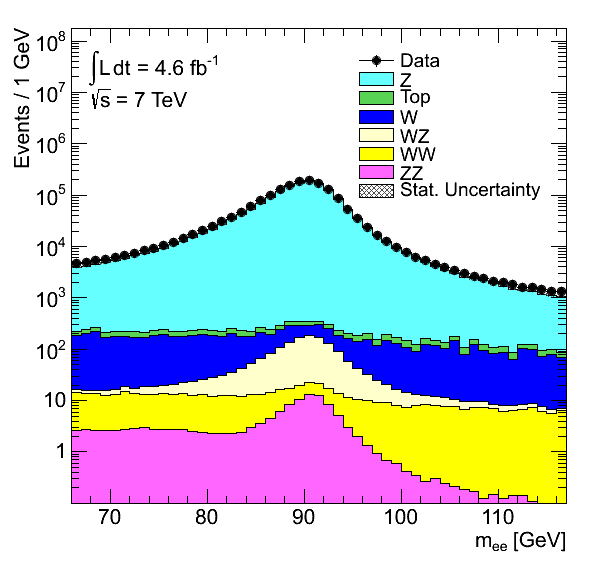
\includegraphics[width=0.47\textwidth]{Dilepton7TeV/AllE_Z_m}
        }
	\subfigure[]{
            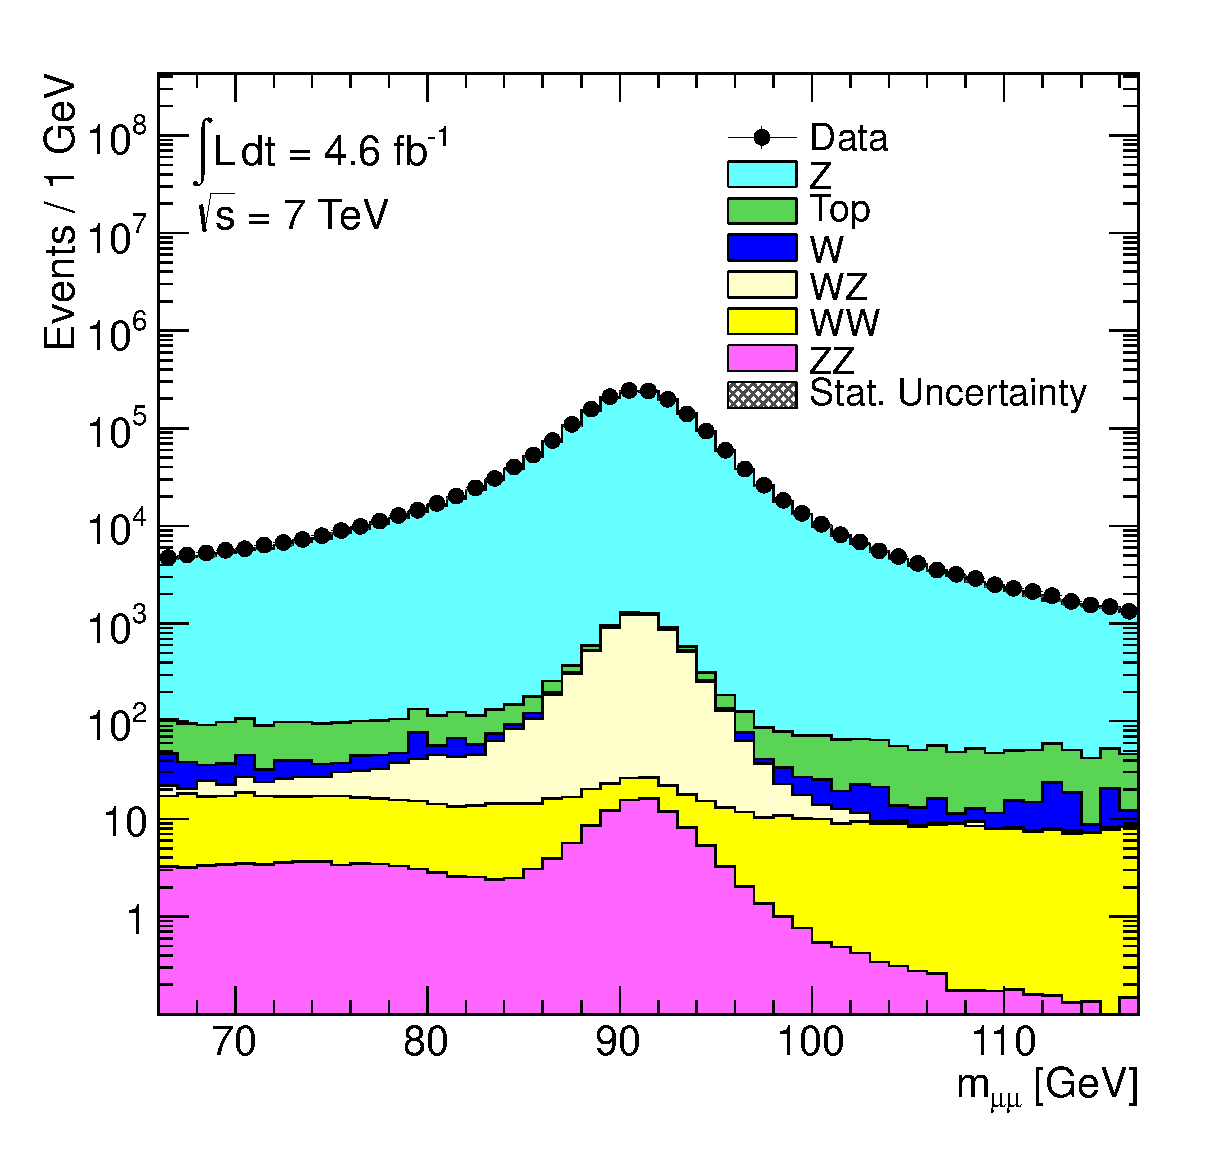
\includegraphics[width=0.47\textwidth]{Dilepton7TeV/AllMu_Z_m}
        }
	\subfigure[]{
            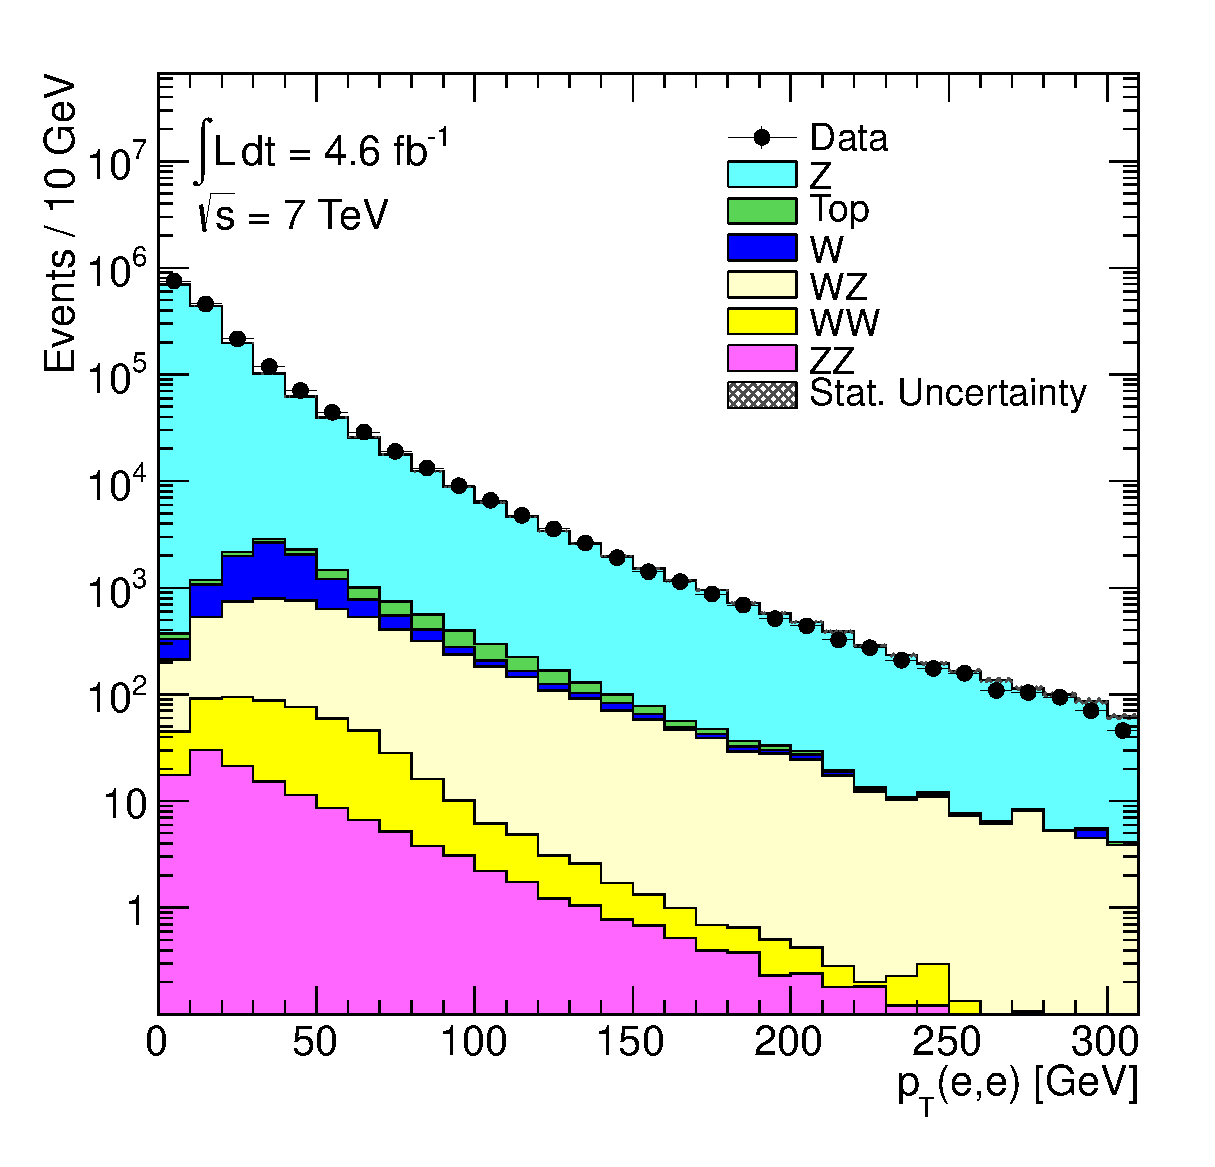
\includegraphics[width=0.47\textwidth]{Dilepton7TeV/AllE_Z_pt}
        }
	\subfigure[]{
            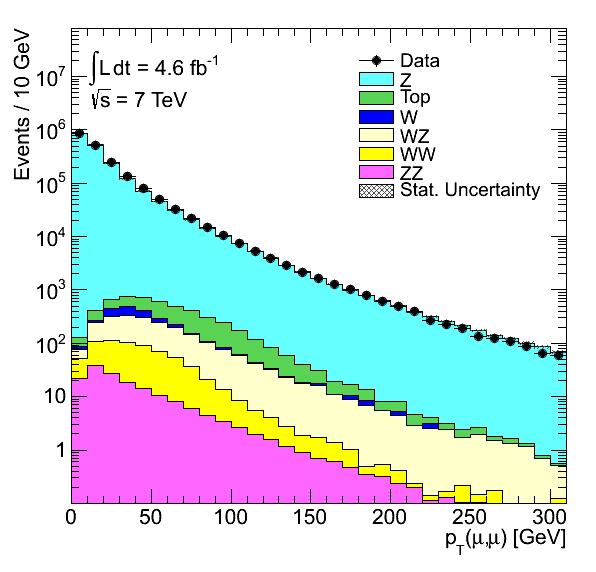
\includegraphics[width=0.47\textwidth]{Dilepton7TeV/AllMu_Z_pt}
        }
    \caption[Dilepton invariant mass and transverse momentum in the 7~\tev\
    data. ]
    {Figures (a) and (b) show distributions of the \dilepton\ invariant mass for \dielectron\ and 
     \dimuon\ pairs, respectively, in events in the 7~\tev\ data containing a pair of
    \ossf\ leptons passing all of the lepton selection criteria described
    in Sections~\ref{sec:objsel-el} and~\ref{sec:objsel-mu}. Figures (c) and (d) show the \dilepton\ transverse momentum for
    events passing the same criteria, with the additional requirement that the
    \dilepton\ pair have \sstooos. 
    }
\label{fig:dilep-mass-pt-seven}
\end{figure}

\begin{figure}[h]
\centering
	\subfigure[]{
            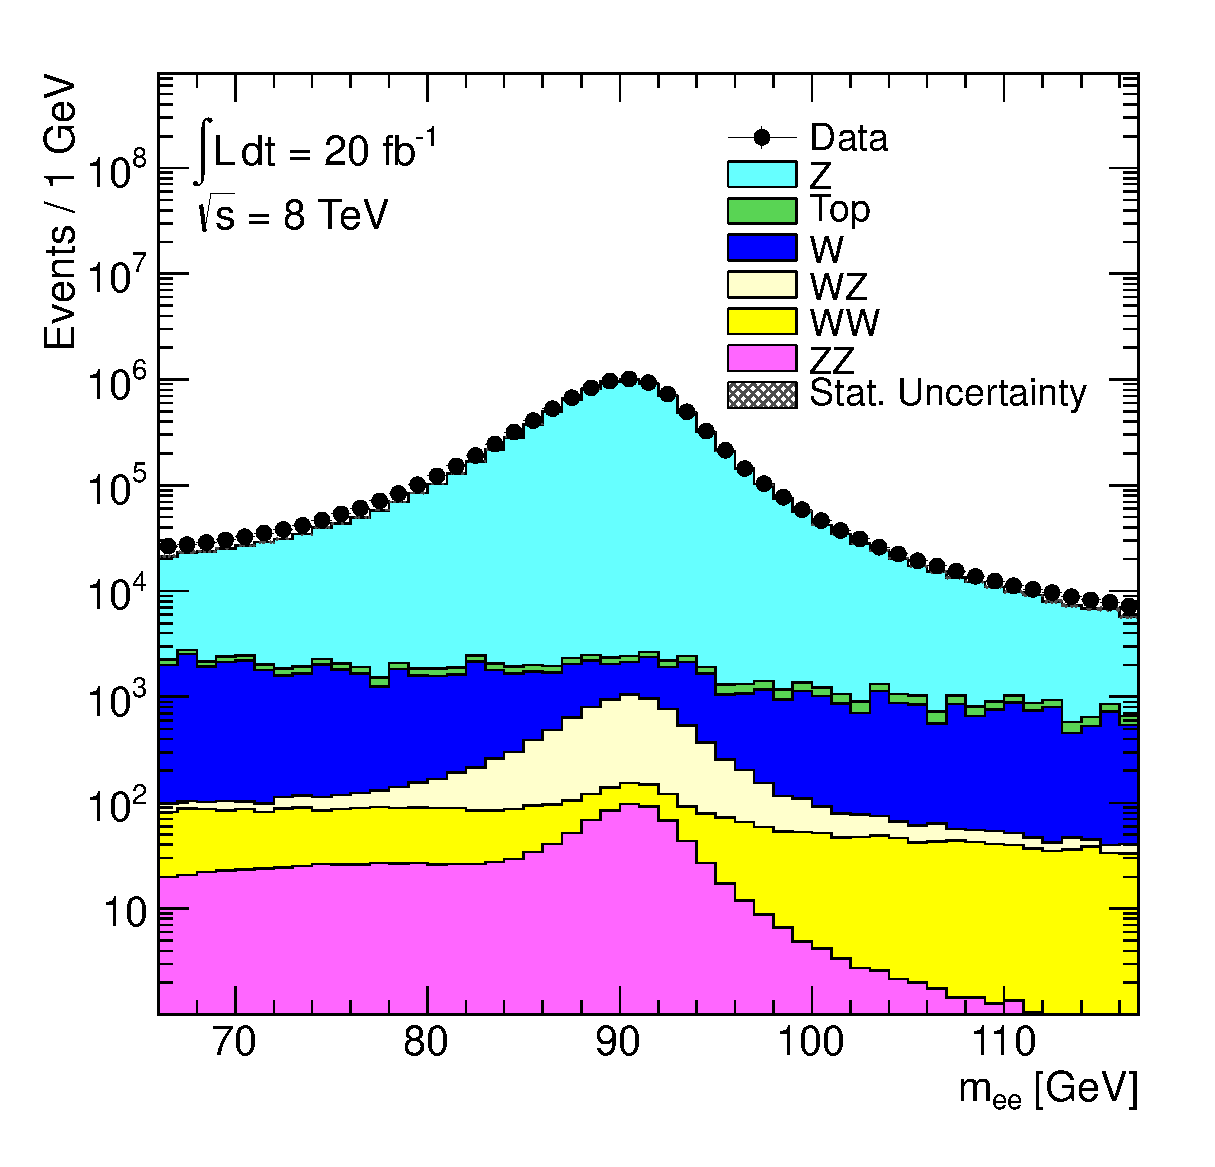
\includegraphics[width=0.47\textwidth]{Dilepton8TeV/AllE_Z_m}
        }
	\subfigure[]{
            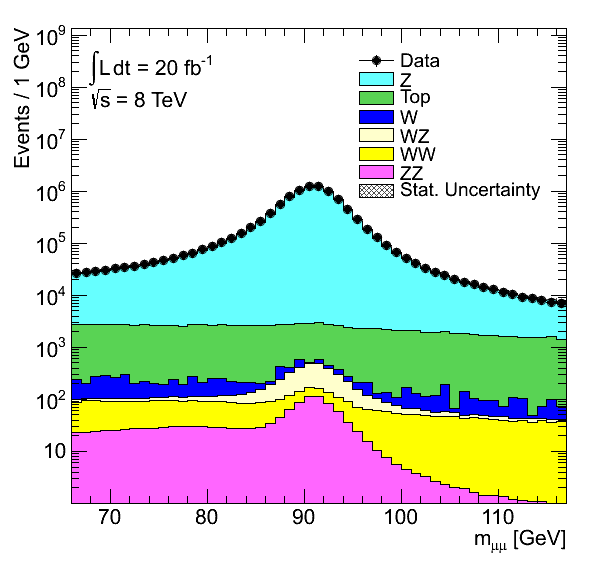
\includegraphics[width=0.47\textwidth]{Dilepton8TeV/AllMu_Z_m}
        }
	\subfigure[]{
            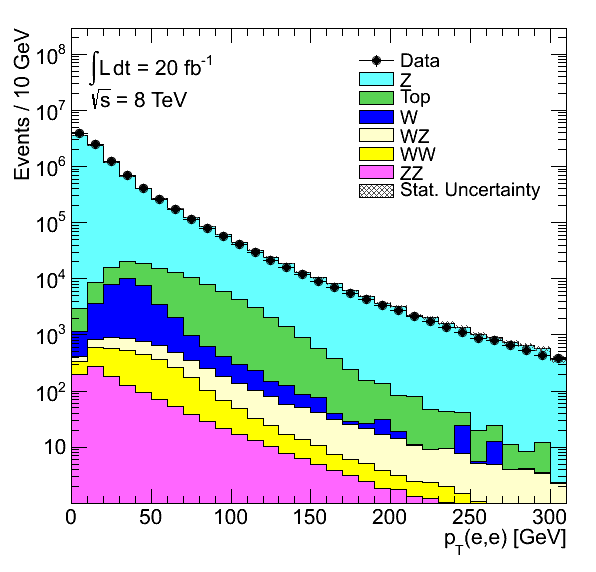
\includegraphics[width=0.47\textwidth]{Dilepton8TeV/AllE_Z_pt}
        }
	\subfigure[]{
            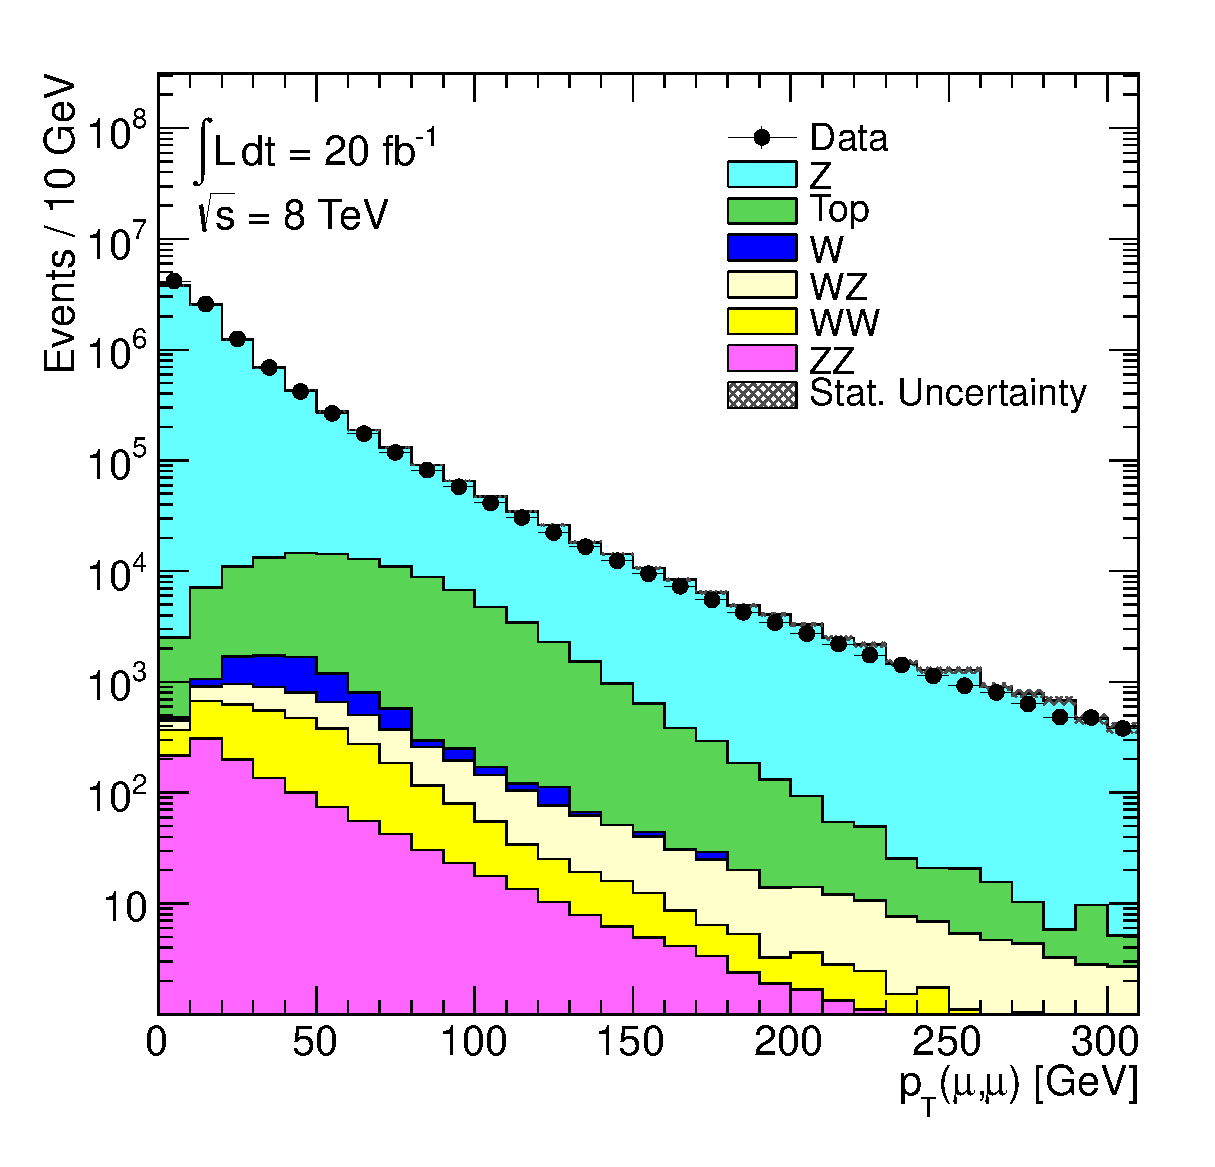
\includegraphics[width=0.47\textwidth]{Dilepton8TeV/AllMu_Z_pt}
        }
    \caption[Dilepton invariant mass and transverse momentum in the 8~\tev\
    data. ]
    {Figures (a) and (b) show distributions of the \dilepton\ invariant mass for \dielectron\ and 
     \dimuon\ pairs, respectively, in events in the 8~\tev\ data containing a pair of
    \ossf\ leptons passing all of the lepton selection criteria described
    in Sections~\ref{sec:objsel-el} and~\ref{sec:objsel-mu}. Figures (c) and (d) show the \dilepton\ transverse momentum for
    events passing the same criteria, with the additional requirement that the
    \dilepton\ pair have \sstooos. 
    }
\label{fig:dilep-mass-pt-eight}
\end{figure}

\begin{figure}[h]
\centering
\vspace{-5mm}
	\subfigure[]{
            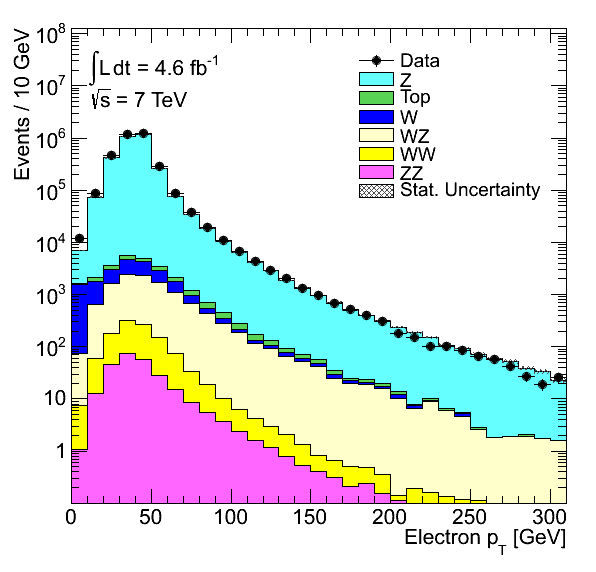
\includegraphics[width=0.47\textwidth]{Dilepton7TeV/AllE_lep_pt}
        }
	\subfigure[]{
            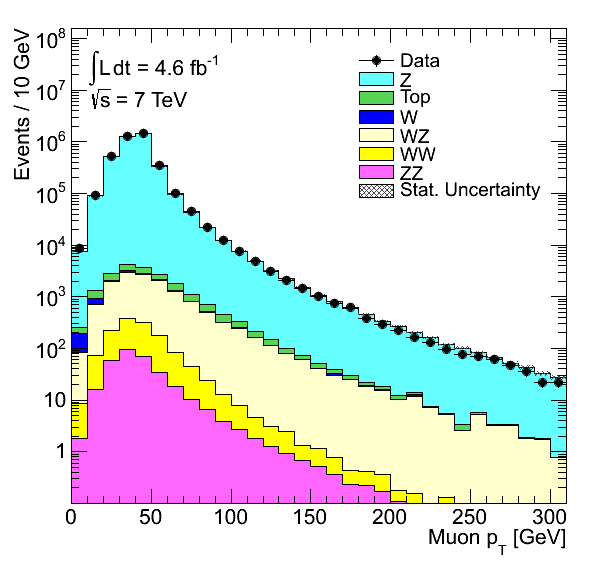
\includegraphics[width=0.47\textwidth]{Dilepton7TeV/AllMu_lep_pt}
        }
	\subfigure[]{
            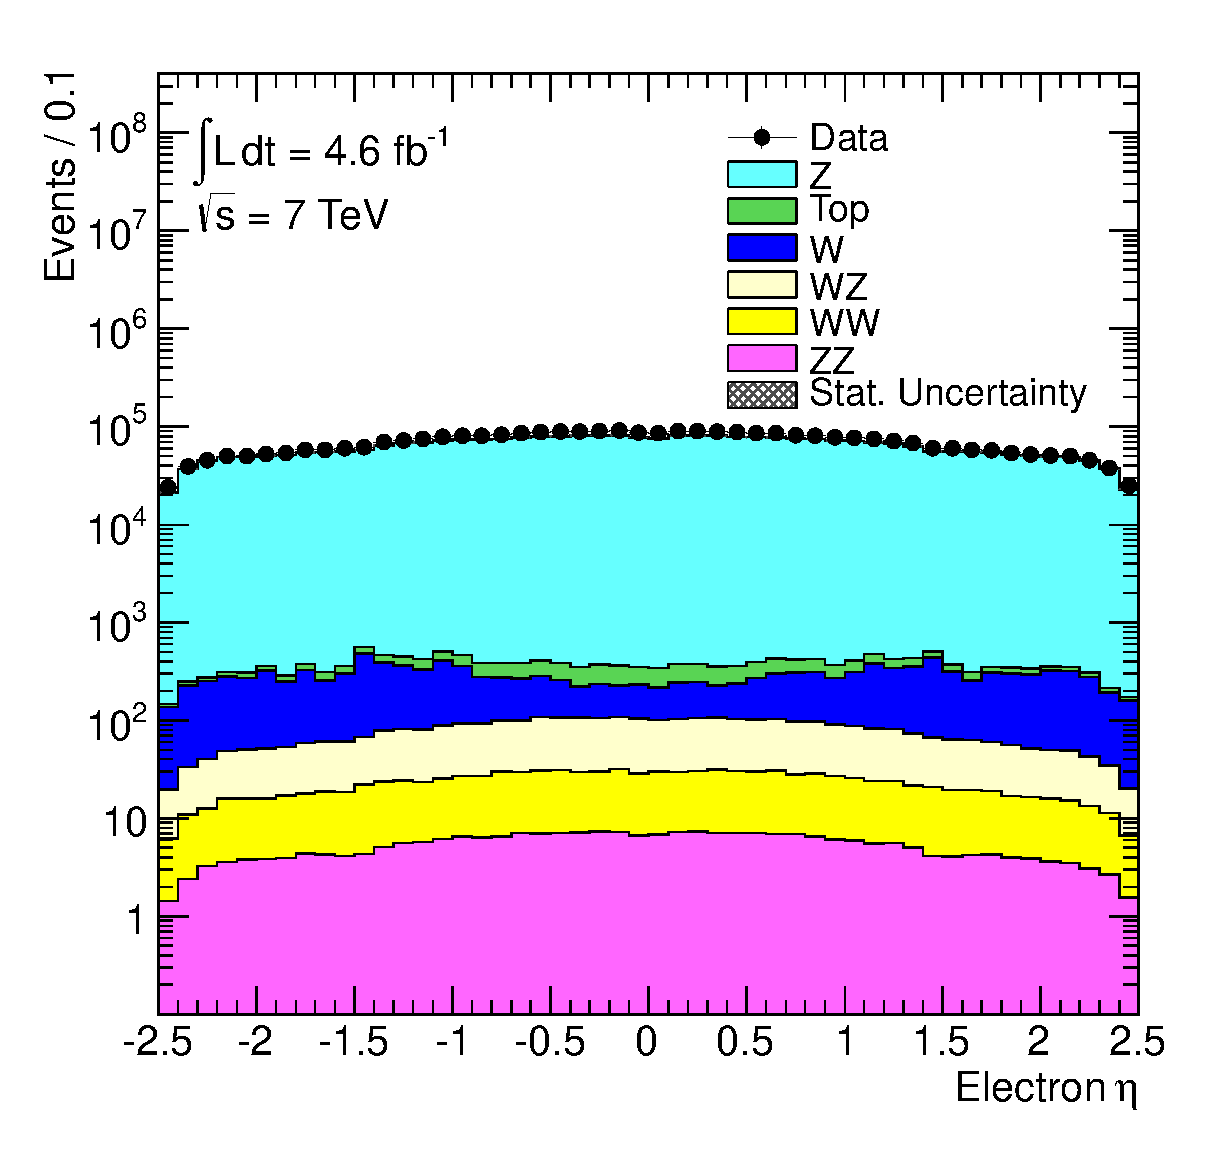
\includegraphics[width=0.47\textwidth]{Dilepton7TeV/AllE_lep_eta}
        }
	\subfigure[]{
            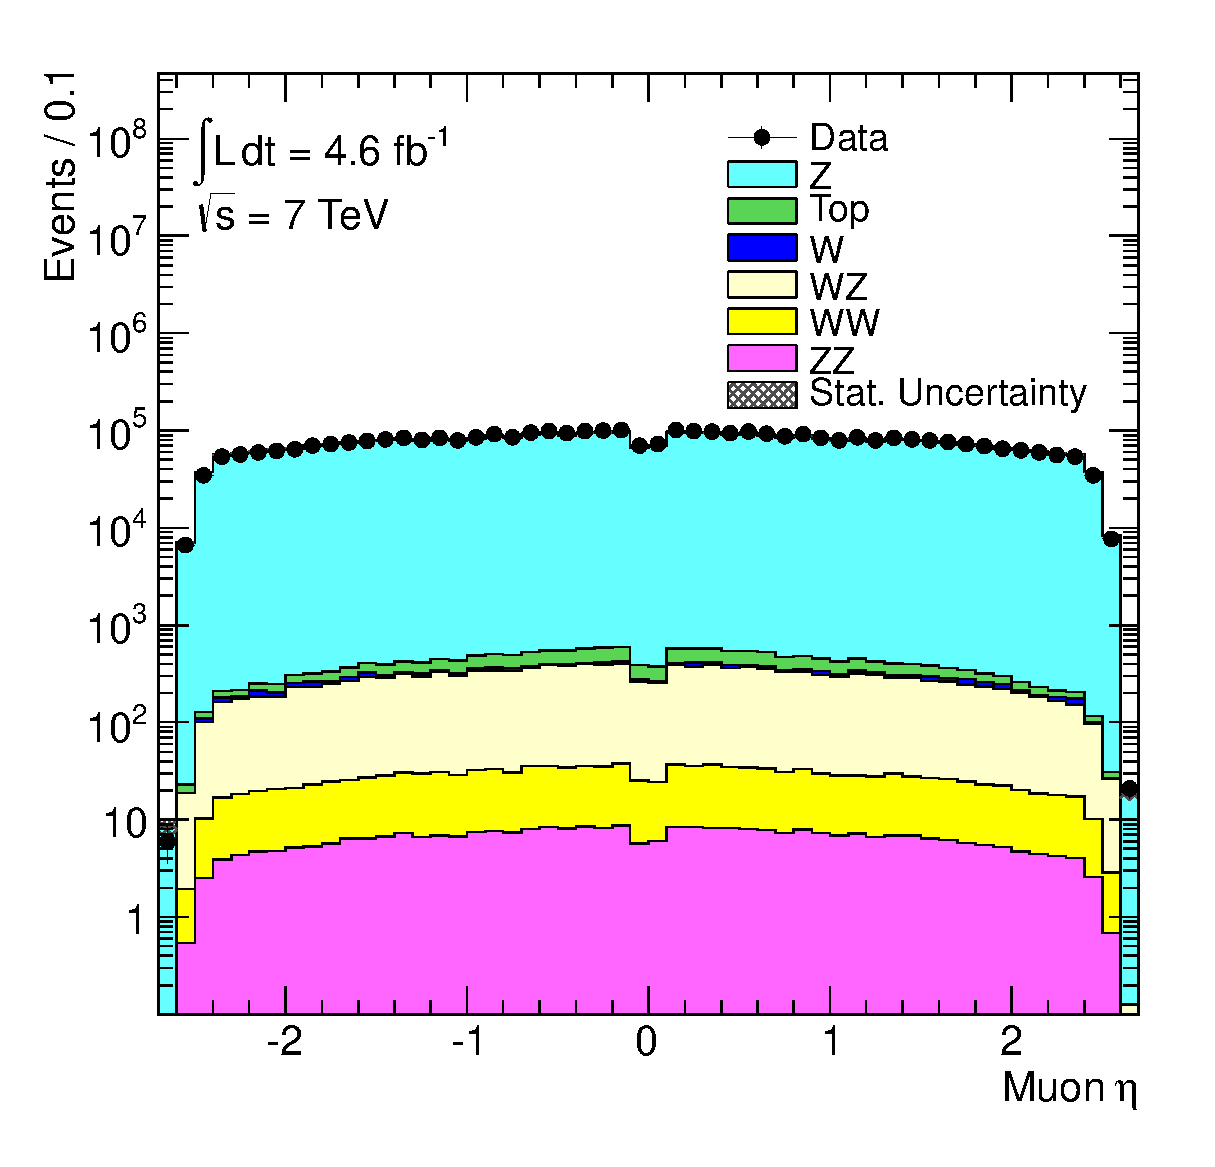
\includegraphics[width=0.47\textwidth]{Dilepton7TeV/AllMu_lep_eta}
        }
	\subfigure[]{
            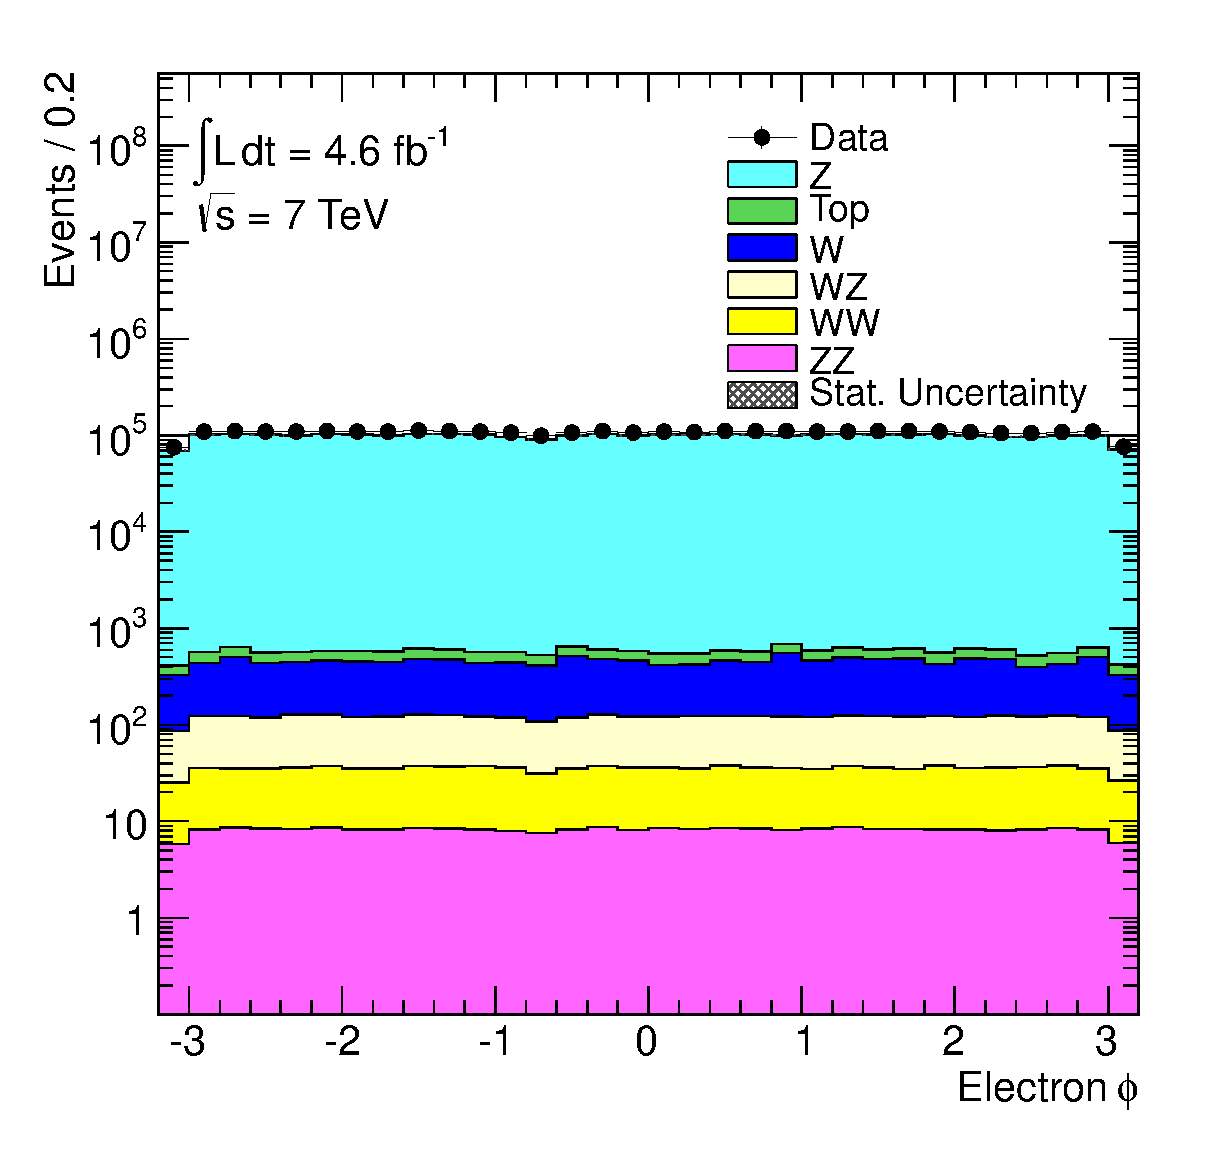
\includegraphics[width=0.47\textwidth]{Dilepton7TeV/AllE_lep_phi}
        }
	\subfigure[]{
            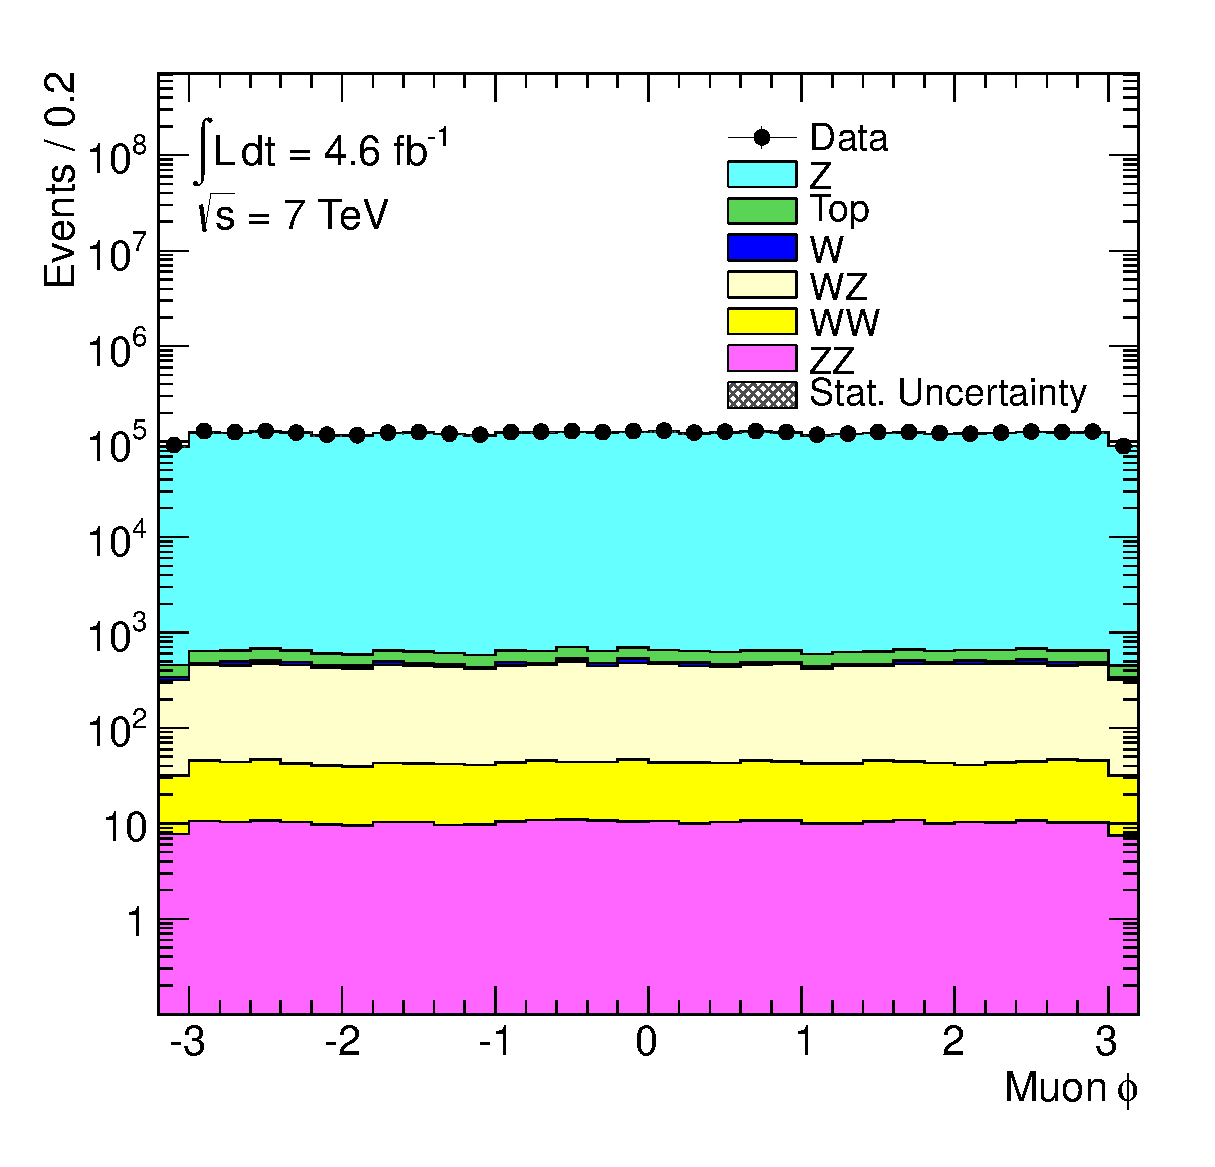
\includegraphics[width=0.47\textwidth]{Dilepton7TeV/AllMu_lep_phi}
        }
    \caption[Lepton kinematic distributions for \dilep\ events in the 7~\tev\
    data. ]
    {\small Kinematic distributions for leptons in events in the 7~\tev\
    data containing an \ossf\ lepton pair. The leptons are required to pass all of the selection
    requirements described in Sections~\ref{sec:objsel-el}
    and~\ref{sec:objsel-mu} and the pair must have \sstooos. 
    Figures (a) and (b) show the lepton \pt\ for electrons and muons
    respectively, figures (c) and (d) the lepton $\eta$ and figures (d) and (e)
    the lepton $\phi$.    }
\label{fig:dilep-lepkin-seven}
\end{figure}

\begin{figure}[h]
\centering
\vspace{-5mm}
	\subfigure[]{
            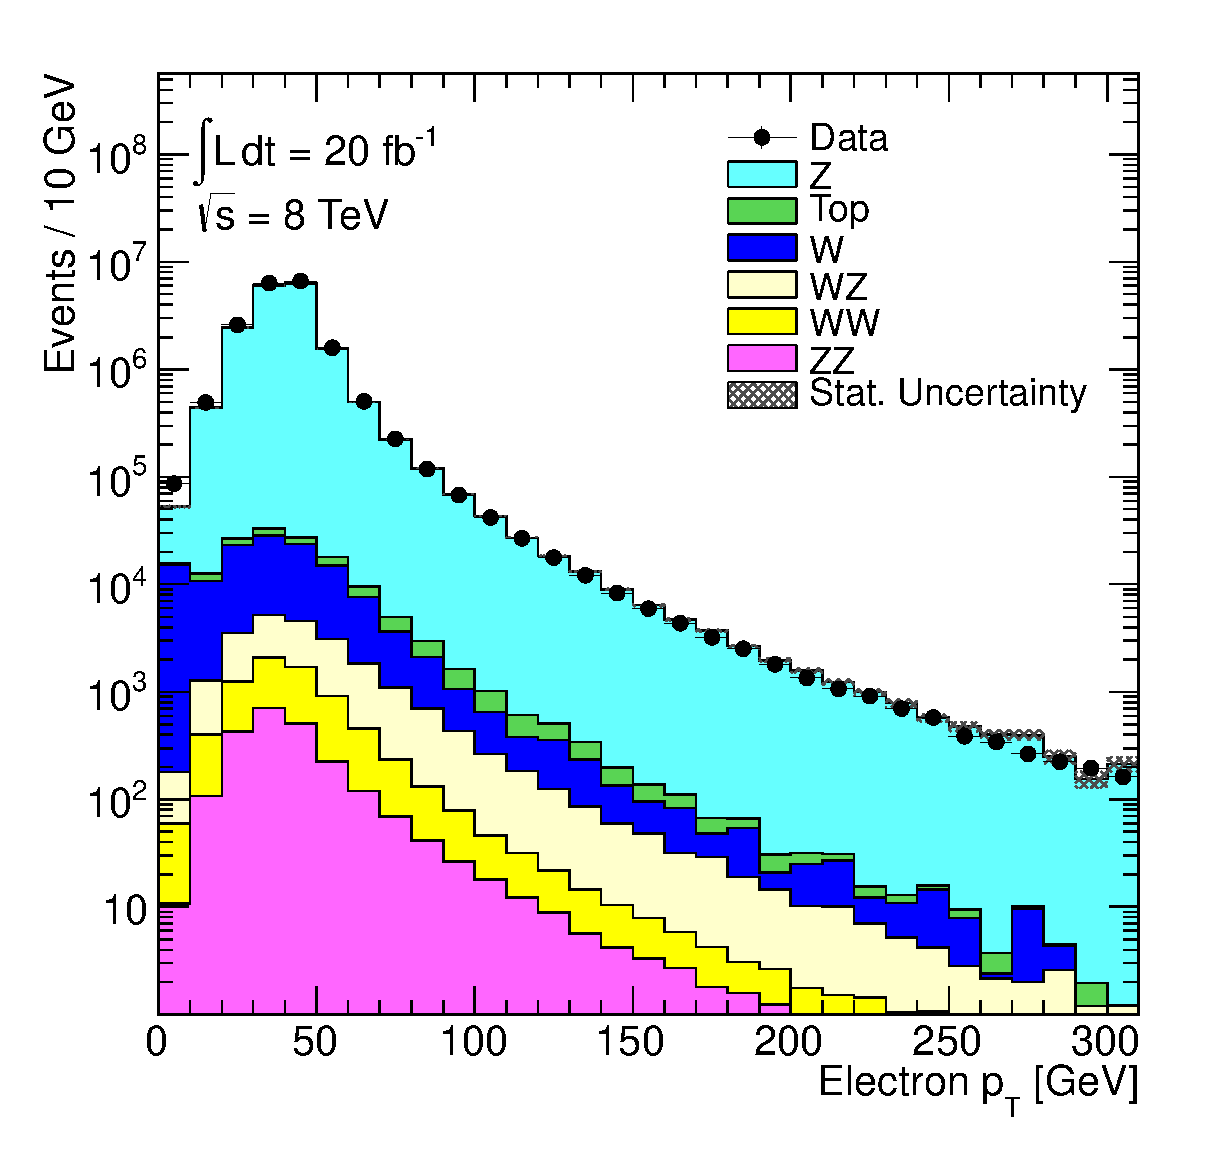
\includegraphics[width=0.47\textwidth]{Dilepton8TeV/AllE_lep_pt}
        }
	\subfigure[]{
            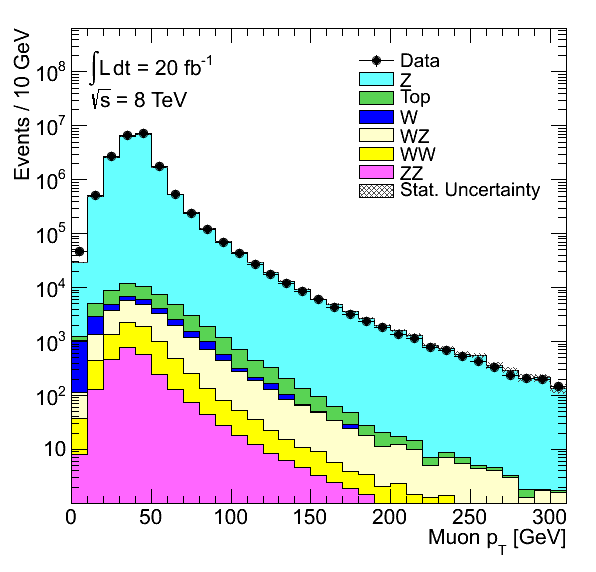
\includegraphics[width=0.47\textwidth]{Dilepton8TeV/AllMu_lep_pt}
        }
	\subfigure[]{
            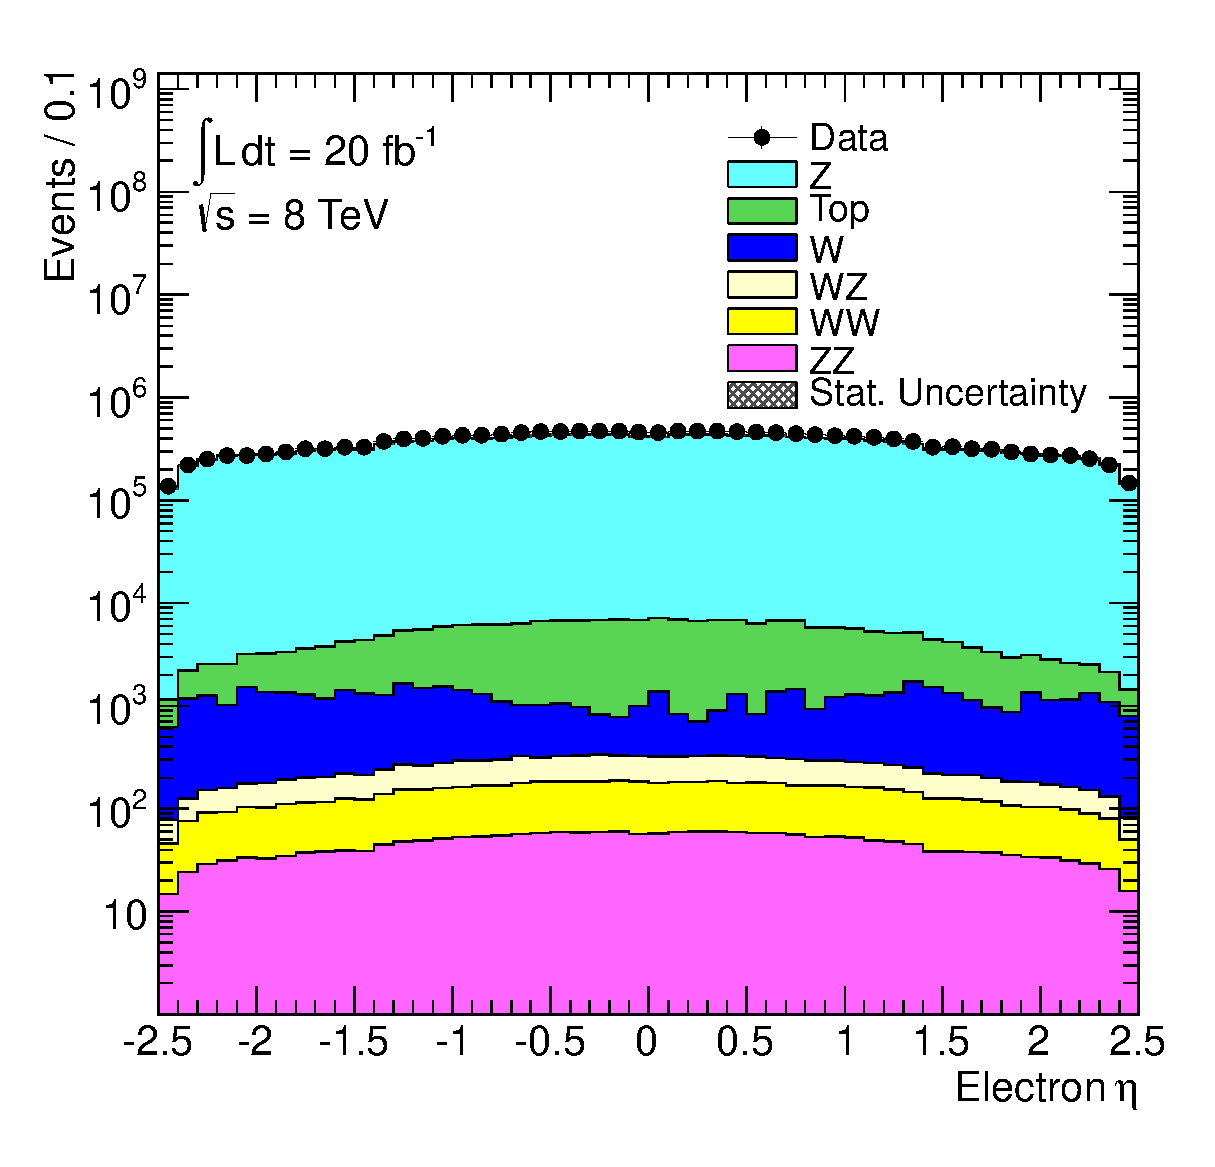
\includegraphics[width=0.47\textwidth]{Dilepton8TeV/AllE_lep_eta}
        }
	\subfigure[]{
            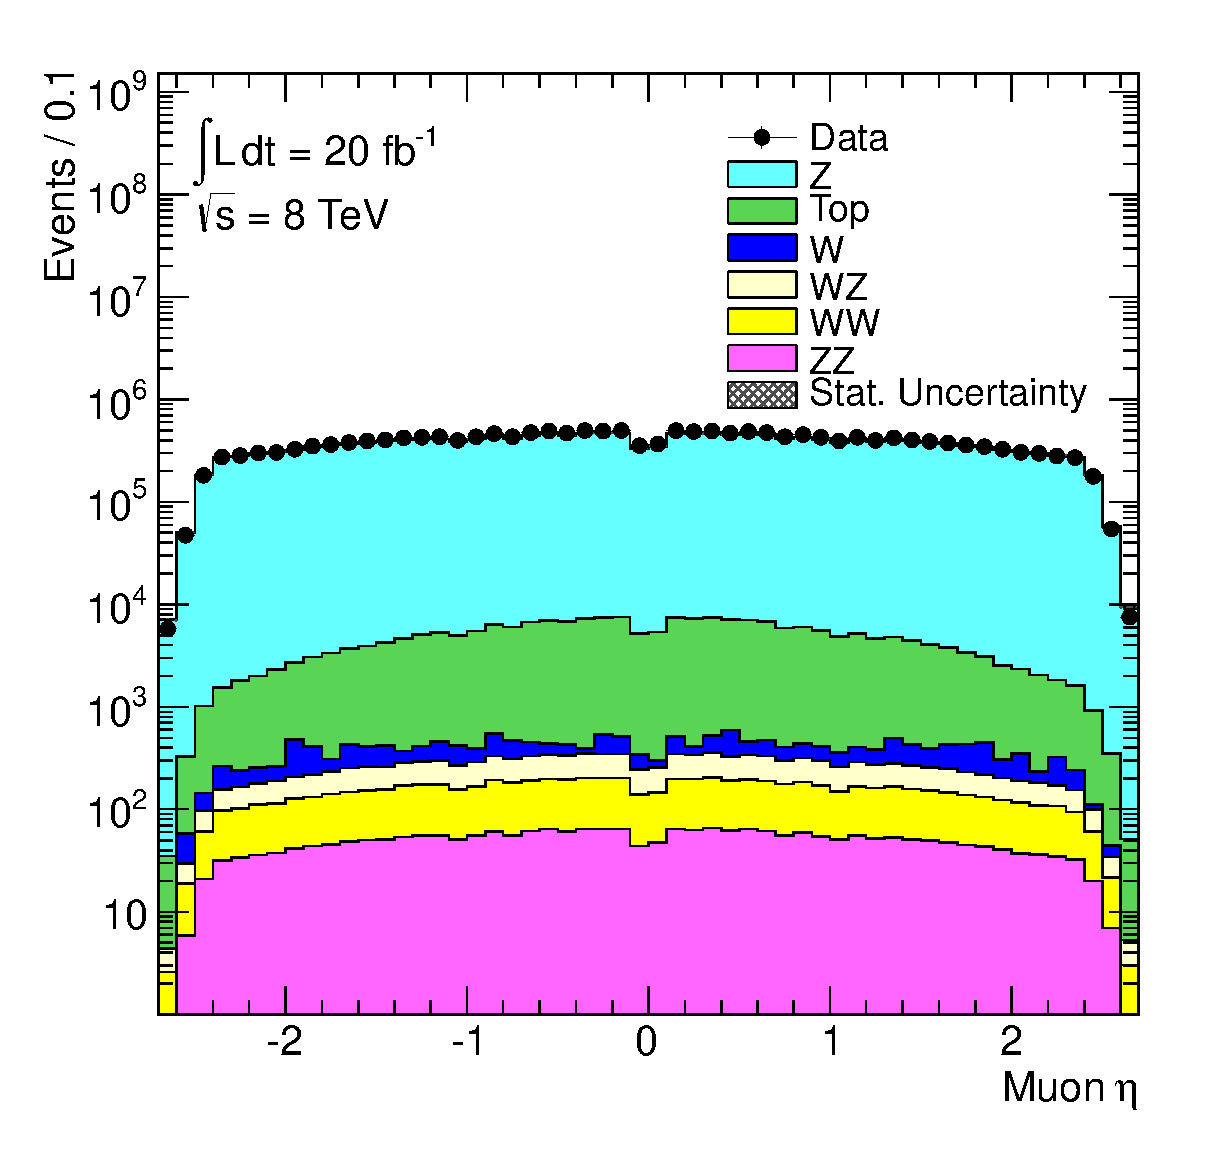
\includegraphics[width=0.47\textwidth]{Dilepton8TeV/AllMu_lep_eta}
        }
	\subfigure[]{
            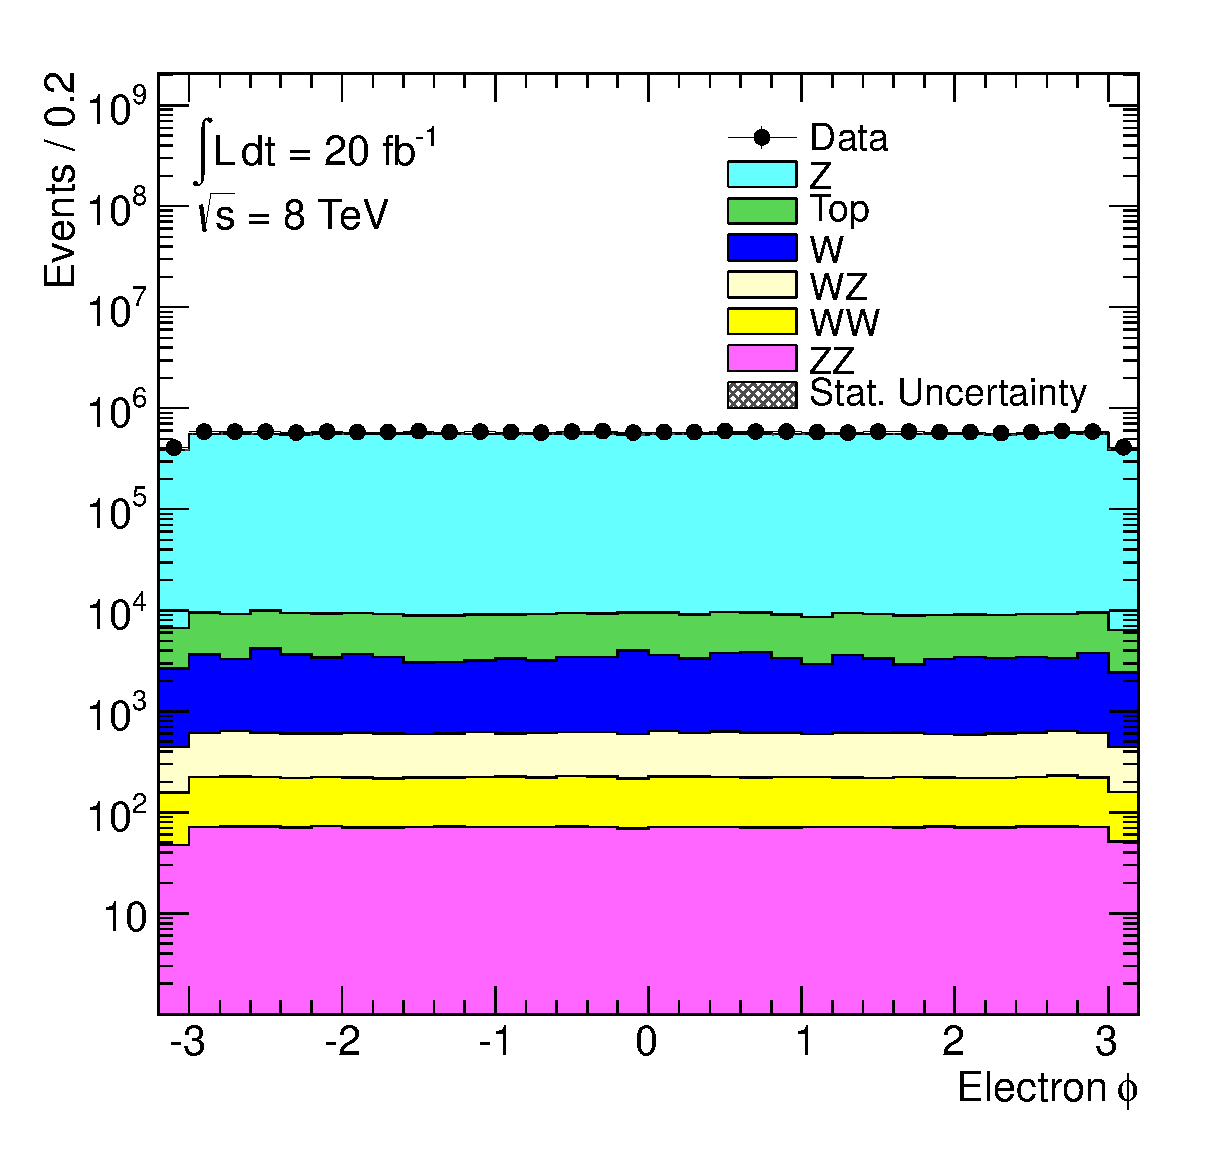
\includegraphics[width=0.47\textwidth]{Dilepton8TeV/AllE_lep_phi}
        }
	\subfigure[]{
            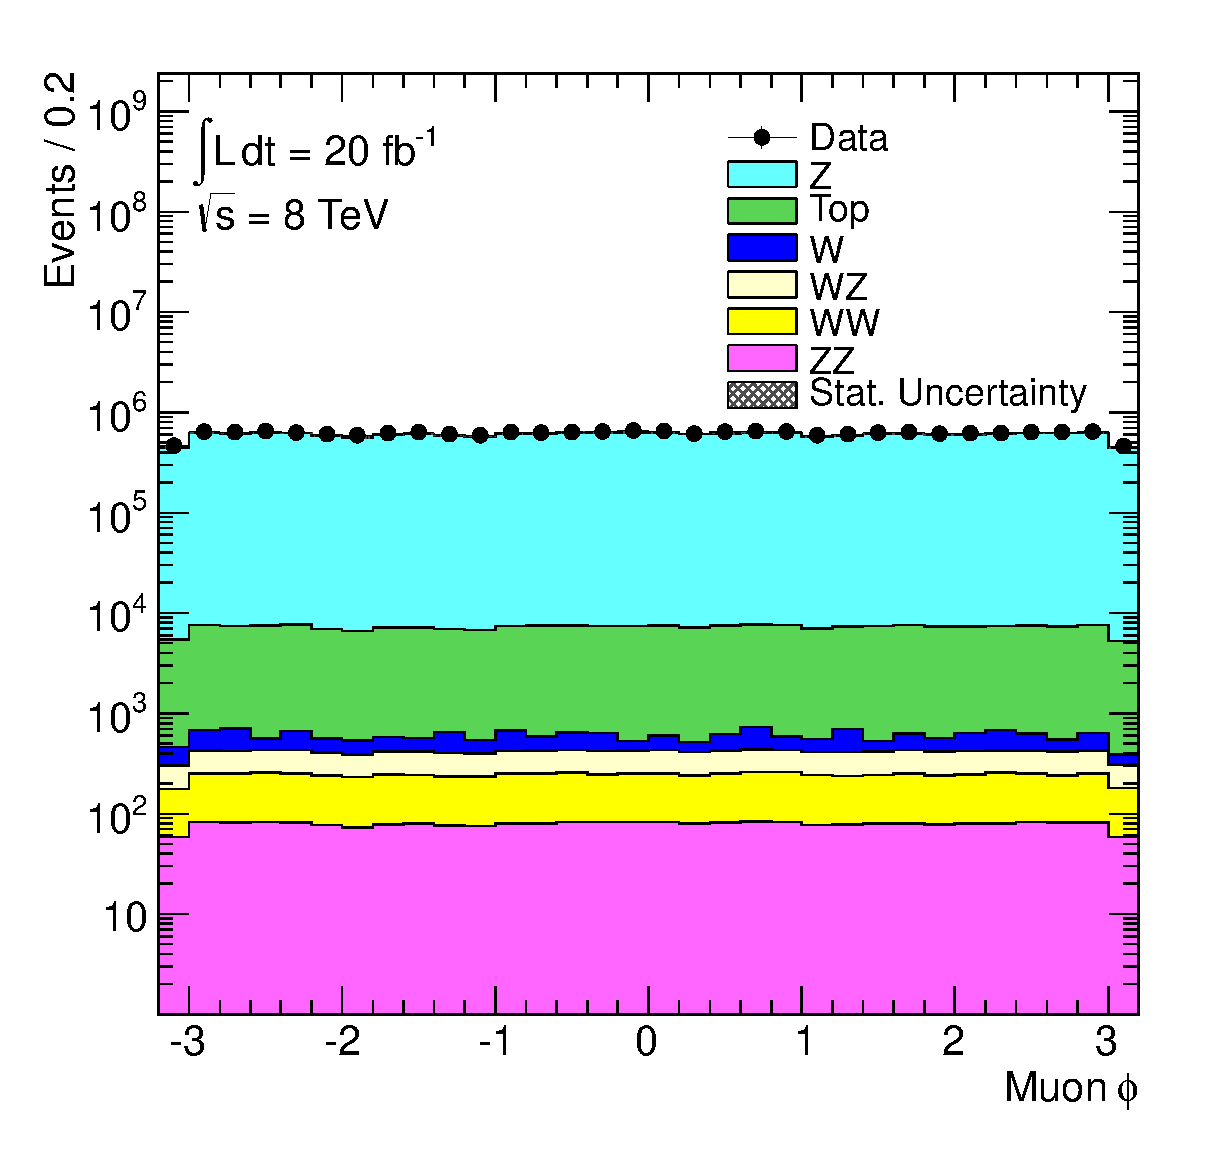
\includegraphics[width=0.47\textwidth]{Dilepton8TeV/AllMu_lep_phi}
        }
    \caption[Lepton kinematic distributions for \dilep\ events in the 8~\tev\
    data. ]
    {\small Kinematic distributions for leptons in events in the 8~\tev\
    data containing an \ossf\ lepton pair. The leptons are required to pass all of the selection
    requirements described in Sections~\ref{sec:objsel-el}
    and~\ref{sec:objsel-mu} and the pair must have \sstooos. 
    Figures (a) and (b) show the lepton \pt\ for electrons and muons
    respectively, figures (c) and (d) the lepton $\eta$ and figures (d) and (e)
    the lepton $\phi$.    }
\label{fig:dilep-lepkin-eight}
\end{figure}


\section{\ZZ\ Event Selection}
\label{sec:eventsel}

\subsection{\Z\ Candidate Definitions}

In referring to \Z\ candidate \dilep\ pairs, the following definitions are used:

\begin{itemize}

    \item {\bf Leading and Subleading:} The \Z\ candidate with the largest \pt\
    of the pair is referred to as the \intro{leading} \Z; the \Z\ candidate with the
    lower \pt\ is referred to as the \intro{subleading} \Z.

    \item {\bf Primary and Secondary:} The \Z\ candidate closest to the \Z\
    boson mass (from~\cite{PDG}) is referred to as the \intro{primary} \Z; the other
    candidate is referred to as the \intro{secondary} \Z.

\end{itemize}

%There is a strong correlation between the \pt\ of a \Z\ candidate and the
%closeness of its mass to the \Z\ mass, as seen
%in~\figs{data-zmass-zpt-seven}{data-zmass-zpt-eight}, so it is often, but not
%always, the case that the leading \Z\ candidate is also the primary \Z\
%candidate.

\subsection{Event Selection Requirements}

Candidate \ZZ\ events are selected by imposing the following requirements:

\begin{enumerate}

    \item {\bf Data Quality:} Events are required to pass a `Good Run List' to
    remove events occurring in a lumiblock where there were defects affecting
    the quality of the data; for example a ROD (Read Out Device) going `busy',
    meaning data from a large fraction of a sub-detector was missing.

    \item {\bf Trigger:} The event must pass a high \pt\ single electron or single
    muon trigger as described in~\sec{triggers}.

    \item {\bf Four leptons:} The event must have exactly four electrons or
    muons passing the selection requirements described in
    Sections~\ref{sec:objsel-el} and~\ref{sec:objsel-mu}. The requirement of
    exactly four leptons, rather than at least four leptons, greatly simplifies
    the background estimate. MC predicts that only
    1.3\% of signal events fail this cut. 
    In 7~\tev\ data, no events with more
    than four fully selected leptons were observed.
    In 8~\tev\ data, 11 events with more than four leptons passing all of the
    selection requirements were observed (without applying any mass
    requirements), compared to 1682 events with exactly four leptons.

    \item {\bf Lepton Separation:} The leptons are required to be spatially
    separated by $\Delta{R}(\ell,\ell)>0.2$. This requirement is automatically
    satisfied after applying the lepton isolation requirements (applied to all
    leptons except forward electrons). It is made here explicitly 
    % since it is important in the background estimate (see~\chap{bg}), and 
    to highlight the fact that there is no analysis sensitivity to events with
    leptons separated by \deltaRlt{0.2}, which is of importance when performing
    searches for nTGCs, where the \Z\ bosons are expected to be heavily boosted
    and thus the leptons produced at small opening angle the detector frame.
    The limits to sensitivity of this requirement ed is discussed below.

    \item {\bf Trigger match:} At least one selected lepton must match to the
    object that caused the trigger to fire, as described in~\sec{triggers}. 

    \item {\bf Quadruplet Formation:} There must be two same-flavour (SF),
    oppositely-signed (OS) lepton pairs. In $eeee$ and $\mu\mu\mu\mu$ events there are
    two possible ways of pairing the four leptons into OS pairs. The pairing which
    minimises the quantity $|m_{12}-m_{Z}|+|m_{34}-m_{Z}|$ is chosen, where
    $m_{12}$, $m_{34}$ are the invariant masses of the two lepton pairs in a certain
    pairing and $m_Z$ is the \Z\ boson mass, taken from~\cite{PDG}.

    \item {\bf ``Primary" \Z\ candidate:} The primary \Z\ candidate must satisfy the mass cut $66<m_{12}<116$~GeV.

    \item {\bf ``Secondary" \Z\ candidate:} Two non-exclusive mass cuts are
    applied to the secondary \Z\ candidate, one
    to select the event as a \ZZ\ event, the other to select the event as a
    \ZZs\ event:
      \begin{enumerate}
     \item To be classified as a \ZZ\ event, the secondary \Z\ candidate must satisfy
     the mass cut $66<m_{34}<116$~GeV.
     \item To be classified as a \ZZs\ event, the secondary \Z\ candidate
     must satisfy the mass cut $m_{34}>20$~GeV.
    \end{enumerate}
    For the 8~\tev\ data, only the \ZZ\ selection (selection (a)) is used.

    \item {\bf \JPsi\ Veto:} For the 8~\tev\ data, any events which have any
    combination of oppositely charged, same flavor lepton pairs with invariant
    mass below 5 GeV are rejected, in order to reject \JPsi\ events. This
    requirement was not applied for the 7~\tev\ data. The efficiency of this cut
    is estimated from \mc\ to be 96.6\%. No events failing this cut were
    observed in either the 7~\tev\ or the 8~\tev\ data.

\end{enumerate}

%Applying these requirements, a total
%of~\ZZSevenTeVNObsZZLLLL\ (\ZZSevenTeVNObsZZsLLLL) events
%are observed in the 2011 data for the \ZZ\ (\ZZs) selection. In the 2012 data, 
%~\ZZEightTeVNObsZZLLLL\ (\ZZEightTeVNObsZZsLLLL) events are
%observed for the \ZZ\ (\ZZs) selection. 

The expected number of events in
\LumiPassGRLTwentyEleven\ \ifb\ of 7~\tev\ data after various stages of the
selection is shown in~\tab{objSel-cutflow-seven}. The corresponding numbers for
\LumiPassGRLTwentyTwelve\ \ifb\ of 8~\tev\ data are shown
in~\tab{objSel-cutflow-eight}.

%%%%%%%%%%%%%%%%%%%%%%%%%%%%%
% Updated to 4.6fb-1 numbers for paper
% Nick, 25/5/2012
% No fwdEIso, fwd e, mu SF
%%%%%%%%%%%%%%%%%%%%%%%%%%%%%
\begin{table}[htbp]
	 \centering
         \small
	 \begin{tabular}{lcccc}
	 \hline\hline
%	 	 Cutflow & \multicolumn{4}{|c|}{Number of Events} \\ \cline{2-5}
$N_{ZZ}$ (7~\tev, \LumiPassGRLTwentyEleven\ \ifb)	  & \eeee\ & \mmmm\ & \eemm\ & \llll\  \\
	 	 \hline
   Four leptons             &  15.23 $\pm$ 0.17 &  25.49 $\pm$ 0.23  &  41.55 $\pm$ 0.31 &  82.27 $\pm$ 0.43  \\ 
   %Trigger Match           &  15.01 $\pm$ 0.17 &  24.93 $\pm$ 0.23  &  40.69 $\pm$ 0.31 &  80.66 $\pm$ 0.41   \\ 
   Quadruplet               &  14.51 $\pm$ 0.17 &  24.92 $\pm$ 0.23  &  39.98 $\pm$ 0.29 &  79.41 $\pm$ 0.41   \\ 
   66$<M_{01}<$166~\gev\    &  12.92 $\pm$ 0.16 &  21.60 $\pm$ 0.22  &  34.67 $\pm$ 0.28 &  69.21 $\pm$ 0.38   \\ 
   66$<M_{34}<$116~\gev\    &  12.51 $\pm$ 0.15 &  20.35 $\pm$ 0.21  &  32.50 $\pm$ 0.27 &  65.37 $\pm$ 0.37   \\ 
   $M_{34}>$20~\gev\        &  10.28 $\pm$ 0.14 &  16.45 $\pm$ 0.19  &  26.67 $\pm$ 0.24 &  53.41 $\pm$ 0.34   \\

	 \hline\hline
	 \end{tabular}
           \caption[Expected number of events in the 7~\tev\ data by cut for
           \LumiPassGRLTwentyEleven\ \ifb.]{Expected number of events in the 7~\tev\ data by cut for
           \LumiPassGRLTwentyEleven\ \ifb. The errors are statistical only. The
           contribution from $\ZZ \to \tau+X$ where the tau decays into an
           electron or a muon is included; the estimated contribution is given
           in~\tab{objSel-czz-seven}.}
          \label{table:objSel-cutflow-seven}
\end{table}

\begin{table}[htbp]
	 \centering
         \small
	 \begin{tabular}{lcccc}
	 \hline\hline
%	 	 Cutflow & \multicolumn{4}{|c|}{Number of Events} \\ \cline{2-5}
$N_{ZZ}$ (8~\tev, \LumiPassGRLTwentyTwelve\ \ifb)	  & \eeee\  & \mmmm\ & \eemm\ & \llll\ \\
	 	 \hline

         Four leptons &  $106.95 \pm 0.62$ &  $167.39 \pm 0.80$ &  $266.62 \pm 1.42$ &  $540.97 \pm 1.75$ \\
          Quadruplet &  $102.43 \pm 0.61$ &  $167.27 \pm 0.80$ &  $260.76 \pm 1.41$ &  $530.47 \pm 1.73$ \\
     66$<M_{01}<$166 &  $82.65 \pm 0.55$ &  $132.07 \pm 0.71$ &  $205.55 \pm 1.25$ &  $420.27 \pm 1.54$ \\
     66$<M_{34}<$116 &  $59.63 \pm 0.46$ &  $90.97 \pm 0.59$ &  $143.02 \pm 1.05$ &  $293.62 \pm 1.29$ \\
        %Trigger Match &  $59.62 \pm 0.46$ &  $90.33 \pm 0.59$ &  $142.79 \pm 1.04$ &  $292.74 \pm 1.29$ \\
            \JPsi\ Veto &  $59.53 \pm 0.46$ &  $90.23 \pm 0.59$ &  $142.71 \pm 1.04$ &  $292.47 \pm 1.28$ \\
                %NoSf &  $64.77 \pm 0.50$ &  $93.33 \pm 0.61$ &  $151.34 \pm 1.11$ &  $309.44 \pm 1.36$ \\
              %M34>20 &  $73.72 \pm 0.52$ &  $114.46 \pm 0.66$ &  $175.26 \pm 1.16$ &  $363.45 \pm 1.43$ \\

	 \hline\hline
	 \end{tabular}
           \caption[Expected number of events in the 8~\tev\ data by cut for
           \LumiPassGRLTwentyTwelve\ \ifb.]{Expected number of events in the 8~\tev\ data by cut for
          \LumiPassGRLTwentyTwelve\ \ifb. The errors are statistical only. The
           contribution from $\ZZ \to \tau+X$ where the tau decays into an
           electron or a muon is included; the estimated contribution is given
           in~\tab{objSel-czz-eight}.}
          \label{table:objSel-cutflow-eight}
\end{table}

\section{Selection Efficiencies}

\subsection{Mis-pairing Rates}
\label{sec:mispairing}

As described above, in \eeee\ and \mmmm\ final states there are two possible
ways of pairing the four leptons to give two oppositely signed pairs. There are
a number of different ways of resolving this ambiguity, using different pairing
algorithms. All pairing algorithms will have some rate of failure, so it is
important to find the algorithm with the lowest mis-pairing rate.

The mis-pairing rates of four algorithms were compared. The four algorithms
considered were:

\begin{enumerate}
    \item {\bf Sum Of Distances:} Choose the pairing minimising the quantity
    ${|m_{12}-m_{Z}|+|m_{34}-m_{Z}|}$.
    \item {\bf Sum Of Distances Squared:} Choose the pairing minimising the quantity
    $(m_{12}-m_{Z})^{2}+(m_{34}-m_{Z})^{2}$.
    \item {\bf Closest to the pole:} Choose the pairing which has the closest
    \dilep\ pair to the \Z\ mass.
    \item {\bf Breit Wigner Probability:} For each pairing calculate the product
    of the values of two Breit Wigner probability distributions centred at the \Z\ mass with
    width equal to the \Z\ width evaluated at the masses of the two \dilep\
    pairs and choose the pairing with the highest probability.
\end{enumerate}

The mis-pairing rates of each algorithm are estimated using \ZZeemm\ events, by
assigning \dilep\ pairs using the algorithm in question ignoring
lepton flavour, then checking whether the
pairing chosen by the algorithm is the correct one by checking whether the
chosen pairing has same-flavour pairs.
The mis-pairing rates estimated in this way are given in~\tab{mis-pairing}. The
rates are calculated after applying the \Z\ mass cuts based on the correct
pairing. For
\ZZ\ events, the `Sum Of Distances' algorithm has the lowest mis-pairing rate of
1.1\%.
For \ZZs\ events that are not \ZZ\ events (i.e. one of the \dilep\ pairs is
outside \sstooos), the mis-pairing rates are significantly higher, and for these
events the  `Sum Of Distances' algorithm has a mis-pairing rate of 22.5\%. In
this case the `Closest to the pole' algorithm gives the lowest mis-pairing rate.
Considering the full \ZZs\ selection, the `Breit-Wigner' algorithm gives the
lowest mis-pairing rate, with the `Sum Of Distances' coming second.

\begin{table}[htbp]
\small
    \centering
    \begin{tabular}{l c c c}
    %\begin{tabular}{p{3cm}p{1.2cm}p{1.2cm}p{1.2cm}p{1.2cm}}
	\hline\hline
        Algorithm                   & \ZZ\ (\%)     & \ZZs\ (\%)    & \ZZs\ not \ZZ (\%)  \\
        \hline
        Sum Of Distances            & 1.1 $\pm$ 0.1 & 4.7 $\pm$ 0.2 & 22.5 $\pm$ 0.8 \\
        Sum Of Distances Squared    & 1.3 $\pm$ 0.1 & 6.6 $\pm$ 0.2 & 33.6 $\pm$ 1.0 \\
        Closest to Pole             & 5.1 $\pm$ 0.2 & 5.5 $\pm$ 0.2 & \phantom{0}7.7  $\pm$ 0.5 \\
        Breit Wigner Probability    & 1.4 $\pm$ 0.1 & 2.9 $\pm$ 0.1 & 10.7 $\pm$ 0.6 \\
        \hline\hline
    \end{tabular}
    \caption{Mis-pairing rates in percent for different algorithms for choosing the
    \dilep\ pairs in \fourlep\ events. The errors shown are due to \mc\ statistics.}
    \label{table:mis-pairing}
\end{table}

In practice, it is not possible to apply different algorithms to the \ZZ\ and
\ZZs\ selections, since until one has chosen a pairing it is not possible to
apply mass cuts and thus not possible to decide whether the event is \ZZ\ or
\ZZs. The `Sum of Distances' algorithm is thus applied to all events, since it
gives the lowest mis-pairing for \ZZ\ events.

\subsection{Effect of Minimum \deltaR\ Requirement}

As discussed above, the lepton isolation requirements prevent any event with
leptons overlapping with \deltaRlt{0.2} from passing
the selection, since the lower \pt\ lepton would be vetoed by the
energy of the higher \pt\ lepton in its isolation cone, and the event would fail
the selection as it would not have four selected leptons. In events with low
\pt\ \Z\ bosons this does not affect the efficiency significantly since in the
\Z\ boson rest frame the leptons are produced `back-to-back'. In events with
highly boosted \Z\ bosons the leptons are produced with small opening angle in
the detector frame, and so the \deltaR\ requirement imposes an upper threshold on the centre of mass energy to
which the analysis is sensitive.

~\fig{objSel-deltaRcutoff} shows the minimum \deltaR\ between any two leptons
at generator level in \fourlep\ events as a function of the
mass of the \fourlep\ system and as a function of the transverse momentum of the
leading \Z. A \ZZllll\ \mc\ sample generated with aTGCs is used, with the
anomalous coupling \ffourg\ set to 0.4
and no form-factor applied, in order to give statistics at high centre of mass
energies. The plots show that the \deltaRlt{0.2} cut limits sensitivity to
events with $\mZZ>2$~\tev\ and to events with $\pt(Z1)>900$~\gev.

\begin{figure}[h]
\centering
	\subfigure[]{
            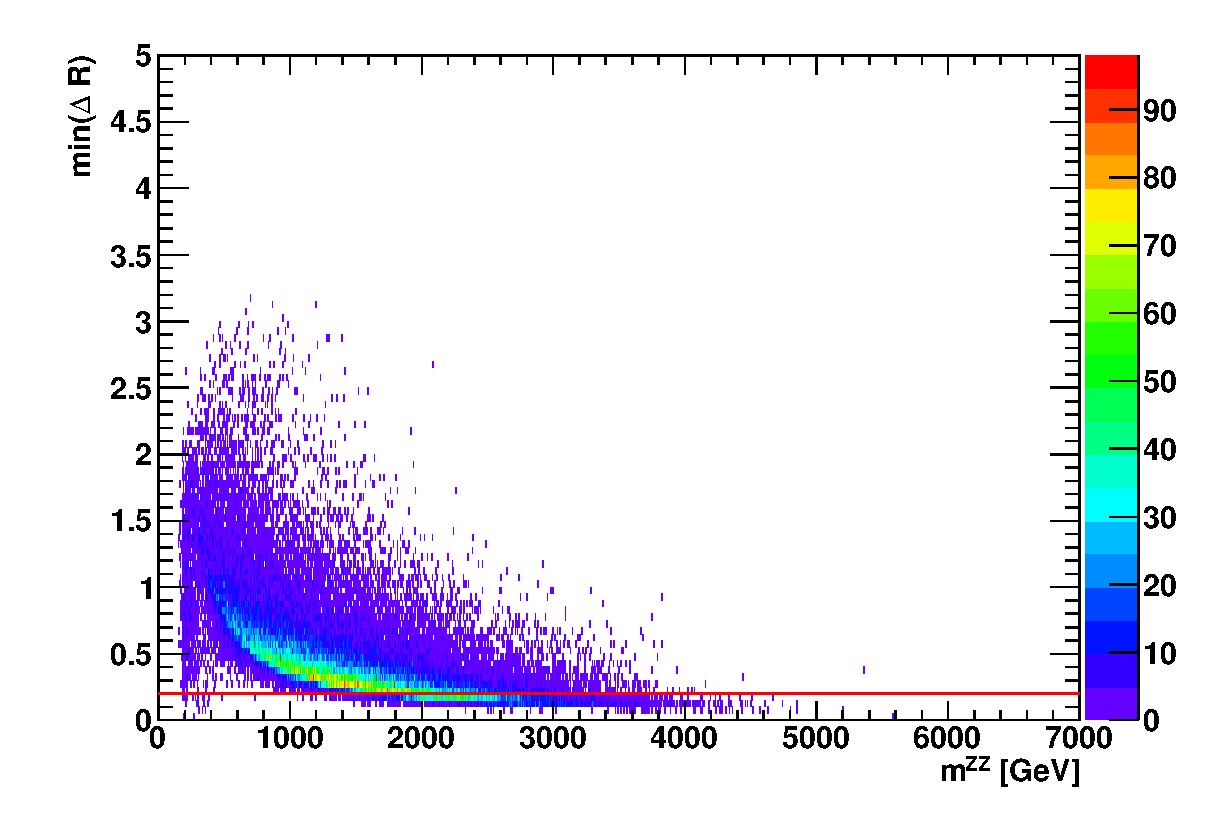
\includegraphics[width=0.7\textwidth]{deltaRcutoffs/truth_fidZZ_mzz_minDR_TGC_F4G0p4_n0}
        }
	\subfigure[]{
            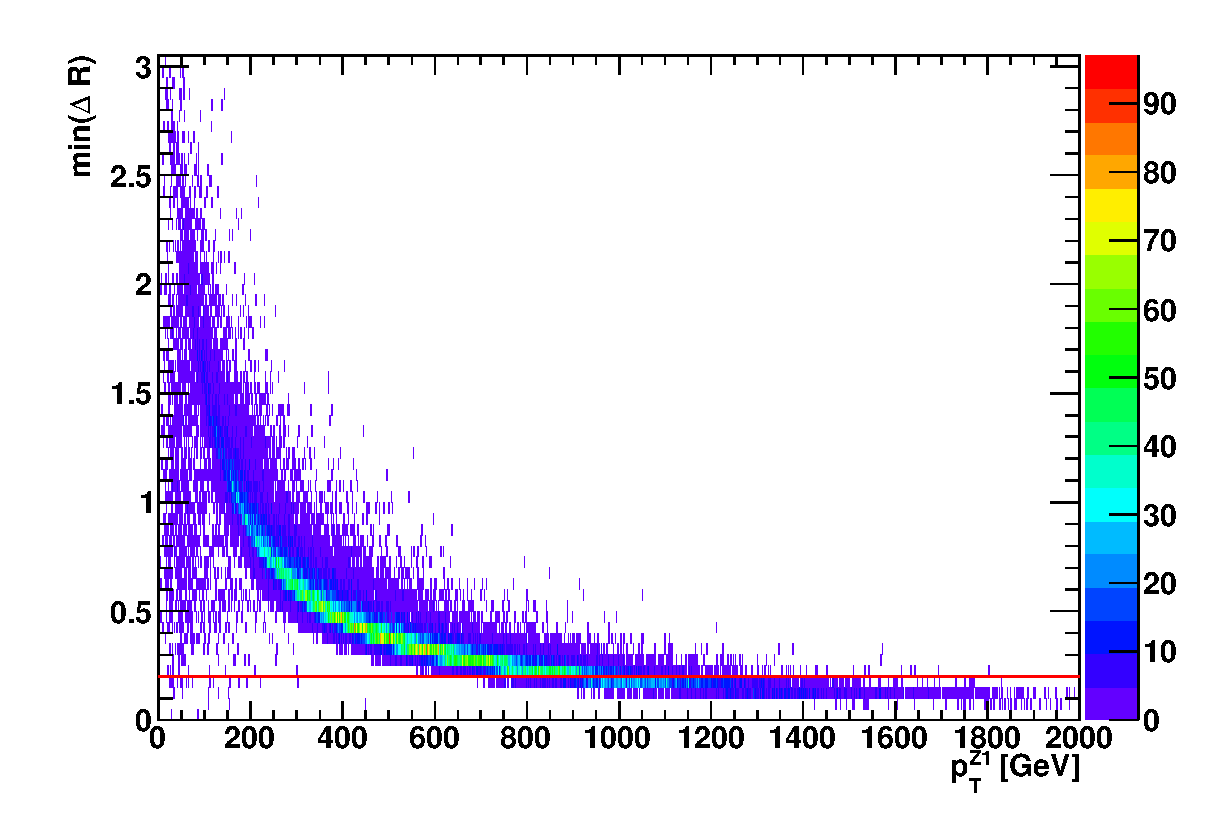
\includegraphics[width=0.7\textwidth]{deltaRcutoffs/truth_fidZZ_ptz1_minDR_TGC_F4G0p4_n0}
        }
    \caption[Effect of the \deltaRlt{0.2} requirement on sensitivity to boosted
    \fourlep\ systems.]{The minimum \deltaR\ between any two leptons at
    generator level in a \fourlep\
    \mc\ sample as a function of (a) mass of the
    \fourlep\ system and (b) transverse momentum of the leading \Z. A \ZZllll\
    sample generated with aTGCs is used, with $\ffourg=0.4$ and no form-factor
    applied, in order to give statistics at high centre
    of mass energies. The
    horizontal red line shows the \deltaRlt{0.2} cut. }
\label{fig:objSel-deltaRcutoff} 
\end{figure}

\subsection{Reconstruction Acceptance \CZZ}
\label{sec:objSel-CZZ}

In order to extrapolate from the number of observed events to a \cx\ or similar
measurement, it is necessary to know the acceptance of the selection
requirements. This is described by the \intro{reconstruction acceptance factor,
\CZZ}. Formally, this is defined as:

\begin{equation}
C_{ZZ}= \epsilon_{trig} \times \epsilon_{event} \times \epsilon_{lep} \times \alpha_{reco}
\end{equation}
where $\epsilon_{trig}$ is the trigger efficiency, $\epsilon_{event}$ is 
the efficiency of the event level cuts, and
$\epsilon_{lep} =\epsilon_{lep1}\epsilon_{lep2}\epsilon_{lep3}\epsilon_{lep4}$ is the product of the 
individual reconstruction and selection efficiencies for the four leptons. 
$\alpha_{reco}$ corrects for small differences between the
regions of phase space covered by detector acceptance and the definition of the
fiducial phase space; it also accounts for the effects of detector resolution and
contamination from $\ZZ\ra\tau\tau\ell\ell$ decays.

In practice, \CZZ\ is estimated from \mc\ by dividing the number of events in a
\ZZllll\ sample which pass the selection requirements by the number of those events
which were generated inside the fiducial phase space:

\begin{equation}
C_{ZZ}= \frac{ N^{\rm MC\ Pass\ All\ Cuts}_{{\rm Reconstructed}\ ZZ} \times
SF }{ N^{{\rm MC\ Fiducial\ Volume}}_{{\rm Generated}\ ZZ} }
\end{equation}
where {\it SF} is the event level scale factor applied to the \mc\ to correct
lepton selection efficiencies and trigger efficiencies to those observed in
data. The number in the numerator includes contributions from
$\ZZ\ra\tau\tau\ell\ell$ decays (and to a smaller extent
$\ZZ\ra\tau\tau\tau\tau$), where the taus decay leptonically. The numerator also
includes a contribution from events generated outside the fiducial volume but
which are reconstructed as within, for example an event with a generated lepton
with \pt\ just lower than the lepton \pt\ threshold which is reconstructed
with \pt\ just above the threshold. Since the numerator is thus not a subset of
the denominator due to these two contaminations, \CZZ\ is not a true efficiency. 

\CZZ\ is calculated separately for each of the three final states (\eeee, \mmmm\
and \eemm), and separately for the \ZZ\ and \ZZs\ selection and for the 7 \tev\
and 8 \tev\ analysis. In calculating the number of generated events falling inside the fiducial volume
it is necessary to assign the four leptons into pairs in order to apply the mass
cuts. There is no ambiguity in doing this in the \eemm\ channel as one simply
pairs the two electrons and the two muons. In the \eeee\ and \mmmm\ channels
there is an ambiguity, the same as when dealing with events observed in data or
reconstructed MC. One could use the generator documentation to determine which
leptons came from which \Z, but this is discouraged as it makes use of internal
details of the generator's calculation, which have no physical meaning and may
vary from generator to generator. Instead,
the same algorithm as is used in the data and the reconstructed MC is applied; that is,
picking the pairing that minimises the sum of the distances of the pairs from
the PDG \Z\ boson mass. It is found from applying this procedure to the \eemm\
sample, ignoring lepton-flavour, that the number of events falling in the
fiducial volume is over-estimated by the algorithm, by $2.84\pm0.03\%$
for the 7~\tev\ analysis with the \ZZ\ selection, by $7.16\pm0.08\%$ for the
7~\tev\ analysis with the \ZZs\ selection and by $2.66\pm0.01\%$ for the
8~\tev\ analysis.
This leads to the  $C_{\ZZ}$ factors in the
\eeee\ and \mmmm\ channels being {\it too low} by the corresponding percentage. 
The \eeee\ and \mmmm\
reconstruction factors are therefore increased by the corresponding percentage
to compensate. The statistical uncertainties on these percetages are taken as an
additional uncertainty on \CZZ. These percentages are higher than the
mis-pairing rates given in~\sec{mispairing}, as those rates were calculated
after applying the \ZZ\ or \ZZs\ mass cut; these percentages include also a
contribution from events that would otherwise fail the mass cuts, but pass as a
result of mis-pairing.

Values for \CZZ\ are given
in~\tabs{objSel-czz-seven}{objSel-czz-eight}, as well as the estimated
contribution from tau decays and from events generated outside the fiducial
volume (including the contribution from mis-pairing described in the previous
paragraph).
Also given is the true selection efficiency, defined analogously to \CZZ, but
with only events generated in the fiducial phase space included in the numerator
such that the numerator is a subset of the denominator.

The reconstruction efficiency in the \eeee\ final state is significantly lower
than in the \mmmm\ final state: as much as to 40\% lower for the \ZZs\ selection
at 7~\tev. This is attributed to the lower reconstruction and identification
efficiencies for electrons compared to muons. Since in a \fourlep\ final state
the average event level selection efficiency is the average
single lepton selection efficiency to the fourth power, differences in efficiency between electrons
and muons get significantly amplified. The reconstruction efficiency is 
slightly lower for the \ZZs\ selection than for the \ZZ\ selection, particularly
in final states with electrons; as much as
6\% in the \eeee\ final state at 7~\tev. This is attributed to the higher
proportion of leptons at low \pt\ in the \ZZs\ selection, and the fact that the
electron identification efficiency drops off significantly below
20~\gev\ (see~\fig{el-id-eff-et}).

%The reconstruction efficiency is seen to 

\begin{table}[htbp]
\small
    \centering
    \begin{tabular}{p{3.5cm}llll}
    %\begin{tabular}{p{3cm}p{1.2cm}p{1.2cm}p{1.2cm}p{1.2cm}}
	\hline\hline
        \ZZ, 7~\tev & \eeee & \mmmm & \eemm & \llll \\
        \hline

        % C_ZZ
        \raggedright Reconstruction acceptance $C_{ZZ}$  & 
        \ZZSevenTeVCzzZZEEEE\ $\pm$  \ZZSevenTeVCzzZZStatEEEE &
        \ZZSevenTeVCzzZZMMMM\ $\pm$  \ZZSevenTeVCzzZZStatMMMM &
        \ZZSevenTeVCzzZZEEMM\ $\pm$  \ZZSevenTeVCzzZZStatEEMM &
        \ZZSevenTeVCzzZZLLLL\ $\pm$  \ZZSevenTeVCzzZZStatLLLL \\
        \hline

          \raggedright Contamination from $\ZZ\ra\tau+X$ (\%)  & 
        \ZZSevenTeVTauContaminationPercentageZZEEEE\ $\pm$  \ZZSevenTeVTauContaminationPercentageStatZZEEEE &
        \ZZSevenTeVTauContaminationPercentageZZMMMM\ $\pm$  \ZZSevenTeVTauContaminationPercentageStatZZMMMM &
        \ZZSevenTeVTauContaminationPercentageZZEEMM\ $\pm$  \ZZSevenTeVTauContaminationPercentageStatZZEEMM &
        \ZZSevenTeVTauContaminationPercentageZZLLLL\ $\pm$  \ZZSevenTeVTauContaminationPercentageStatZZLLLL \\
        \hline
        %%
         % Contaminations from outside fid
         \raggedright Contamination from events outside fiducial region(\%)   & 
        \ZZSevenTeVOutsideFidContaminationPercentageZZEEEE\ $\pm$  \ZZSevenTeVOutsideFidContaminationPercentageStatZZEEEE &
        \ZZSevenTeVOutsideFidContaminationPercentageZZMMMM\ $\pm$  \ZZSevenTeVOutsideFidContaminationPercentageStatZZMMMM &
        \ZZSevenTeVOutsideFidContaminationPercentageZZEEMM\ $\pm$  \ZZSevenTeVOutsideFidContaminationPercentageStatZZEEMM &
        \ZZSevenTeVOutsideFidContaminationPercentageZZLLLL\ $\pm$  \ZZSevenTeVOutsideFidContaminationPercentageStatZZLLLL \\
        \hline

        % "True" C_ZZ
        \raggedright True reconstruction efficiency      & 
        \ZZSevenTeVTrueCzzZZEEEE\ $\pm$  \ZZSevenTeVTrueCzzZZStatEEEE &
        \ZZSevenTeVTrueCzzZZMMMM\ $\pm$  \ZZSevenTeVTrueCzzZZStatMMMM &
        \ZZSevenTeVTrueCzzZZEEMM\ $\pm$  \ZZSevenTeVTrueCzzZZStatEEMM &
        \ZZSevenTeVTrueCzzZZLLLL\ $\pm$  \ZZSevenTeVTrueCzzZZStatLLLL \\

	\hline\hline
        \\

	\hline\hline
        \ZZs, 7~\tev & \eeee & \mmmm & \eemm & \llll \\
        \hline

        % C_ZZ
        \raggedright Reconstruction acceptance $C_{ZZ}$  & 
        \ZZSevenTeVCzzZZsEEEE\ $\pm$  \ZZSevenTeVCzzZZsStatEEEE &
        \ZZSevenTeVCzzZZsMMMM\ $\pm$  \ZZSevenTeVCzzZZsStatMMMM &
        \ZZSevenTeVCzzZZsEEMM\ $\pm$  \ZZSevenTeVCzzZZsStatEEMM &
        \ZZSevenTeVCzzZZsLLLL\ $\pm$  \ZZSevenTeVCzzZZsStatLLLL \\
        \hline

          \raggedright Contamination from $\ZZ\ra\tau+X$ (\%)  & 
        \ZZSevenTeVTauContaminationPercentageZZsEEEE\ $\pm$  \ZZSevenTeVTauContaminationPercentageStatZZsEEEE &
        \ZZSevenTeVTauContaminationPercentageZZsMMMM\ $\pm$  \ZZSevenTeVTauContaminationPercentageStatZZsMMMM &
        \ZZSevenTeVTauContaminationPercentageZZsEEMM\ $\pm$  \ZZSevenTeVTauContaminationPercentageStatZZsEEMM &
        \ZZSevenTeVTauContaminationPercentageZZsLLLL\ $\pm$  \ZZSevenTeVTauContaminationPercentageStatZZsLLLL \\
        \hline
        %%
         % Contaminations from outside fid
         \raggedright Contamination from events outside fiducial region(\%)   & 
        \ZZSevenTeVOutsideFidContaminationPercentageZZsEEEE\ $\pm$  \ZZSevenTeVOutsideFidContaminationPercentageStatZZsEEEE &
        \ZZSevenTeVOutsideFidContaminationPercentageZZsMMMM\ $\pm$  \ZZSevenTeVOutsideFidContaminationPercentageStatZZsMMMM &
        \ZZSevenTeVOutsideFidContaminationPercentageZZsEEMM\ $\pm$  \ZZSevenTeVOutsideFidContaminationPercentageStatZZsEEMM &
        \ZZSevenTeVOutsideFidContaminationPercentageZZsLLLL\ $\pm$  \ZZSevenTeVOutsideFidContaminationPercentageStatZZsLLLL \\
        \hline

        % "True" C_ZZ
        \raggedright True reconstruction efficiency      & 
        \ZZSevenTeVTrueCzzZZsEEEE\ $\pm$  \ZZSevenTeVTrueCzzZZsStatEEEE &
        \ZZSevenTeVTrueCzzZZsMMMM\ $\pm$  \ZZSevenTeVTrueCzzZZsStatMMMM &
        \ZZSevenTeVTrueCzzZZsEEMM\ $\pm$  \ZZSevenTeVTrueCzzZZsStatEEMM &
        \ZZSevenTeVTrueCzzZZsLLLL\ $\pm$  \ZZSevenTeVTrueCzzZZsStatLLLL \\

	\hline\hline
    \end{tabular}
    \caption[Details of the acceptance and selection
    efficiencies and contaminations, estimated from \mc, for the \ZZ\ and \ZZs\
    selections in the 7~\tev\ analysis.]{Details of the acceptance and selection
    efficiencies and contaminations, estimated from \mc, for the \ZZ\ and \ZZs\
    selections in the 7~\tev\ analysis. The first row shows the the
    reconstruction factor \CZZ, defined as the ratio of the number of events
    passing the selection requirements (including contributions from $\ZZ
    \rightarrow \tau+X$ and events outside the fiducial region) to the number
    of generated events in the fiducial region.  The second row shows the
    percentage contamination from $\rightarrow \tau+X$ events, and the third
    the percentage contamination from events falling outside of the fiducial
    region at generator level, but passing the selection due to the energy,
    momentum or track direction being mis-reconstructed, or due to mis-pairing.  The final row shows
    the ``true'' reconstruction efficiency, with the contribution from $\ZZ
    \rightarrow \tau+X$ and events outside the fiducial region removed from the
    numerator.  All errors shown are statistical only.}
    \label{table:objSel-czz-seven}
\end{table}

\begin{table}[htbp]
\small
    \centering
    \begin{tabular}{p{3.5cm}llll}
    %\begin{tabular}{p{3cm}p{1.2cm}p{1.2cm}p{1.2cm}p{1.2cm}}
	\hline\hline
        \ZZ, 8~\tev & \eeee & \mmmm & \eemm & \llll \\
        \hline

        % C_ZZ
        \raggedright Reconstruction acceptance $C_{ZZ}$  & 
        \ZZEightTeVCzzZZEEEE\ $\pm$  \ZZEightTeVCzzZZStatEEEE &
        \ZZEightTeVCzzZZMMMM\ $\pm$  \ZZEightTeVCzzZZStatMMMM &
        \ZZEightTeVCzzZZEEMM\ $\pm$  \ZZEightTeVCzzZZStatEEMM &
        \ZZEightTeVCzzZZLLLL\ $\pm$  \ZZEightTeVCzzZZStatLLLL \\
        \hline

          \raggedright Contamination from $\ZZ\ra\tau+X$ (\%)  & 
        \ZZEightTeVTauContaminationPercentageZZEEEE\ $\pm$  \ZZEightTeVTauContaminationPercentageZZStatEEEE &
        \ZZEightTeVTauContaminationPercentageZZMMMM\ $\pm$  \ZZEightTeVTauContaminationPercentageZZStatMMMM &
        \ZZEightTeVTauContaminationPercentageZZEEMM\ $\pm$  \ZZEightTeVTauContaminationPercentageZZStatEEMM &
        \ZZEightTeVTauContaminationPercentageZZLLLL\ $\pm$  \ZZEightTeVTauContaminationPercentageZZStatLLLL \\
        \hline
        %%
         % Contaminations from outside fid
         \raggedright Contamination from events outside fiducial region(\%)   & 
        \ZZEightTeVOutsideFidContaminationPercentageZZEEEE\ $\pm$  \ZZEightTeVOutsideFidContaminationPercentageZZStatEEEE &
        \ZZEightTeVOutsideFidContaminationPercentageZZMMMM\ $\pm$  \ZZEightTeVOutsideFidContaminationPercentageZZStatMMMM &
        \ZZEightTeVOutsideFidContaminationPercentageZZEEMM\ $\pm$  \ZZEightTeVOutsideFidContaminationPercentageZZStatEEMM &
        \ZZEightTeVOutsideFidContaminationPercentageZZLLLL\ $\pm$  \ZZEightTeVOutsideFidContaminationPercentageZZStatLLLL \\
        \hline

        % "True" C_ZZ
        \raggedright True reconstruction efficiency      & 
        \ZZEightTeVTrueCzzZZEEEE\ $\pm$  \ZZEightTeVTrueCzzZZStatEEEE &
        \ZZEightTeVTrueCzzZZMMMM\ $\pm$  \ZZEightTeVTrueCzzZZStatMMMM &
        \ZZEightTeVTrueCzzZZEEMM\ $\pm$  \ZZEightTeVTrueCzzZZStatEEMM &
        \ZZEightTeVTrueCzzZZLLLL\ $\pm$  \ZZEightTeVTrueCzzZZStatLLLL \\

	\hline\hline
        \\

	%\hline\hline
        %\ZZs, 7~\tev & \eeee & \mmmm & \eemm & \llll \\
        %\hline

        %% C_ZZ
        %\raggedright Reconstruction acceptance $C_{ZZ}$  & 
        %\ZZEightTeVCzzZZsEEEE\ $\pm$  \ZZEightTeVCzzZZsStatEEEE &
        %\ZZEightTeVCzzZZsMMMM\ $\pm$  \ZZEightTeVCzzZZsStatMMMM &
        %\ZZEightTeVCzzZZsEEMM\ $\pm$  \ZZEightTeVCzzZZsStatEEMM &
        %\ZZEightTeVCzzZZsLLLL\ $\pm$  \ZZEightTeVCzzZZsStatLLLL \\
        %\hline

        %  \raggedright Contamination from $\ZZ\ra\tau+X$ (\%)  & 
        %\ZZEightTeVTauContaminationPercentageZZsEEEE\ $\pm$  \ZZEightTeVTauContaminationPercentageStatZZsEEEE &
        %\ZZEightTeVTauContaminationPercentageZZsMMMM\ $\pm$  \ZZEightTeVTauContaminationPercentageStatZZsMMMM &
        %\ZZEightTeVTauContaminationPercentageZZsEEMM\ $\pm$  \ZZEightTeVTauContaminationPercentageStatZZsEEMM &
        %\ZZEightTeVTauContaminationPercentageZZsLLLL\ $\pm$  \ZZEightTeVTauContaminationPercentageStatZZsLLLL \\
        %\hline
        %%%
        % % Contaminations from outside fid
        % \raggedright Contamination from events outside fiducial region(\%)   & 
        %\ZZEightTeVOutsideFidContaminationPercentageZZsEEEE\ $\pm$  \ZZEightTeVOutsideFidContaminationPercentageStatZZsEEEE &
        %\ZZEightTeVOutsideFidContaminationPercentageZZsMMMM\ $\pm$  \ZZEightTeVOutsideFidContaminationPercentageStatZZsMMMM &
        %\ZZEightTeVOutsideFidContaminationPercentageZZsEEMM\ $\pm$  \ZZEightTeVOutsideFidContaminationPercentageStatZZsEEMM &
        %\ZZEightTeVOutsideFidContaminationPercentageZZsLLLL\ $\pm$  \ZZEightTeVOutsideFidContaminationPercentageStatZZsLLLL \\
        %\hline

        %% "True" C_ZZ
        %\raggedright True reconstruction efficiency      & 
        %\ZZEightTeVTrueCzzZZsEEEE\ $\pm$  \ZZEightTeVTrueCzzZZsStatEEEE &
        %\ZZEightTeVTrueCzzZZsMMMM\ $\pm$  \ZZEightTeVTrueCzzZZsStatMMMM &
        %\ZZEightTeVTrueCzzZZsEEMM\ $\pm$  \ZZEightTeVTrueCzzZZsStatEEMM &
        %\ZZEightTeVTrueCzzZZsLLLL\ $\pm$  \ZZEightTeVTrueCzzZZsStatLLLL \\

	%\hline\hline
    \end{tabular}
    \caption[Details of the acceptance and selection
    efficiencies and contaminations, estimated from \mc, for the \ZZ\ and \ZZs\
    selections in the 8~\tev\ analysis.]{Details of the acceptance and selection
    efficiencies and contaminations, estimated from \mc, for the \ZZ\ and \ZZs\
    selections in the 8~\tev\ analysis. The first row shows the the
    reconstruction factor \CZZ, defined as the ratio of the number of events
    passing the selection requirements (including contributions from $\ZZ
    \rightarrow \tau+X$ and events outside the fiducial region) to the number
    of generated events in the fiducial region.  The second row shows the
    percentage contamination from $\rightarrow \tau+X$ events, and the third
    the percentage contamination from events falling outside of the fiducial
    region at generator level, but passing the selection due to the energy,
    momentum or track direction being mis-reconstructed, or due to mis-pairing.  The final row shows
    the ``true'' reconstruction efficiency, with the contribution from $\ZZ
    \rightarrow \tau+X$ and events outside the fiducial region removed from the
    numerator.  All errors shown are statistical only.}
    \label{table:objSel-czz-eight}
\end{table}

\subsection{Comparison of Reconstruction Acceptances at 7~\tev\ and 8~\tev}

The reconstruction acceptances given
in~\tabs{objSel-czz-seven}{objSel-czz-eight} are not directly comparable, due to
the different fiducial volume definitions used in the 7~\tev\ analysis and the
8~\tev\ analysis. In order to compare the acceptance between the two analysis,
the \CZZ\ are re-calculated using a common fiducial volume, defined identically
to the 7~\tev\ fiducial volume, but with the lepton pseudo-rapidity requirements
set to \modetalt{2.5}. Only central electrons and muons are included. The
resulting \CZZ\ are shown in~\tab{objSel-czz-compare}. The acceptance in the
8~\tev\ analysis is significantly greater compared to
the 7~\tev\ analysis, particularly in channels involving electrons. This can be attributed
in part to the improvements in the electron reconstruction algorithms in 2012,
but also to the loosing of the \loosePP\ identification requirements in 2012, as
well as to the removal of the calorimeter isolation requirement in the 8~\tev\
analysis.

\begin{table}[htbp]
\small
    \centering
    \begin{tabular}{p{3.5cm}llll}
    %\begin{tabular}{p{3cm}p{1.2cm}p{1.2cm}p{1.2cm}p{1.2cm}}
	\hline\hline
         & \eeee & \mmmm & \eemm & \llll \\
        \hline
        7~\tev & 0.482\errSym{0.005} & 0.736 \errSym{0.004} & 0.577
        \errSym{0.004} & 0.593 \errSym{0.003} \\
        8~\tev & 0.619\errSym{0.003} & 0.792 \errSym{0.002} & 0.675
        \errSym{0.003} & 0.690 \errSym{0.002} \\
        \hline
        Increase (\%) & 28.4\% & 7.6\% & 17.0\% & 16.4\% \\ 
	\hline\hline
    \end{tabular}
    \caption[Comparison of the the fiducial acceptance \CZZ\ between the 7~\tev\
    analysis and the 8~\tev\ analysis.]{Comparison of the the fiducial acceptance \CZZ\ between the 7~\tev\
    analysis and the 8~\tev\ analysis. The acceptances given here are calculated in a
    restricted fiducial volume, common between the two analyses. It is defined identically
to the 7~\tev\ fiducial volume, but with the lepton pseudo-rapidity requirements
set to \modetalt{2.5}; only central electrons and muons are included.}
    \label{table:objSel-czz-compare}
\end{table}

\subsection{Contribution from $\ZZ\ra\tau\tau\ell\ell$ and
$\ZZ\ra\tau\tau\tau\tau$}

The percentage of tau events passing the selection requirements is approximately
0.5\% for the \ZZ\ selection and $\sim2\%$ for the \ZZs\ selection. This higher
contamination in the \ZZs\ selection can be accounted for by the fact that
\dielectron\ or \dimuon\ pairs from decays of a di-tau pair with an invariant mass
near the \Z\ mass will have a lower invariant mass due to the energy carried
away by the neutrinos. There is therefore a higher chance of them passing the
looser mass cut applied in the \ZZs\ selection than passing the \sstooos\ mass
cut applied in the \ZZ\ selection. The contamination from events outside the
fiducial phase space is similar in the \ZZ\ and \ZZs\ selections, at a level of
$\sim1\%$.

\subsection{Contribution from $H\ra\ZZllll$}

The ATLAS~\cite{ATLAS_Higgs:2012gk} and CMS~\cite{CMS_Higgs:2012gu} experiments
recently observed a new neutral boson with a mass of around 126~\gev\ with
properties consistent with the Higgs boson. A \sm\ Higgs boson with that mass will
decay to pairs of \Z\ bosons, but only when at least one of the bosons is off
shell. The contribution to the event selection described here from a SM Higgs
boson with a mass of 126~\gev\ was estimated from \mc. For the on-shell \ZZ\
selection, the contribution is found to be negligable. For the \ZZs\ selection
at 7~\tev, the contribution is found to be \measStat{1.7}{\errSym{0.03}} events,
corresponding to a contribution of less than 3\%. No correction is made to the
observed events to account for this contribution.

\section{Systematic Uncertainties on \CZZ}

In this section, the systematic uncertainties associated with the reconstruction
acceptance \CZZ\ are discussed and estimated. %The uncertainties associated with reconstruction
%and identification are discussed in Sections~\ref{sec:objSel-syst-el}
%and~\ref{sec:objSel-syst-mu}, event level

\subsection{Sources of Systematic Uncertainty}

Uncertainties arise due to the determination of
electron and muon reconstruction and identification efficiencies, the electron
and muon energy scales and resolutions, the trigger efficiency, as well as
theoretical uncertainties associated with the \mc\ simulation used to estimate
\CZZ. Each of these is discussed in more detail below.

\subsubsection{Electron Systematic Uncertainties}

\begin{itemize}
     \item {\bf Reconstruction Efficiency, Identification Efficiency:}
     Uncertainties arise from the measurement of the electron reconstruction and
     identification efficiencies. The efficiencies are measured using a `Tag and
     Probe' technique using decays of \W\, \Z\ and \JPsi. Uncertainties arise
     due to the method used to subtract the background, possible biases of the
     methodology, the definition of the
     tag electron and differences between the results from different decays, as
     well as due to the limited statistics in the data and \mc\ samples. These
     uncertainties are propagated to \CZZ\ by varying the scale-factor applied
     to the electrons up and down by the estimated 1-sigma uncertainty; this is carried out
     separately for the reconstruction and identification efficiency, assuming
     the uncertainties to be uncorrelated.

    \item {\bf Energy Scale:}
    % Pre-sampler energy scale important to correct upstream energy loss. energy
    % scale calibration only gives one scale for calo measurement - the
    % presampler may have a different scale to the other layers
    Uncertainties arise on the calibration of the electron energy scale due to: 
    the different method used to measure the energy scale; the
    choice of \mc\ generator used; the uncertainty on the pre-sampler energy 
    scale; uncertainty on the amount of dead material; differences between
    results from \Zee\ and from \JPsiee\ at low \et; and from statistical
    uncertainties on the measurements. Whilst the energy scale calibration is
    applied to data, the systematic is estimated by varying the energy scale in
    the \mc\ up and down by the uncertainty. For the 7~\tev\ analysis, all
    energy scale
    uncertainties are considered at once by summing in quadrature the
    uncertainties on the scale parameter $\alpha$ then propagating the
    uncertainty to the uncertainty on \CZZ\ by varying $\alpha$ up and down by
    the combined uncertainty; for the 8~\tev\ analysis each source of
    uncertainty listed above is considered separately, then the resulting
    changes in \CZZ\ are summed in quadrature.

    \item {\bf Energy Resolution:} Uncertainties arise on the measurement of the
    energy resolution in data, mainly from uncertainty on the sampling term (as the
    constant term is extracted assuming that the sampling term is correctly
    reproduced by the simulation), uncertainty on the background subtraction and
    from statistics. The uncertainty is propagated to \CZZ\ by varying the
    amount of energy smearing applied to the \mc\ up and down.

    \item {\bf  Isolation/\zzero/\dzero\ Efficiency:} The efficiency of the additional
    electron selection requirements (isolation, \zzero, \dzerosig) is estimated from
    data using a tag and probe technique on \Zee\ decays. For the 7~\tev\
    analysis, the efficiency observed in the data is consistent with that estimated by \mc\ within the uncertainties of the 
    efficiency measurement. No correction is made to the central value of the
    \mc, but the uncertainties on the measurement of the efficiency in data, arising from uncertainties on
    the background subtraction and biases in the methodology as well as limited
    statistics, are propagated to the uncertainty on \CZZ. For the 8~\tev\
    analysis, scale-factors are applied to correct the efficiency of the \mc\ to
    the efficiencies observed in the data, and the uncertainty on the
    scale-factor is taken as a systematic. The scale-factors applied at 8~\tev,
    and their uncertainty, are shown in~\fig{iso-ip-sf-eight}.
     
    \item {\bf Impact Parameter Resolution:} The impact parameter
    resolution is observed to be slightly wider in data than in \mc. Whilst no
    correction is applied to the central value of the \mc, the impact of this
    effect is estimated by applying a smearing to the \mc\ to match the impact
    parameter resolution observed in data, and taking the difference in \CZZ\
    with and without the smearing as an additional systematic. This is done for
    both electrons and muons simultaneously.

\end{itemize}

\begin{figure}[h]
\centering
	\subfigure[]{
            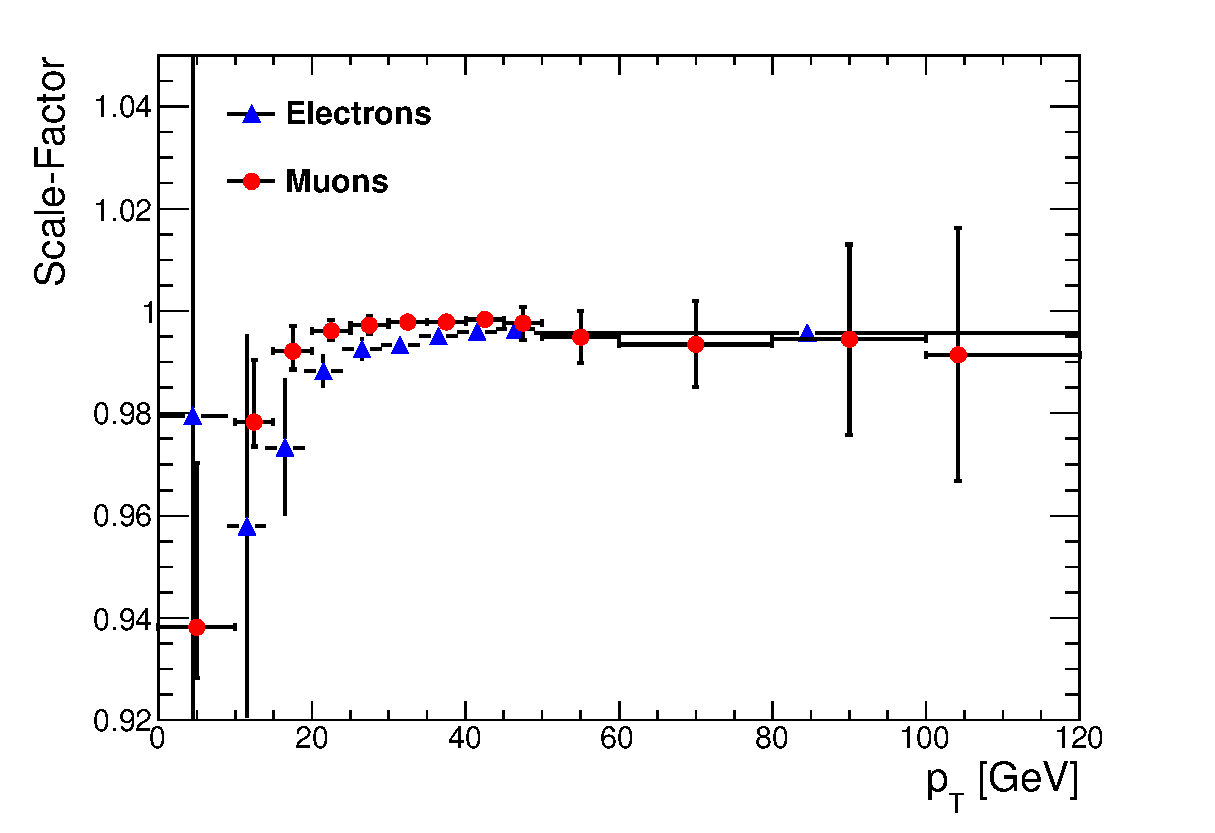
\includegraphics[width=0.7\textwidth]{MuonElectronIsoIPSF_130217}
        }
    \caption[Efficiency-correction scale-factors for the
  ${d_{0}}$ significance, $z_{0}\cdot sin(\theta)$ and track isolation cuts for
  electrons and muons in the 8~\tev\ data, as
  a function $p_{T}$ of the lepton.]{
Efficiency-correction scale-factors for the
  ${d_{0}}$ significance, $z_{0}\cdot sin(\theta)$ and track isolation cuts for
  electrons and muons in the 8~\tev\ data, as
  a function $p_{T}$ of the lepton.  The errors shown are a
  combination of the statistical and systematical uncertainties.
    }
\label{fig:iso-ip-sf-eight} 
\end{figure}

\subsubsection{Muon Systematic Uncertainties}

\begin{itemize}
     \item {\bf Reconstruction Efficiency:}
     Similarly to the electrons, uncertainties arise from the measurement of the
     muon reconstruction efficiency in data.

    \item {\bf Energy Scale:} For the 7~\tev\ analysis, uncertainties on the muon energy scale are
    conservatively estimated by taking the difference between the values of \CZZ\
    obtained with and without the energy scale correction applied. For the
    8~\tev\ analysis, the systematic is estimated by varying the energy scale
    correction applied to the \mc\ up and down by the 1-sigma uncertainty on the
    correction.

    \item {\bf Energy Resolution:} The energy resolution is measured separately
    for the muon inner detector and muon spectrometer track. Uncertainties are
    estimated by varying the amount of smearing applied to the muon ID and MS
    measurements separately. 
    
    \item {\bf Isolation/\zzero/\dzero\ Efficiency:} Similarly to the electron case,
    the efficiency of the additional muon selection cuts (isolation, \zzero,
    \dzerosig) is estimated from data using a tag and probe technique on \Zmm\
    decays. As for electrons, the 7~\tev\ data and \mc\ are found to be in 
    agreement with the uncertainty of the scale-factor measurement, so no correction is made to the central value of the \mc\ and
    uncertainties on the efficiency are propagated to the uncertainty on \CZZ. For the 8~\tev\
    analysis, scale-factors are applied to correct the efficiency of the \mc\, and the uncertainty on the
    scale-factor is taken as a systematic. The scale-factors applied at 8~\tev,
    and their uncertainty, are shown in~\fig{iso-ip-sf-eight}.

\end{itemize}

\subsubsection{Trigger Systematic Uncertainty}

Uncertainties arise on the measurement of the single-lepton efficiency in data.
These are propagated to \CZZ\ by varying the single-lepton trigger efficiencies
in~\eqn{triggerEffSF} up and down by their 1-sigma uncertainties.

\subsubsection{Theoretical Systematic Uncertainty}

Theoretical uncertainties to the \CZZ\ estimation arise due to the choice of
factorisation and renormalisation scale, the choice of PDF set, and from differences
arising due to different kinematic distributions obtained from different from \mc\
generators, due to, for example, different parton shower models and different
models for QED radiation.

The systematic due to the \mc\ generator is evaluated by comparing three \qqZZ\ \mc\ samples, generated
using different generators, PDF sets and scales. A
comparison is made between the default \powhegbox\ generated using the CT10 PDF
set and scale \mZZ, \pythia, generated using the MRST modified LO PDF set and scale
set to the arithmetic mean of the squared transverse masses of the two outgoing
particles ($(m^{2}_{T}(Z1)+m^{2}_{T}(Z2)/2$), and
\sherpa, generated using CTEQ6L1 PDF set and scale set to
($(m^{2}_{}(Z1)+p^{2}_{T}(Z1)+m^{2}_{}(Z2)p^{2}_{T}(Z2)/2$), and with a different
model for QED radiation as described in~\sec{gen-comparisons}.
Table~\ref{table:objSel-syst-genComp-seven} compares the \CZZ\ for the \qqZZ\
process obtained from \powhegbox, \sherpa\ and \pythia, as well as the for the
\ggZZ\ process obtained from \ggtwoZZ. Also shown is the combination of
the \CZZ\ from \powhegbox\ and \ggtwoZZ, weighted by the relative contributions
of the $qq$ and $gg$ processes to the fiducial \cx; this final number is the one
used in the \cx\ calculation. The largest difference between \powhegbox\ and
either \pythia\ or \sherpa\ is taken as the systematic uncertainty.

The effect of the scale and PDF set are assessed by
reweighting the \powhegbox\ sample to a scale of $\frac{1}{4}$\mZZ\ and to a
scale of \mZZ from its default scale of $\frac{1}{2}$\mZZ, and by reweighting
to the MSTW08 PDF set. This is done for the 8~\tev\ analysis; the resulting
variations on \CZZ\ are small, and are much smaller than the systematic from comparing
different generators, so for the 7~\tev\ analysis the systematic from generator
comparisons is taken to cover differences arising from PDF set and scale choice.

\begin{table}[htbp]
    \centering
    \small
    \begin{tabular}{l c c c c}

        \hline\hline

        \ZZ, 7~\tev & \eeee & \mmmm & \eemm & \llll \\

        \hline
        \multicolumn{5}{l}{\bf $qq$ Processes} \\

        PowhegBox   & \ZZSevenTeVCzzZZPowhegBoxEEEE\ $\pm$ \ZZSevenTeVCzzZZStatPowhegBoxEEEE 
                    & \ZZSevenTeVCzzZZPowhegBoxMMMM\ $\pm$ \ZZSevenTeVCzzZZStatPowhegBoxMMMM
                    & \ZZSevenTeVCzzZZPowhegBoxEEMM\ $\pm$ \ZZSevenTeVCzzZZStatPowhegBoxEEMM 
                    & \ZZSevenTeVCzzZZPowhegBoxLLLL\ $\pm$ \ZZSevenTeVCzzZZStatPowhegBoxLLLL \\

        \sherpa\    & \ZZSevenTeVCzzZZSherpaEEEE\ $\pm$ \ZZSevenTeVCzzZZStatSherpaEEEE 
                    & \ZZSevenTeVCzzZZSherpaMMMM\ $\pm$ \ZZSevenTeVCzzZZStatSherpaMMMM
                    & \ZZSevenTeVCzzZZSherpaEEMM\ $\pm$ \ZZSevenTeVCzzZZStatSherpaEEMM 
                    & \ZZSevenTeVCzzZZSherpaLLLL\ $\pm$ \ZZSevenTeVCzzZZStatSherpaLLLL \\

        \pythia     & \ZZSevenTeVCzzZZPythiaEEEE\ $\pm$ \ZZSevenTeVCzzZZStatPythiaEEEE 
                    & \ZZSevenTeVCzzZZPythiaMMMM\ $\pm$ \ZZSevenTeVCzzZZStatPythiaMMMM
                    & \ZZSevenTeVCzzZZPythiaEEMM\ $\pm$ \ZZSevenTeVCzzZZStatPythiaEEMM 
                    & \ZZSevenTeVCzzZZPythiaLLLL\ $\pm$ \ZZSevenTeVCzzZZStatPythiaLLLL \\

        \hline
        \multicolumn{5}{l}{\bf $gg$ Processes} \\
        \ggtwoZZ    & \ZZSevenTeVCzzZZggtwoZZEEEE\ $\pm$ \ZZSevenTeVCzzZZStatggtwoZZEEEE 
                    & \ZZSevenTeVCzzZZggtwoZZMMMM\ $\pm$ \ZZSevenTeVCzzZZStatggtwoZZMMMM
                    & \ZZSevenTeVCzzZZggtwoZZEEMM\ $\pm$ \ZZSevenTeVCzzZZStatggtwoZZEEMM 
                    & \ZZSevenTeVCzzZZggtwoZZLLLL\ $\pm$ \ZZSevenTeVCzzZZStatggtwoZZLLLL \\

        \hline
        \multicolumn{5}{l}{\bf Combined} \\
        PowhegBox+\ggtwoZZ\   
                    & \ZZSevenTeVCzzZZEEEE\ $\pm$ \ZZSevenTeVCzzZZStatEEEE 
                    & \ZZSevenTeVCzzZZMMMM\ $\pm$ \ZZSevenTeVCzzZZStatMMMM
                    & \ZZSevenTeVCzzZZEEMM\ $\pm$ \ZZSevenTeVCzzZZStatEEMM 
                    & \ZZSevenTeVCzzZZLLLL\ $\pm$ \ZZSevenTeVCzzZZStatLLLL \\

        \hline\hline
        \\
        \hline\hline

        \ZZs, 7~\tev & \eeee & \mmmm & \eemm & \llll \\

        \hline
        \multicolumn{5}{l}{\bf $qq$ Processes} \\

        PowhegBox   & \ZZSevenTeVCzzZZsPowhegBoxEEEE\ $\pm$ \ZZSevenTeVCzzZZsStatPowhegBoxEEEE 
                    & \ZZSevenTeVCzzZZsPowhegBoxMMMM\ $\pm$ \ZZSevenTeVCzzZZsStatPowhegBoxMMMM
                    & \ZZSevenTeVCzzZZsPowhegBoxEEMM\ $\pm$ \ZZSevenTeVCzzZZsStatPowhegBoxEEMM 
                    & \ZZSevenTeVCzzZZsPowhegBoxLLLL\ $\pm$ \ZZSevenTeVCzzZZsStatPowhegBoxLLLL \\

        \sherpa\    & \ZZSevenTeVCzzZZsSherpaEEEE\ $\pm$ \ZZSevenTeVCzzZZsStatSherpaEEEE 
                    & \ZZSevenTeVCzzZZsSherpaMMMM\ $\pm$ \ZZSevenTeVCzzZZsStatSherpaMMMM
                    & \ZZSevenTeVCzzZZsSherpaEEMM\ $\pm$ \ZZSevenTeVCzzZZsStatSherpaEEMM 
                    & \ZZSevenTeVCzzZZsSherpaLLLL\ $\pm$ \ZZSevenTeVCzzZZsStatSherpaLLLL \\

        \pythia     & \ZZSevenTeVCzzZZsPythiaEEEE\ $\pm$ \ZZSevenTeVCzzZZsStatPythiaEEEE 
                    & \ZZSevenTeVCzzZZsPythiaMMMM\ $\pm$ \ZZSevenTeVCzzZZsStatPythiaMMMM
                    & \ZZSevenTeVCzzZZsPythiaEEMM\ $\pm$ \ZZSevenTeVCzzZZsStatPythiaEEMM 
                    & \ZZSevenTeVCzzZZsPythiaLLLL\ $\pm$ \ZZSevenTeVCzzZZsStatPythiaLLLL \\

        \hline
        \multicolumn{5}{l}{\bf $gg$ Processes} \\
        \ggtwoZZ    & \ZZSevenTeVCzzZZsggtwoZZEEEE\ $\pm$ \ZZSevenTeVCzzZZsStatggtwoZZEEEE 
                    & \ZZSevenTeVCzzZZsggtwoZZMMMM\ $\pm$ \ZZSevenTeVCzzZZsStatggtwoZZMMMM
                    & \ZZSevenTeVCzzZZsggtwoZZEEMM\ $\pm$ \ZZSevenTeVCzzZZsStatggtwoZZEEMM 
                    & \ZZSevenTeVCzzZZsggtwoZZLLLL\ $\pm$ \ZZSevenTeVCzzZZsStatggtwoZZLLLL \\

        \hline
        \multicolumn{5}{l}{\bf Combined} \\
        PowhegBox+\ggtwoZZ\   
                    & \ZZSevenTeVCzzZZsEEEE\ $\pm$ \ZZSevenTeVCzzZZsStatEEEE 
                    & \ZZSevenTeVCzzZZsMMMM\ $\pm$ \ZZSevenTeVCzzZZsStatMMMM
                    & \ZZSevenTeVCzzZZsEEMM\ $\pm$ \ZZSevenTeVCzzZZsStatEEMM 
                    & \ZZSevenTeVCzzZZsLLLL\ $\pm$ \ZZSevenTeVCzzZZsStatLLLL \\

        \hline\hline
    \end{tabular}
    \caption[Reconstruction Acceptance \CZZ, compared between different MC
    generators for the 7~\tev\ analysis.]{
    Reconstruction Acceptance \CZZ, compared between different MC
    generators for the 7~\tev\ analysis. The \CZZ\ used in the \cx\ extraction is the
    weighted average of the \CZZ\ from \powhegbox\ and \ggtwoZZ\ generators, weighting
    by the relative contribution to the fiducial cross-section, as show in~\tab{theory-gg-frac}.
    The difference between \powhegbox\ and \sherpa\ is taken as an additional
    systematic uncertainty.
    Only the statistical uncertainty is shown. 
    }
    \label{table:objSel-syst-genComp-seven}
\end{table}

\begin{table}[htbp]
    \centering
    \small
    \begin{tabular}{l c c c c}

        \hline\hline

        \ZZ, 8~\tev & \eeee & \mmmm & \eemm & \llll \\

        \hline
        \multicolumn{5}{l}{\bf $qq$ Processes} \\

        PowhegBox   & \ZZEightTeVCzzZZPowhegBoxEEEE\ $\pm$ \ZZEightTeVCzzZZStatPowhegBoxEEEE 
                    & \ZZEightTeVCzzZZPowhegBoxMMMM\ $\pm$ \ZZEightTeVCzzZZStatPowhegBoxMMMM
                    & \ZZEightTeVCzzZZPowhegBoxEEMM\ $\pm$ \ZZEightTeVCzzZZStatPowhegBoxEEMM 
                    & \ZZEightTeVCzzZZPowhegBoxLLLL\ $\pm$ \ZZEightTeVCzzZZStatPowhegBoxLLLL \\

        \sherpa\    & \ZZEightTeVCzzZZSherpaEEEE\ $\pm$ \ZZEightTeVCzzZZStatSherpaEEEE 
                    & \ZZEightTeVCzzZZSherpaMMMM\ $\pm$ \ZZEightTeVCzzZZStatSherpaMMMM
                    & \ZZEightTeVCzzZZSherpaEEMM\ $\pm$ \ZZEightTeVCzzZZStatSherpaEEMM 
                    & \ZZEightTeVCzzZZSherpaLLLL\ $\pm$ \ZZEightTeVCzzZZStatSherpaLLLL \\

        \pythia     & \ZZEightTeVCzzZZPythiaEEEE\ $\pm$ \ZZEightTeVCzzZZStatPythiaEEEE 
                    & \ZZEightTeVCzzZZPythiaMMMM\ $\pm$ \ZZEightTeVCzzZZStatPythiaMMMM
                    & \ZZEightTeVCzzZZPythiaEEMM\ $\pm$ \ZZEightTeVCzzZZStatPythiaEEMM 
                    & \ZZEightTeVCzzZZPythiaLLLL\ $\pm$ \ZZEightTeVCzzZZStatPythiaLLLL \\

        \hline
        \multicolumn{5}{l}{\bf $gg$ Processes} \\
        \ggtwoZZ    & \ZZEightTeVCzzZZggtwoZZEEEE\ $\pm$ \ZZEightTeVCzzZZStatggtwoZZEEEE 
                    & \ZZEightTeVCzzZZggtwoZZMMMM\ $\pm$ \ZZEightTeVCzzZZStatggtwoZZMMMM
                    & \ZZEightTeVCzzZZggtwoZZEEMM\ $\pm$ \ZZEightTeVCzzZZStatggtwoZZEEMM 
                    & \ZZEightTeVCzzZZggtwoZZLLLL\ $\pm$ \ZZEightTeVCzzZZStatggtwoZZLLLL \\

        \hline
        \multicolumn{5}{l}{\bf Combined} \\
        PowhegBox+\ggtwoZZ\   
                    & \ZZEightTeVCzzZZEEEE\ $\pm$ \ZZEightTeVCzzZZStatEEEE 
                    & \ZZEightTeVCzzZZMMMM\ $\pm$ \ZZEightTeVCzzZZStatMMMM
                    & \ZZEightTeVCzzZZEEMM\ $\pm$ \ZZEightTeVCzzZZStatEEMM 
                    & \ZZEightTeVCzzZZLLLL\ $\pm$ \ZZEightTeVCzzZZStatLLLL \\

        \hline\hline
        %\\
        %\hline\hline

        %\ZZs, 8~\tev & \eeee & \mmmm & \eemm & \llll \\

        %\hline
        %\multicolumn{5}{l}{\bf $qq$ Processes} \\

        %PowhegBox   & \ZZEightTeVCzzZZsPowhegBoxEEEE\ $\pm$ \ZZEightTeVCzzZZsStatPowhegBoxEEEE 
        %            & \ZZEightTeVCzzZZsPowhegBoxMMMM\ $\pm$ \ZZEightTeVCzzZZsStatPowhegBoxMMMM
        %            & \ZZEightTeVCzzZZsPowhegBoxEEMM\ $\pm$ \ZZEightTeVCzzZZsStatPowhegBoxEEMM 
        %            & \ZZEightTeVCzzZZsPowhegBoxLLLL\ $\pm$ \ZZEightTeVCzzZZsStatPowhegBoxLLLL \\

        %\sherpa\    & \ZZEightTeVCzzZZsStatSherpaEEEE\ $\pm$ \ZZEightTeVCzzZZsStatSherpaEEEE 
        %            & \ZZEightTeVCzzZZsStatSherpaMMMM\ $\pm$ \ZZEightTeVCzzZZsStatSherpaMMMM
        %            & \ZZEightTeVCzzZZsStatSherpaEEMM\ $\pm$ \ZZEightTeVCzzZZsStatSherpaEEMM 
        %            & \ZZEightTeVCzzZZsStatSherpaLLLL\ $\pm$ \ZZEightTeVCzzZZsStatSherpaLLLL \\

        %\pythia     & \ZZEightTeVCzzZZsPythiaEEEE\ $\pm$ \ZZEightTeVCzzZZsStatPythiaEEEE 
        %            & \ZZEightTeVCzzZZsPythiaMMMM\ $\pm$ \ZZEightTeVCzzZZsStatPythiaMMMM
        %            & \ZZEightTeVCzzZZsPythiaEEMM\ $\pm$ \ZZEightTeVCzzZZsStatPythiaEEMM 
        %            & \ZZEightTeVCzzZZsPythiaLLLL\ $\pm$ \ZZEightTeVCzzZZsStatPythiaLLLL \\

        %\hline
        %\multicolumn{5}{l}{\bf $gg$ Processes} \\
        %\ggtwoZZ    & \ZZEightTeVCzzZZsggtwoZZEEEE\ $\pm$ \ZZEightTeVCzzZZsStatggtwoZZEEEE 
        %            & \ZZEightTeVCzzZZsggtwoZZMMMM\ $\pm$ \ZZEightTeVCzzZZsStatggtwoZZMMMM
        %            & \ZZEightTeVCzzZZsggtwoZZEEMM\ $\pm$ \ZZEightTeVCzzZZsStatggtwoZZEEMM 
        %            & \ZZEightTeVCzzZZsggtwoZZLLLL\ $\pm$ \ZZEightTeVCzzZZsStatggtwoZZLLLL \\

        %\hline
        %\multicolumn{5}{l}{\bf Combined} \\
        %PowhegBox+\ggtwoZZ\   
        %            & \ZZEightTeVCzzZZsEEEE\ $\pm$ \ZZEightTeVCzzZZsStatEEEE 
        %            & \ZZEightTeVCzzZZsMMMM\ $\pm$ \ZZEightTeVCzzZZsStatMMMM
        %            & \ZZEightTeVCzzZZsEEMM\ $\pm$ \ZZEightTeVCzzZZsStatEEMM 
        %            & \ZZEightTeVCzzZZsLLLL\ $\pm$ \ZZEightTeVCzzZZsStatLLLL \\

        %\hline\hline
    \end{tabular}
    \caption[Reconstruction Acceptance \CZZ, compared between different MC
    generators for the 8~\tev\ analysis.]{Reconstruction Acceptance \CZZ, compared between different MC
    generators for the 8~\tev\ analysis. The \CZZ\ used in the \cx\ extraction is the
    weighted average of the \CZZ\ from \powhegbox\ and \ggtwoZZ\ generators, weighting
    by the relative contribution to the fiducial cross-section, as show in~\tab{theory-gg-frac}.
    The difference between \powhegbox\ and \sherpa\ is taken as an additional
    systematic uncertainty.
    Only the statistical uncertainty is shown. 
    }
    \label{table:objSel-syst-genComp-eight}
\end{table}

\subsection{Systematic Uncertainty Estimates}

The effect of each of the systematic uncertainties described above on \CZZ\ is estimated using
the \powhegbox\ and \ggZZ\ \mc. The resulting shifts in the value of \CZZ\ in
percent are shown in~\tab{objSel-syst-seven} for the 7~\tev\ analysis and
in~\tab{objSel-syst-eight} for the 8~\tev\ analysis, as well as the total
uncertainty obtained by summing each source in quadrature. The
dominant sources of systematic uncertainty are the electron and muon reconstruction,
identification and isolation/z0/d0Sig efficiencies. The
uncertainty in the \eeee\ final state is over twice as large as for the \mmmm\
final state, due to the larger reconstruction and identification uncertainties
for electrons.

\begin{table}[htbp]
   \centering
   \small
   \begin{tabular}{l c c c c}
      \hline\hline
      \ZZ\ Selection, 7~\tev\               & \eeee           & \mmmm                  & \eemm                    & \llll                      \\
      \hline
      \multicolumn{4}{l}{\bf Reconstruction Uncertainties (\%)} \\
      $e$ energy scale                      & \ZZSevenTeVSystematicZZEScaleEEEE           & \ZZSevenTeVSystematicZZEScaleMMMM    
                                            & \ZZSevenTeVSystematicZZEScaleEEMM           & \ZZSevenTeVSystematicZZEScaleLLLL    \\
      $e$ energy resolution                 & \ZZSevenTeVSystematicZZESmearEEEE           & \ZZSevenTeVSystematicZZESmearMMMM    
                                            & \ZZSevenTeVSystematicZZESmearEEMM           & \ZZSevenTeVSystematicZZESmearLLLL    \\
      $e$ reconstruction efficiency         & \ZZSevenTeVSystematicZZERecoEEEE            & \ZZSevenTeVSystematicZZERecoMMMM     
                                            & \ZZSevenTeVSystematicZZERecoEEMM            & \ZZSevenTeVSystematicZZERecoLLLL     \\
      $e$ identification efficiency         & \ZZSevenTeVSystematicZZEIdEEEE              & \ZZSevenTeVSystematicZZEIdMMMM       
                                            & \ZZSevenTeVSystematicZZEIdEEMM              & \ZZSevenTeVSystematicZZEIdLLLL       \\
      $e$ isolation/z0/d0Sig efficiency     & \ZZSevenTeVSystematicZZEIsoEEEE             & \ZZSevenTeVSystematicZZEIsoMMMM      
                                            & \ZZSevenTeVSystematicZZEIsoEEMM             & \ZZSevenTeVSystematicZZEIsoLLLL      \\
      $\mu$ momentum scale                  & \ZZSevenTeVSystematicZZMuScaleEEEE          & \ZZSevenTeVSystematicZZMuScaleMMMM   
                                            & \ZZSevenTeVSystematicZZMuScaleEEMM          & \ZZSevenTeVSystematicZZMuScaleLLLL   \\
      $\mu$ momentum resolution             & \ZZSevenTeVSystematicZZMuSmearEEEE          & \ZZSevenTeVSystematicZZMuSmearMMMM   
                                            & \ZZSevenTeVSystematicZZMuSmearEEMM          & \ZZSevenTeVSystematicZZMuSmearLLLL \\
      $\mu$ reconstruction efficiency       & \ZZSevenTeVSystematicZZMuRecoEEEE           & \ZZSevenTeVSystematicZZMuRecoMMMM    
                                            & \ZZSevenTeVSystematicZZMuRecoEEMM           & \ZZSevenTeVSystematicZZMuRecoLLLL    \\
      $\mu$ isolation/z0/d0Sig efficiency   & \ZZSevenTeVSystematicZZMuIsoEEEE            & \ZZSevenTeVSystematicZZMuIsoMMMM     
                                            & \ZZSevenTeVSystematicZZMuIsoEEMM            & \ZZSevenTeVSystematicZZMuIsoLLLL     \\
      IP Resolution                         & \ZZSevenTeVSystematicZZIPResEEEE            & \ZZSevenTeVSystematicZZIPResMMMM  
                                            & \ZZSevenTeVSystematicZZIPResEEMM            & \ZZSevenTeVSystematicZZIPResLLLL  \\
      Trigger                               & \ZZSevenTeVSystematicZZOverallTriggerEEEE   & \ZZSevenTeVSystematicZZOverallTriggerMMMM  
                                            & \ZZSevenTeVSystematicZZOverallTriggerEEMM   & \ZZSevenTeVSystematicZZOverallTriggerLLLL  \\
      \hline
      Total Reconstruction                  & \ZZSevenTeVSystematicZZRecoTotalEEEE        & \ZZSevenTeVSystematicZZRecoTotalMMMM 
                                            & \ZZSevenTeVSystematicZZRecoTotalEEMM        & \ZZSevenTeVSystematicZZRecoTotalLLLL \\
      \hline
      \multicolumn{4}{l}{\bf Theoretical Uncertainties (\%)} \\
      MC Generator Difference               & \ZZSevenTeVSystematicZZGeneratorEEEE        & \ZZSevenTeVSystematicZZGeneratorMMMM 
                                            & \ZZSevenTeVSystematicZZGeneratorEEMM        & \ZZSevenTeVSystematicZZGeneratorLLLL \\
      \hline
      {\bf Total \CZZ\ Uncertainty}         & \ZZSevenTeVSystematicZZCzzTotalEEEE         & \ZZSevenTeVSystematicZZCzzTotalMMMM 
                                            & \ZZSevenTeVSystematicZZCzzTotalEEMM         & \ZZSevenTeVSystematicZZCzzTotalLLLL \\
      \hline\hline
      \\
      \hline\hline
      \ZZs\ Selection, 7~\tev\               & \eeee           & \mmmm                  & \eemm                    & \llll                      \\
      \hline
      \multicolumn{4}{l}{\bf Reconstruction Uncertainties (\%)} \\
      $e$ energy scale                      & \ZZSevenTeVSystematicZZsEScaleEEEE           & \ZZSevenTeVSystematicZZsEScaleMMMM    
                                            & \ZZSevenTeVSystematicZZsEScaleEEMM           & \ZZSevenTeVSystematicZZsEScaleLLLL    \\
      $e$ energy resolution                 & \ZZSevenTeVSystematicZZsESmearEEEE           & \ZZSevenTeVSystematicZZsESmearMMMM    
                                            & \ZZSevenTeVSystematicZZsESmearEEMM           & \ZZSevenTeVSystematicZZsESmearLLLL    \\
      $e$ reconstruction efficiency         & \ZZSevenTeVSystematicZZsERecoEEEE            & \ZZSevenTeVSystematicZZsERecoMMMM     
                                            & \ZZSevenTeVSystematicZZsERecoEEMM            & \ZZSevenTeVSystematicZZsERecoLLLL     \\
      $e$ identification efficiency         & \ZZSevenTeVSystematicZZsEIdEEEE              & \ZZSevenTeVSystematicZZsEIdMMMM       
                                            & \ZZSevenTeVSystematicZZsEIdEEMM              & \ZZSevenTeVSystematicZZsEIdLLLL       \\
      $e$ isolation/z0/d0Sig efficiency     & \ZZSevenTeVSystematicZZsEIsoEEEE             & \ZZSevenTeVSystematicZZsEIsoMMMM      
                                            & \ZZSevenTeVSystematicZZsEIsoEEMM             & \ZZSevenTeVSystematicZZsEIsoLLLL      \\
      $\mu$ momentum scale                  & \ZZSevenTeVSystematicZZsMuScaleEEEE          & \ZZSevenTeVSystematicZZsMuScaleMMMM   
                                            & \ZZSevenTeVSystematicZZsMuScaleEEMM          & \ZZSevenTeVSystematicZZsMuScaleLLLL   \\
      $\mu$ momentum resolution             & \ZZSevenTeVSystematicZZsMuSmearEEEE          & \ZZSevenTeVSystematicZZsMuSmearMMMM   
                                            & \ZZSevenTeVSystematicZZsMuSmearEEMM          & \ZZSevenTeVSystematicZZsMuSmearLLLL \\
      $\mu$ reconstruction efficiency       & \ZZSevenTeVSystematicZZsMuRecoEEEE           & \ZZSevenTeVSystematicZZsMuRecoMMMM    
                                            & \ZZSevenTeVSystematicZZsMuRecoEEMM           & \ZZSevenTeVSystematicZZsMuRecoLLLL    \\
      $\mu$ isolation/z0/d0Sig efficiency   & \ZZSevenTeVSystematicZZsMuIsoEEEE            & \ZZSevenTeVSystematicZZsMuIsoMMMM     
                                            & \ZZSevenTeVSystematicZZsMuIsoEEMM            & \ZZSevenTeVSystematicZZsMuIsoLLLL     \\
      IP Resolution                         & \ZZSevenTeVSystematicZZsIPResEEEE            & \ZZSevenTeVSystematicZZsIPResMMMM  
                                            & \ZZSevenTeVSystematicZZsIPResEEMM            & \ZZSevenTeVSystematicZZsIPResLLLL  \\
      Trigger                               & \ZZSevenTeVSystematicZZsOverallTriggerEEEE   & \ZZSevenTeVSystematicZZsOverallTriggerMMMM  
                                            & \ZZSevenTeVSystematicZZsOverallTriggerEEMM   & \ZZSevenTeVSystematicZZsOverallTriggerLLLL  \\
      \hline
      Total Reconstruction                  & \ZZSevenTeVSystematicZZsRecoTotalEEEE        & \ZZSevenTeVSystematicZZsRecoTotalMMMM 
                                            & \ZZSevenTeVSystematicZZsRecoTotalEEMM        & \ZZSevenTeVSystematicZZsRecoTotalLLLL \\
      \hline
      \multicolumn{4}{l}{\bf Theoretical Uncertainties (\%)} \\
      MC Generator Difference               & \ZZSevenTeVSystematicZZsGeneratorEEEE        & \ZZSevenTeVSystematicZZsGeneratorMMMM 
                                            & \ZZSevenTeVSystematicZZsGeneratorEEMM        & \ZZSevenTeVSystematicZZsGeneratorLLLL \\
      \hline
      {\bf Total \CZZ\ Uncertainty}         & \ZZSevenTeVSystematicZZsCzzTotalEEEE         & \ZZSevenTeVSystematicZZsCzzTotalMMMM 
                                            & \ZZSevenTeVSystematicZZsCzzTotalEEMM         & \ZZSevenTeVSystematicZZsCzzTotalLLLL \\
      \hline\hline

   \end{tabular}
   \caption[Systematic uncertainties to the reconstruction acceptance \CZZ\ for
   the 7~\tev\ analysis.]
   {Summary of systematic uncertainties to the reconstruction acceptance \CZZ\
   in percent, by \ZZ\ final state, for the 7~\tev\ analysis. The top table
   gives uncertainties to the \ZZ\ selection, the bottom to the \ZZs\ selection.
   The fourth column gives the weighted average
   of the three final states. The total uncertainty is also given, which is the
   sum in quadrature of the individual uncertainties.} 
   \label{table:objSel-syst-seven}
\end{table}

%%%%%%%%%%%%%%%%%%%%%%%%
% Systematics 8 TeV
\begin{table}[htbp]
   \centering
   \small
   \begin{tabular}{l c c c c}
      \hline\hline
      \ZZ\ Selection, 8~\tev\               & \eeee           & \mmmm                  & \eemm                    & \llll                      \\
      \hline
      \multicolumn{4}{l}{\bf Reconstruction Uncertainties (\%)} \\
      $e$ energy scale                      & \ZZEightTeVSystematicZZEScaleEEEE           & \ZZEightTeVSystematicZZEScaleMMMM    
                                            & \ZZEightTeVSystematicZZEScaleEEMM           & \ZZEightTeVSystematicZZEScaleLLLL    \\
      $e$ energy resolution                 & \ZZEightTeVSystematicZZESmearEEEE           & \ZZEightTeVSystematicZZESmearMMMM    
                                            & \ZZEightTeVSystematicZZESmearEEMM           & \ZZEightTeVSystematicZZESmearLLLL    \\
      $e$ reconstruction efficiency         & \ZZEightTeVSystematicZZERecoEEEE            & \ZZEightTeVSystematicZZERecoMMMM     
                                            & \ZZEightTeVSystematicZZERecoEEMM            & \ZZEightTeVSystematicZZERecoLLLL     \\
      $e$ identification efficiency         & \ZZEightTeVSystematicZZEIdEEEE              & \ZZEightTeVSystematicZZEIdMMMM       
                                            & \ZZEightTeVSystematicZZEIdEEMM              & \ZZEightTeVSystematicZZEIdLLLL       \\
      $e$ isolation/z0/d0Sig efficiency     & \ZZEightTeVSystematicZZEIsoEEEE             & \ZZEightTeVSystematicZZEIsoMMMM      
                                            & \ZZEightTeVSystematicZZEIsoEEMM             & \ZZEightTeVSystematicZZEIsoLLLL      \\
      $\mu$ momentum scale                  & \ZZEightTeVSystematicZZMuScaleEEEE          & \ZZEightTeVSystematicZZMuScaleMMMM   
                                            & \ZZEightTeVSystematicZZMuScaleEEMM          & \ZZEightTeVSystematicZZMuScaleLLLL   \\
      $\mu$ momentum resolution             & \ZZEightTeVSystematicZZMuSmearEEEE          & \ZZEightTeVSystematicZZMuSmearMMMM   
                                            & \ZZEightTeVSystematicZZMuSmearEEMM          & \ZZEightTeVSystematicZZMuSmearLLLL \\
      $\mu$ reconstruction efficiency       & \ZZEightTeVSystematicZZMuRecoEEEE           & \ZZEightTeVSystematicZZMuRecoMMMM    
                                            & \ZZEightTeVSystematicZZMuRecoEEMM           & \ZZEightTeVSystematicZZMuRecoLLLL    \\
      $\mu$ isolation/z0/d0Sig efficiency   & \ZZEightTeVSystematicZZMuIsoEEEE            & \ZZEightTeVSystematicZZMuIsoMMMM     
                                            & \ZZEightTeVSystematicZZMuIsoEEMM            & \ZZEightTeVSystematicZZMuIsoLLLL     \\
      Trigger                               & \ZZEightTeVSystematicZZOverallTriggerEEEE   & \ZZEightTeVSystematicZZOverallTriggerMMMM  
                                            & \ZZEightTeVSystematicZZOverallTriggerEEMM   & \ZZEightTeVSystematicZZOverallTriggerLLLL  \\
      \hline
      Total Reconstruction                  & \ZZEightTeVSystematicZZRecoTotalEEEE        & \ZZEightTeVSystematicZZRecoTotalMMMM 
                                            & \ZZEightTeVSystematicZZRecoTotalEEMM        & \ZZEightTeVSystematicZZRecoTotalLLLL \\
      \hline
      \multicolumn{4}{l}{\bf Theoretical Uncertainties (\%)} \\
      MC Generator Difference               & \ZZEightTeVSystematicZZGeneratorEEEE        & \ZZEightTeVSystematicZZGeneratorMMMM 
                                            & \ZZEightTeVSystematicZZGeneratorEEMM        & \ZZEightTeVSystematicZZGeneratorLLLL \\
      \hline
      {\bf Total \CZZ\ Uncertainty}         & \ZZEightTeVSystematicZZCzzTotalEEEE         & \ZZEightTeVSystematicZZCzzTotalMMMM 
                                            & \ZZEightTeVSystematicZZCzzTotalEEMM         & \ZZEightTeVSystematicZZCzzTotalLLLL \\
      \hline\hline
      %\\
      %\hline\hline
      %\ZZs\ Selection, 8~\tev\               & \eeee           & \mmmm                  & \eemm                    & \llll                      \\
      %\hline
      %\multicolumn{4}{l}{\bf Reconstruction Uncertainties (\%)} \\
      %$e$ energy scale                      & \ZZEightTeVSystematicZZsEScaleEEEE           & \ZZEightTeVSystematicZZsEScaleMMMM    
      %                                      & \ZZEightTeVSystematicZZsEScaleEEMM           & \ZZEightTeVSystematicZZsEScaleLLLL    \\
      %$e$ energy resolution                 & \ZZEightTeVSystematicZZsESmearEEEE           & \ZZEightTeVSystematicZZsESmearMMMM    
      %                                      & \ZZEightTeVSystematicZZsESmearEEMM           & \ZZEightTeVSystematicZZsESmearLLLL    \\
      %$e$ reconstruction efficiency         & \ZZEightTeVSystematicZZsERecoEEEE            & \ZZEightTeVSystematicZZsERecoMMMM     
      %                                      & \ZZEightTeVSystematicZZsERecoEEMM            & \ZZEightTeVSystematicZZsERecoLLLL     \\
      %$e$ identification efficiency         & \ZZEightTeVSystematicZZsEIdEEEE              & \ZZEightTeVSystematicZZsEIdMMMM       
      %                                      & \ZZEightTeVSystematicZZsEIdEEMM              & \ZZEightTeVSystematicZZsEIdLLLL       \\
      %$e$ isolation/z0/d0Sig efficiency     & \ZZEightTeVSystematicZZsEIsoEEEE             & \ZZEightTeVSystematicZZsEIsoMMMM      
      %                                      & \ZZEightTeVSystematicZZsEIsoEEMM             & \ZZEightTeVSystematicZZsEIsoLLLL      \\
      %$\mu$ momentum scale                  & \ZZEightTeVSystematicZZsMuScaleEEEE          & \ZZEightTeVSystematicZZsMuScaleMMMM   
      %                                      & \ZZEightTeVSystematicZZsMuScaleEEMM          & \ZZEightTeVSystematicZZsMuScaleLLLL   \\
      %$\mu$ momentum resolution             & \ZZEightTeVSystematicZZsMuSmearEEEE          & \ZZEightTeVSystematicZZsMuSmearMMMM   
      %                                      & \ZZEightTeVSystematicZZsMuSmearEEMM          & \ZZEightTeVSystematicZZsMuSmearLLLL \\
      %$\mu$ reconstruction efficiency       & \ZZEightTeVSystematicZZsMuRecoEEEE           & \ZZEightTeVSystematicZZsMuRecoMMMM    
      %                                      & \ZZEightTeVSystematicZZsMuRecoEEMM           & \ZZEightTeVSystematicZZsMuRecoLLLL    \\
      %$\mu$ isolation/z0/d0Sig efficiency   & \ZZEightTeVSystematicZZsMuIsoEEEE            & \ZZEightTeVSystematicZZsMuIsoMMMM     
      %                                      & \ZZEightTeVSystematicZZsMuIsoEEMM            & \ZZEightTeVSystematicZZsMuIsoLLLL     \\
      %Trigger                               & \ZZEightTeVSystematicZZsOverallTriggerEEEE   & \ZZEightTeVSystematicZZsOverallTriggerMMMM  
      %                                      & \ZZEightTeVSystematicZZsOverallTriggerEEMM   & \ZZEightTeVSystematicZZsOverallTriggerLLLL  \\
      %\hline
      %Total Reconstruction                  & \ZZEightTeVSystematicZZsRecoTotalEEEE        & \ZZEightTeVSystematicZZsRecoTotalMMMM 
      %                                      & \ZZEightTeVSystematicZZsRecoTotalEEMM        & \ZZEightTeVSystematicZZsRecoTotalLLLL \\
      %\hline
      %\multicolumn{4}{l}{\bf Theoretical Uncertainties (\%)} \\
      %MC Generator Difference               & \ZZEightTeVSystematicZZsGeneratorEEEE        & \ZZEightTeVSystematicZZsGeneratorMMMM 
      %                                      & \ZZEightTeVSystematicZZsGeneratorEEMM        & \ZZEightTeVSystematicZZsGeneratorLLLL \\
      %\hline
      %{\bf Total \CZZ\ Uncertainty}         & \ZZEightTeVSystematicZZsCzzTotalEEEE         & \ZZEightTeVSystematicZZsCzzTotalMMMM 
      %                                      & \ZZEightTeVSystematicZZsCzzTotalEEMM         & \ZZEightTeVSystematicZZsCzzTotalLLLL \\
      %\hline\hline

   \end{tabular}
   \caption[Systematic uncertainties to the reconstruction acceptance \CZZ\ for
   the 8~\tev\ analysis.]
   {Summary of systematic uncertainties to the reconstruction acceptance \CZZ\
   in percent, by \ZZ\ final state, for the 8~\tev\ analysis. 
   %The top table
   %gives uncertainties to the \ZZ\ selection, the bottom to the \ZZs\ selection.
   The fourth column gives the weighted average
   of the three final states. The total uncertainty is also given, which is the
   sum in quadrature of the individual uncertainties.} 
   \label{table:objSel-syst-eight}
\end{table}
